\chapter{Probing assumptions in spherical deconvolution techniques}
\label{chap:frf_experiment}

\chaptertoc{}

\begin{chapterabstract}
This chapter presents a series of experiments performed using \acs{ConFiG} phantoms and real fibres reconstructed from \ac{EM} to probe assumptions inherent in \ac{dMRI} techniques based on \ac{SD} for estimating the \ac{FOD}.

Firstly, the theory behind \ac{SD} techniques is described, outlining the assumptions that are tested in this work. \ac{dMRI} simulations are performed in \acs{ConFiG} phantoms and \ac{EM} fibres to test how realistic, complex axonal morphology impacts \ac{SD} techniques for \ac{FOD} estimation. 
\end{chapterabstract}


\section{Introduction}
\label{sec:frf_introduction}
Diffusion weighted magnetic resonance imaging (dMRI) has been widely used to probe the structure and organisation of brain tissue, with one particular area of focus being the estimation of the orientational distribution of neuronal fibres in a voxel. This \ac{FOD} is particularly interesting since it is used in tractography techniques to probe the structural connectivity of the brain which is important in many clinical and basic neuroscience studies\cite{DellAcqua2019,Johansen-Berg2006,Catani2013}.
Whilst tractography has found many uses, there remain a number of challenges to the technique \cite{Jbabdi2011,Schilling2019b}, including typically generating a large number of false positive connections \cite{Maier-Hein2017}.
One potential source of these issues could be due to difficulties in reliably estimating the \ac{FOD}, where minor differences in \ac{FOD} could lead to large differences in the tractrograms created \cite{Schilling2019b}.
Accurate and reliable estimation of the \ac{FOD} is therefore important to improve the accuracy of tractography techniques.


Many techniques have been developed for estimating the \acl{FOD}, of which perhaps the most prominent are based on \acf{SD}. While there are a variety of spherical deconvolution methods, the central principle is the same - the diffusion weighted signal as a function of the azimuthal ($\phi$) and elevation ($\theta$) angles is modelled as a spherical convolution of the \ac{FOD}, $F(\theta,\phi)$, with a kernel (called the \ac{FRF}), $R(\theta)$, the typical diffusion weighted signal from a single fibre population estimated \emph{a priori}:
\begin{equation}
  S(\theta, \phi) = F(\theta, \phi) \otimes R(\theta) \,.
  \label{eq:spherical_conv}
\end{equation}

By modelling the signal in this way, a number of assumptions are made. For instance, the \ac{FRF} is typically estimated from a \ac{WM} region expected to contain a single bundle of coherent fibres and that \ac{FRF} is assumed to be constant throughout the rest of the \ac{WM}.
Recently, some works have challenged this assumption \cite{Novikov2019,Schilling2019,Christiaens2020}, for instance Schilling et al. \cite{Schilling2019} use known \acs{FOD}s from histology to estimate the \ac{FRF} in different WM regions, showing that the \ac{FRF} does indeed vary across the \ac{WM} and that this variation does affect the estimated \ac{FOD} and tractography results.

However, the assumption behind the \ac{FRF} not only requires it to be the same across WM voxels, but also to be identical across individual fibres within a voxel.
% No works, however, have looked to take this one step further, probing the assumption inherent in the \ac{FRF} definition that the response from each individual fibre in a voxel is the same.
Indeed, recent works using \ac{EM} to investigate \ac{WM} axonal morphology show that axons within a voxel have different shapes \cite{Lee2019b,Abdollahzadeh2019}. Axons have varying diameters along their length and are generally not straight, at least in part as a result of having to pack together around one another and other cells, so it is reasonable to expect that fibres will have different responses, contrary to this assumption.

A related factor is that this representation cannot properly account for non-straight fibres since an assumption is made that there is no exchange between fibres or, equivalently, between diffusion in different directions. In essence, this means that the fibres are implicitly assumed to be perfectly straight and pointing a given direction since any deviation from straight (i.e. curved or undulating fibres) would add directions that are dependent on one another.

% One further consideration is that the contribution of the extra-axonal space to the signal is not explicitly modelled. This means that either the extra-axonal signal should be assumed to be identical to the intra-axonal signal (meaning that it can be included in the \ac{FRF}) or that the extra-axonal space has a negligible contribution to the total signal.
One further consideration is that the contribution of the extra-axonal space to the signal is not explicitly modelled. The convolution in \Cref{eq:spherical_conv} assumes that there is no exchange between diffusion in different directions, meaning that should the extracellular space be included in the \ac{FRF}, then we must assume that the extracellular space does not exchange (which is unlikely due to its relatively unrestricted structure) or that its contribution is minimal.
Indeed, certain techniques using \ac{SD}, such \ac{AFD} \cite{Raffelt2012}, make this assumption explicitly, assuming that the extracellular signal is negligible at a high b-value (> 3000 \si{\second\per\milli\metre\squared}), though this has only been tested in simple numerical phantoms of straight parallel cylinders.
It may be the case that the realistic extra-axonal in complex fibre arrangements (such as with orientation dispersion or interleaved crossing bundles) behaves differently to this simple cylinder case, and may violate this assumption. 

\begin{comment}
Another assumption is that the \ac{FRF} is assumed to be the same for all fibres (or fibre populations) in the voxel, meaning that the overall signal is just this \ac{FRF} summed up across the orientations of all the fibres.
Additionally, this representation cannot properly account for non-straight fibres since an assumption is made that there is no exchange between fibres or, equivalently, between diffusion in different directions. In essence, this means that the fibres are implicitly assumed to be perfectly straight and pointing a given direction since any deviation from straight (i.e. curved or undulating fibres) would add directions that are dependent on one another.

In practice, however, it is not possible to have a large number of straight fibres pointing in different directions within the same space and maintain a high fibre volume fraction other than in a few simple cases such as planar dispersed cylinders. Ex vivo studies using 3D electron microscopy of mouse corpus callosum have shown than axons are generally not straight, at least in part as a result of having to pack together around one another and other cells.
\end{comment}

In this work we use \ac{ConFiG}, our recently developed white matter numerical phantom generator capable of generating realistic WM morphology, to investigate what effect, if any, violation of these assumptions introduced by realistic axonal morphologies has on have on the estimated \ac{FOD}.% these whether these assumptions hold in realistic axonal geometries.
Firstly, we investigate how the realistic packing of fibres affects the diffusion within each fibre and whether the dMRI signal from each fibre is the same, as \ac{SD} assumes.
As well as using \ac{ConFiG} phantoms, we use axons reconstructed from the \ac{EM} data from Lee at al. \cite{Lee2019b} to test the \ac{dMRI} signal in real axonal geometry.
Additionally, we investigate the contribution of the extracellular space to the total \ac{dMRI} signal, whether the extracellular signal is similar to intracellular signal and how much it contributes to the overall signal.

The rest of this chapter is organised as follows: \Cref{sec:frf_method} describes the experiments performed to probe the assumptions outlined above, \Cref{sec:frf_results} presents the results and \Cref{sec:frf_discussion,sec:frf_conclusion} summarise the contributions and discuss future work.


\section{Method}
\label{sec:frf_method}
% In order to test what impact the complex morphology introduced by packing fibres together has on the individual fibre response functions and how this varies from the straight fibre model used in SD a simulation experiment was performed in a set of numerical phantoms generated using ConFiG.
In order to test the assumptions in \ac{SD} techniques, experiments were performed in a range of numerical phantoms generated using ConFiG, using an acquisition typical of \ac{SD} applications. In this section, we describe the phantoms that we generate and the \ac{dMRI} simulation experiments that were performed to probe these assumptions.

\subsection{Phantom Generation}
\label{sec:frf_phantom_generation}
In order to test \ac{SD} techniques in realistic geometries, two sets of \ac{ConFiG} phantoms were generated for this work, one set of phantoms containing a single bundle of fibres with varying amounts of orientation dispersion to test the effect of intra-bundle complexity and one set of phantoms containing crossing bundles of fibres to test the complex morphology introduced by interleaved bundles.

Both the single bundle and crossing bundle phantoms were used in the first experiment to probe how the complex morphology introduced by packing fibres together impacts on the individual fibre response functions.
The first set of phantoms with varying levels of orientation dispersion are also used in the second experiment to test whether the extracellular signal in a single bundle of fibres is similar to the intracellular signal and how much the extracelular signal from a single bundle of fibres contributes to the overall signal.

% The fibres generated using \ac{ConFiG} are not simple straight cylinders since the fibres must bend and bulge to fit around one another.
The single bundle phantoms were generated with different amounts of \ac{OD}. A target \ac{OD} was generated for each phantom using orientations drawn from the Watson distribution \cite{Mardia2008} for $\kappa$ = 2, 6, 100.
%These values were chosen since $\kappa=6$ is a value which represents \ac{WM} in the corpus callosum well, as shown in \Cref{sec:config_result_dmri_sim}, while $\kappa=2$ represents an extreme of high dispersion and $\kappa=100$ represents an extreme of low dispersion.
A low $\kappa$ means high orientation dispersion, so phantoms with a lower $\kappa$ were expected to have more complex morphology since higher \ac{OD} means that they must grow around one another more to avoid intersections. A typical $\kappa$, estimated using \ac{NODDI} \cite{Zhang2012}, for the corpus callosum of a healthy \ac{HCP} \cite{Sotiropoulos2013a,VanEssen2012} subject is $\kappa \sim 6$, as demonstrated in \Cref{sec:config_results}.
Crossing bundle phantoms were generated by using starting and target points arranged into two or three crossing bundles and grown using \ac{ConFiG} to generate complex phantoms with interleaved fibres.

For testing individual fibre response functions, only the intracellular signal was needed since the ideal \ac{FRF} comes solely from the intracellular space. In this case, each fibre was rotated to be aligned with the $z$-axis and then extended with a reflected copy as in Lee et al. \cite{Lee2019a}. The rotation matrix used to align the fibre with $z$ was stored so that signals could be rotated back into the dispersed directions to generate an overall voxel signal.

% \todo[inline]{Here I want to quantify the microstructural complexity of the phantoms, primarily amount of undulation and amount of beading, to associate with variability in per-fibre FRF}

\subsubsection{Real WM fibres from EM}
\label{sec:frf_real_axon_meshing}
To simulate diffusion in real axons, 3D meshes were generated from \ac{WM} axon segmentations from \acf{EM} of mouse corpus callosum presented by Lee et al.\cite{Lee2019b}.

The axonal segmentations are provided in the NIfTI format, a volumetric format. In order to convert these into surface meshes for \ac{dMRI} simulation, the \texttt{isosurface} function in MATLAB was used, however this produces meshes with some artifacts such as loose surfaces inside the fibres.
In order to account for this, a further mesh refinement procedure was developed using the shrinkwrap feature in Blender to create a smooth, closed surface mesh around each fibre.

As in the case of ConFiG fibres, each axon mesh was rotated to align with $z$ and extended with a reflected copy for simulation. Only axons that were longer than \SI{18}{\micro\metre} before extension were used in simulation to remove very short fibres that had been segmented at the edge of the volume. 

\subsubsection{Gold standard FOD extraction from microstructure}
\label{sec:frf_true_frf_extraction}
\begin{figure}
  \centering
  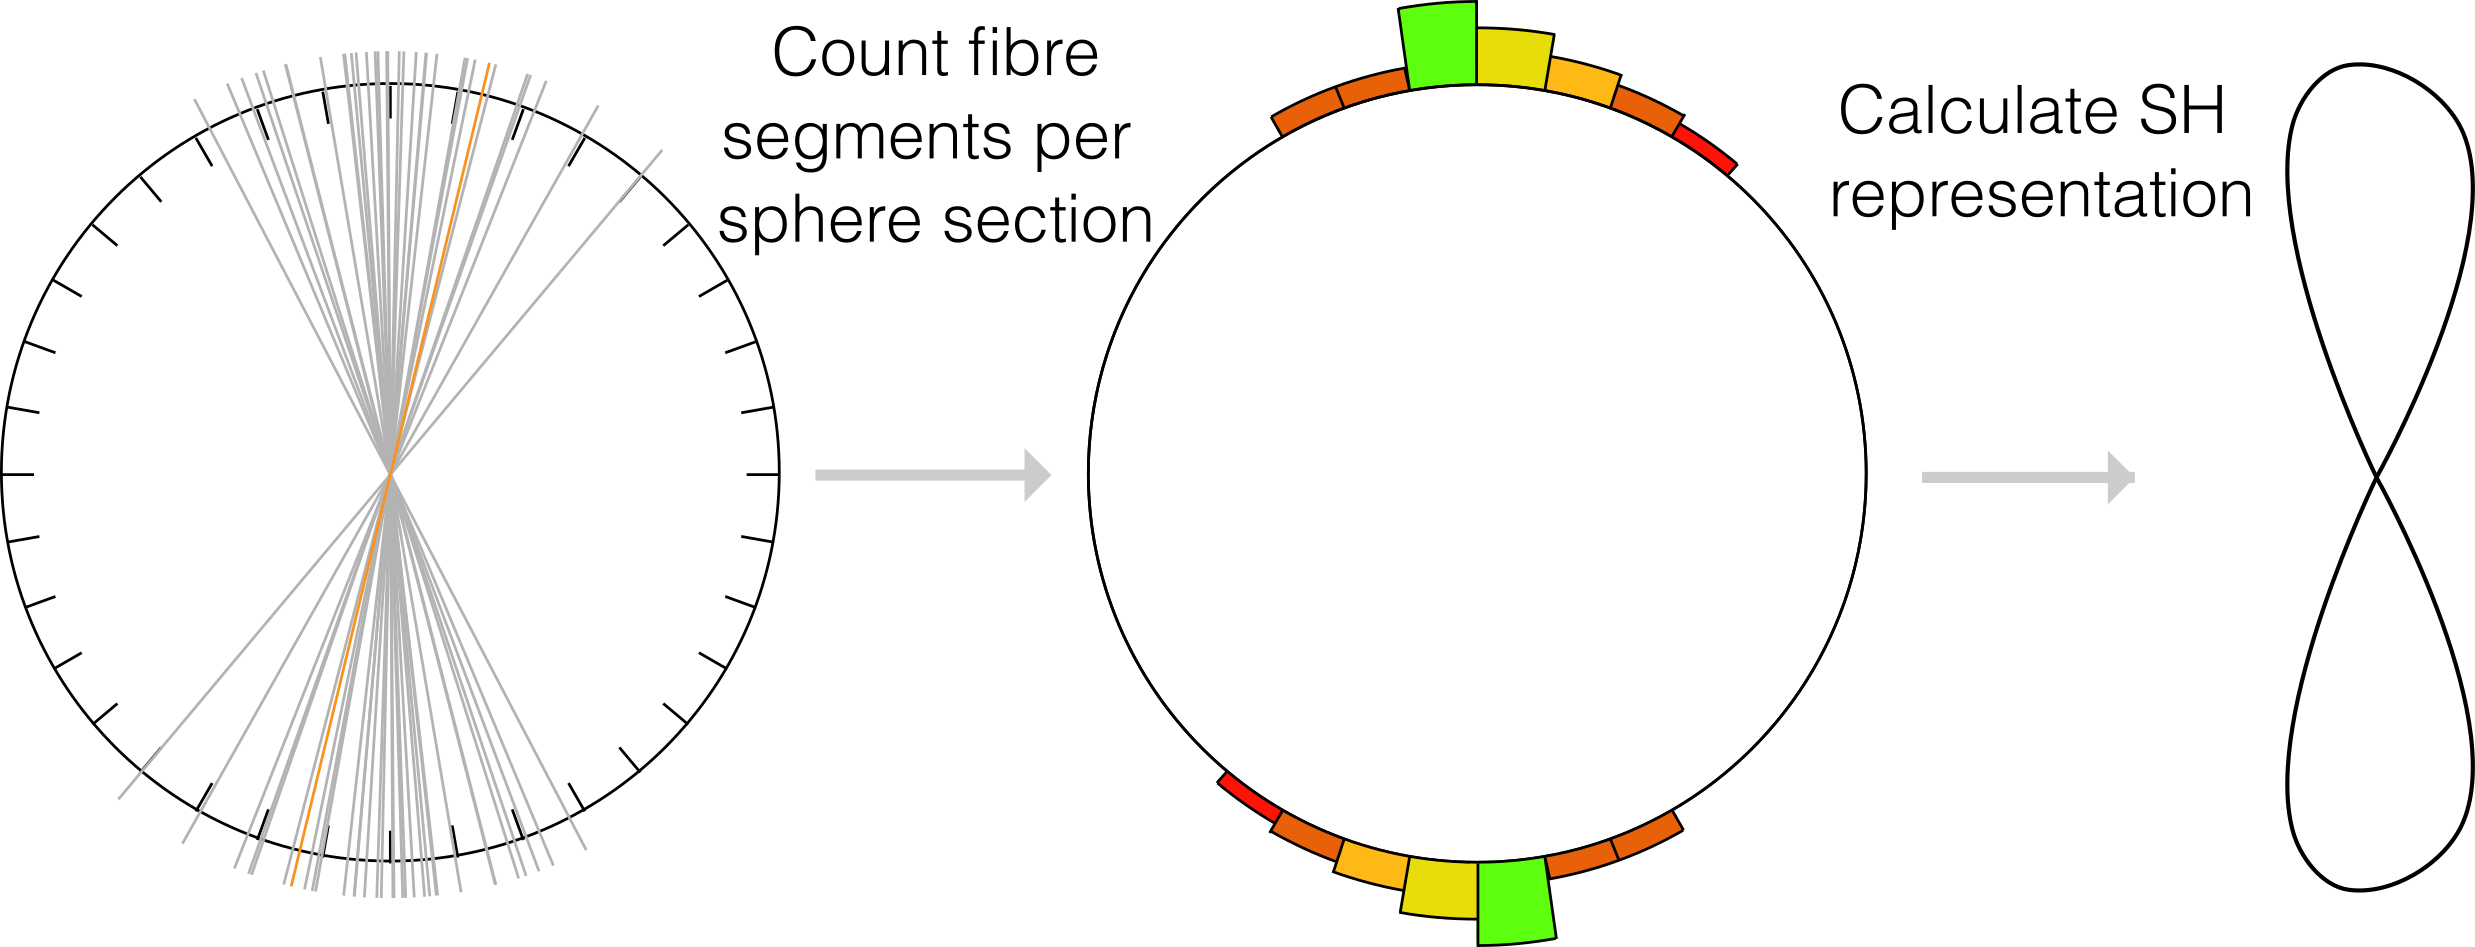
\includegraphics[width=0.8\textwidth]{figures/frf_experiment/od_estimation}
  \caption[\acs{FOD} estimation in \acs{WM} numerical phantoms]{\acs{FOD} estimation from microstructure of \ac{WM} numerical phantoms}
  \label{fig:frf_od_estimation}
\end{figure}

In order to generate a ground truth to compare with \acp{FOD} estimated from the simulated \ac{dMRI} signals, a gold standard \ac{FOD} was estimated from the \ac{WM} numerical phantom meshes.
As discussed in \Cref{sec:micro_conclusion}, it is difficult to directly compare the microstructural \ac{FOD} as seen in \Cref{fig:config_res_OD} to the \ac{SD} based \ac{FOD} since the \ac{SD} based \ac{FOD} assumes each fibre contributes to a single direction.
As an attempt to generate a microstructural \ac{FOD} comparable to that estimated from the simulated \ac{dMRI} based \acp{FOD}, the microstructural \ac{FOD} was calculated using this assumption of one direction per fibre, namely the direction that was used to align each fibre with the $z$-axis.
An alternative to this could be to split the fibre into many segments and take the mean direction of all the segments to be the fibre direction. This approach was tested, but the difference in the resulting \ac{FOD} to the proposed approach using fibre end points was minimal.

A triangulated unit sphere was used to store this \ac{FOD}, with each triangle in the sphere storing the number of fibres whose direction went through that triangle scaled by the volume of each fibre, as illustrated in \Cref{fig:frf_od_estimation}.
In order to compare this \ac{FOD} to those calculated using \ac{SD} from \ac{dMRI}, the microstructural \ac{FOD} was expanded in \aclp{SH}. A spherical function $f(\theta, \phi)$, can be expressed in terms of spherical harmonics as:
\begin{equation}
  f(\theta, \phi) = \sum_{l=0}^{\infty} \sum_{m=-l}^{l} c_l^m Y_l^m(\theta, \phi)\,,
  \label{eq:frf_SH_expansion}
\end{equation}
where
\begin{equation}
  c_l^m = \int_0^{2\pi} \int_0^\pi f(\theta, \phi) Y_l^{m*}(\theta, \phi) \sin(\theta) d\theta d\phi\,.
  \label{eq:frf_SH_coeff}
\end{equation}
$Y_l^m$ are the so-called spherical harmonics of degree $l$ and order $m$ and $*$ denotes complex conjugation.
In our case, $\theta$ and $\phi$ are discrete samples in the centre of each triangle in our unit sphere meaning one approach to finding $c_l^m$ is to turn the integral in \Cref{eq:frf_SH_coeff} into a summation. A more robust approach, however is a least squares approach \cite{Alexander2002,Brechbuhler1995} in which the spherical harmonics are re-indexed to have single index $j(l,m) = l^2 + l + m$, up to a maximum order $l_{\mathrm{max}}$.
The discrete \ac{FOD} values stored in each triangle are turned into a vector of length $n_{\mathrm{tri}}$, $\,\vec{f} = \{f(\theta_i, \phi_i), i=1,...,n\}$ and an $n_{\mathrm{tri}} \times j(l_{\mathrm{max}}, l_{\mathrm{max}})$ matrix, $X$, constructed with elements $X_{i, j(l,m)} = Y_l^m(\theta_i, \phi_i)$. Essentially, $X$ maps the SH coefficients for each $l,m$ into amplitudes along each $\theta_i, \phi_i$.
The $j(l_{\mathrm{max}}, l_{\mathrm{max}})$ vector of SH coefficients, $\vec{c}$ can then be found as
\begin{equation}
\vec{c} = (X^{*T}X)^{-1}X^{*T} \vec{f}\,.
\end{equation}

Considering the dynamics of \ac{dMRI}, the number of coefficients in $\vec{c}$ can be reduced since the \ac{FOD} is real valued and antipodally symmetric (since the \ac{dMRI} process is antipodally symmetric).
Being real valued means that the \ac{SH} coefficients exhibit conjugate symmetry (that is, $c_l^m = (-1)^mc_l^{-m*}$) \cite{Tournier2004,Alexander2002} and the antipodal symmetry means that all odd $m$ terms are 0 \cite{Alexander2002,Tournier2004}.

In order to make \acp{FOD} comparable and independent of the overall number of fibres in each phantom, each \ac{FOD} was normalised such that
\begin{equation}
  \int_0^{2\pi} \int_0^\pi f(\theta, \phi) sin(\theta) d\theta d\phi = 1\,.
  \label{frf:fod_normalisation}
\end{equation}

This normalisation also has the benefit of ensuring that the \ac{FOD} is a probability density function, describing the probability of fibre pointing in a given unit of solid angle. 



\subsection{dMRI simulation}
\label{sec:frf_dMRI_simulation}
Diffusion MRI signals were simulated from ConFiG phantoms using the Camino \ac{dMRI} simulator \cite{Cook2006,Hall2009} to perform the experiments described below. For all experiments a bulk diffusivity $D = \SI{2.0}{\micro\metre\squared\per\milli\second}$ was used in agreement with similar Monte Carlo experiments as in \Cref{sec:config_experiments} with standard Camino periodic boundaries \cite{Panagiotaki2010}.


\subsubsection{Per-fibre response function}
For each fibre 10,000 spins were initialised uniformly within the intra-axonal space and the simulations were performed using 5000 timesteps. Each phantom had $\sim 300$ fibres giving $\sim 3\times 10^6$ spins in total per phantom. A small set of test simulations were performed using 10$^5$ spins per fibre and 10$^4$ timesteps yielding negligibly different signals to these settings, so 10,000 and 5,000 were used for the main simulations for the sake of time. The measurement parameters were $\Delta = \SI{28}{\milli\second}$, $\delta = \SI{24}{\milli\second}$, $b = 0,1000,2000,\SI{3000}{\second\per\milli\metre\squared}$ and 256 gradient directions at each shell. This gives a diffusion time $d_t = \SI{20}{\milli\second}$ and $G = \SI{60}{\milli\tesla\per\metre}$ at $b = \SI{3000}{\second\per\milli\metre\squared}$, chosen to be a feasible gradient strength on a high-end clinical system.

To compare to the collection of straight fibres assumption implicit in the spherical deconvolution, an infinite cylinder representing each fibre was generated using the endpoints of each fibre to give the direction and the mean radius of the fibre as the cylinder radius. For simulation, each cylinder was aligned with the $z$-axis similarly to the ConFiG fibres so that everything was in the same space to compare the signals. The same measurement scheme was simulated in each cylinder in order to compare to the \ac{ConFiG} fibres.


\subsubsection{Extracellular contribution}
\label{sec:frf_method_extra}
To probe the contribution of the extracellular space on the overall signal, simulations were performed in \ac{ConFiG} phantoms using $10^5$ spins initialised uniformly in the space.
All fibres in the \ac{ConFiG} phantoms were treated as impermeable, meaning that the intracellular and extracellular signals could be calculated independently by labelling which compartment each spin started in. As in \Cref{sec:config_experiments}, phantoms were extended with reflected copies.

Two different measurement schemes were used to assess the contribution of the extracellular space to the overall signal. Firstly, a radial scheme with 256 measurements equally spaced in the plane perpendicular to the main fibre direction with $\delta=\SI{30}{\milli\second}, \Delta=\SI{30}{\milli\second}, r = 0, 1000, 2000, 3000, 5000, \SI{10000}{\second\per\milli\metre\squared}$ was used to assess how the extracellular signal decays in the radial direction where there should be the largest difference between intracellular and extracellular signals as in Raffelt et al. \cite{Raffelt2012}. Additionally, a scheme with the same b-values but directions equidistributed across the sphere was used to test how the signal varies in all directions.


In each case, simulations were also performed in a phantom of straight parallel cylinders with radii matching the radii in the $\kappa=100$ phantom.

\subsection{Signal analysis}
\label{sec:frf_signal_analysis}
Throughout this work, \ac{SH} representations of signals are used. The MATLAB implementation of \ac{CSD} \cite{Tournier2007} from J-Donald Tournier (\url{https://github.com/jdtournier/csd}) is used to calculate \ac{SH} decompositions of signals. This is the same technique as used in popular \ac{dMRI} tractography tool MRtrix3 \cite{Tournier2019} and follows the procedure outlined in \Cref{sec:frf_true_frf_extraction} for \ac{SH} decomposition of the \ac{dMRI} signal, where $\theta, \phi$ are the gradient directions.
\begin{figure}
  \centering
 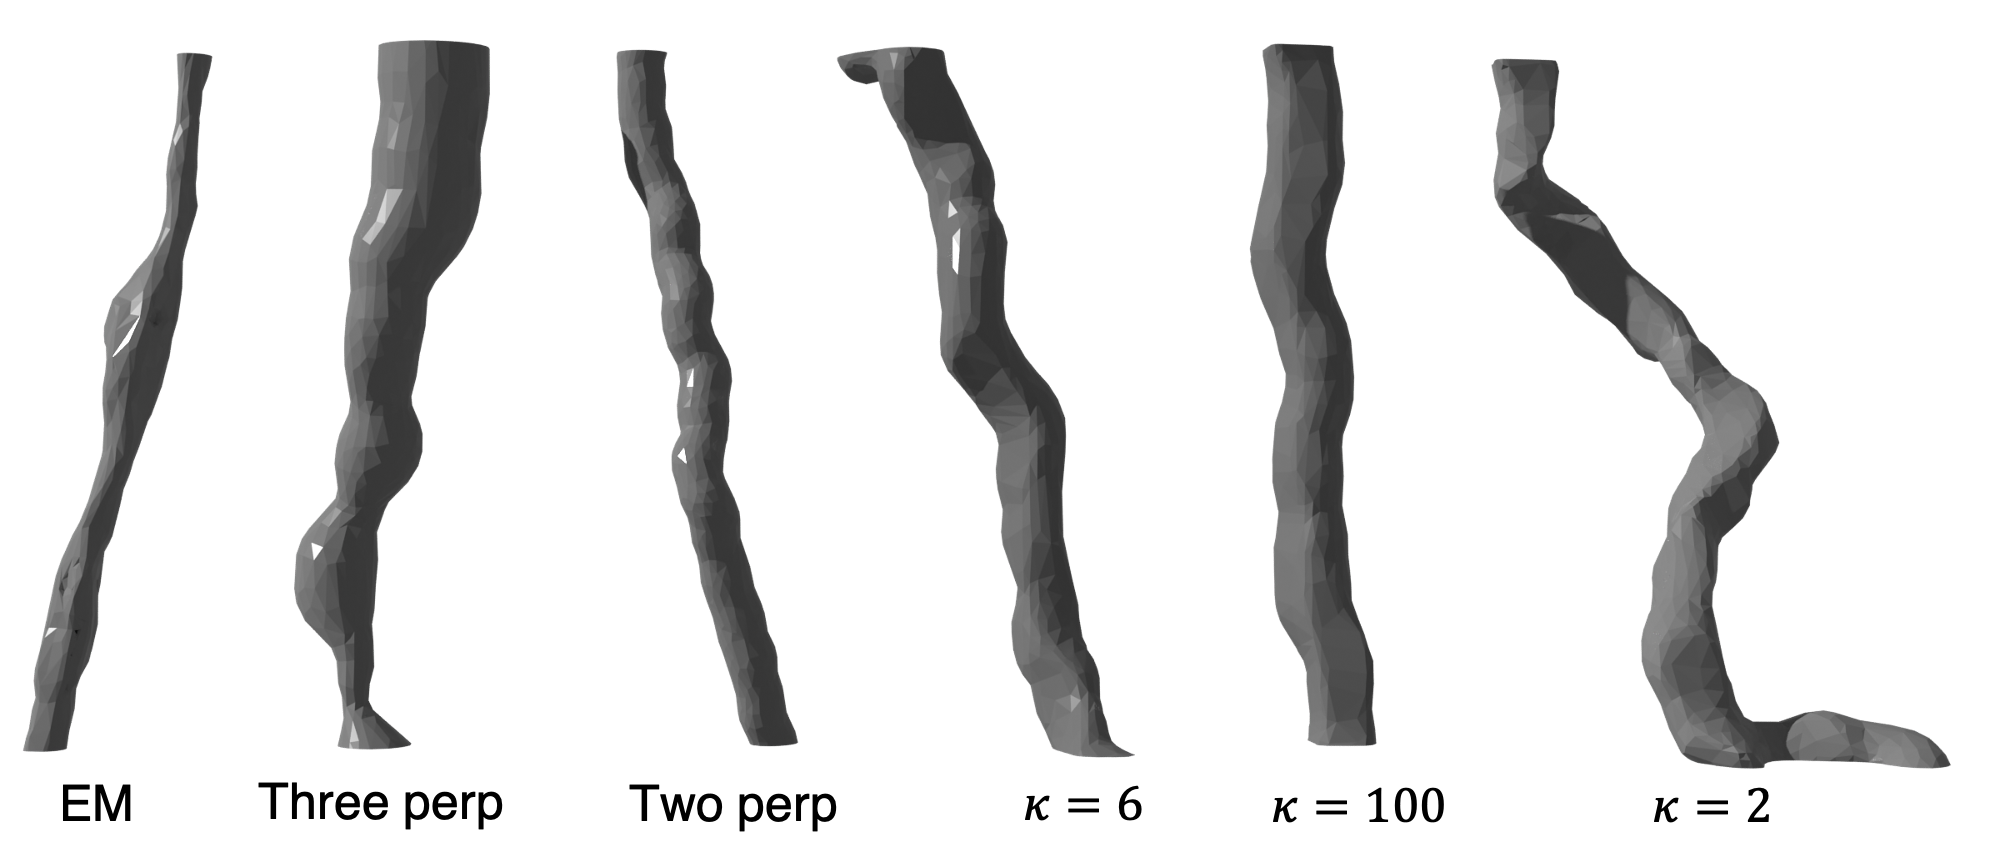
\includegraphics[width=\textwidth]{figures/frf_experiment/fibre_examples_caption}
  \caption[Example fibres used in the per-fibre response function experiments]{Example fibres used in the per-fibre response function experiments. Left to right: Real EM, Three crossing bundles, Two crossing bundles, $\kappa=6, \kappa=100, \kappa=2$.}
  \label{fig:frf_example_fibres}
\end{figure}
\subsubsection{Per-fibre response function}
\label{sec:frf_sig_proc_per_fibre}
Since the individual axons have been aligned with the $z$-axis, the signals from each fibre can be directly compared with one another as the gradient directions are aligned with respect to each fibre.
For each numerical phantom the median, 10th and 90th percentile of the signal in each direction at each b-value across all the axons in the phantom were calculated.

To assess how much of an impact any variation in the per-fibre response function may have on the \ac{FOD} estimation, the per-fibre signals were rotated to align with the original fibre direction and the volume-weighted mean signal calculated for each phantom. This mean signal was used to estimate the \ac{FOD} using an \ac{FRF} based on the median, 10th and 90th percentile signal from each phantom using \ac{CSD} \cite{Tournier2019,Tournier2007}. In order to better compare against the gold standard \ac{FOD} calculated from the microstructure (\Cref{sec:frf_true_frf_extraction}), the resulting \ac{FOD} was normalised to integrate to one using \Cref{frf:fod_normalisation}.

\subsubsection{Extracellular contribution}
\label{sec:frf_sig_proc_extra}
For the radial simulations, the mean radial signal at each b-value was calculated for each of the compartments (intracellular, extracellular and total space). For the simulations in all directions, the spherical harmonic representation of the signal was calculated for each of the compartments at each b-value.

As in the per-fibre response function experiment, the impact of the variation in signals between intracellular-only and total signals on the \ac{FOD} was investigate. The \ac{FRF} was calculated from the intracellular-only signal and total signal and each were used to estimate the \ac{FOD} from the total signals. In some sense, this experiment can be seen as testing the `ideal' \ac{FRF} from the intra-axonal signal only which we ideally wish to obtain against the `practical' \ac{FRF} from the total signal (including extra-axonal contributions) which we obtain in practice.


\section{Results}
\label{sec:frf_results}


\subsection{Per-fibre response function}
\label{sec:frf_res_per_fibre}
\Cref{fig:frf_example_fibres} shows a set of example fibres from the phantoms used in this experiment, demonstrating the complex morphology that ConFiG fibres can have as well as the kind of thing we see in real fibres.

This morphological variation in the fibres causes the \ac{dMRI} signal response per-fibre to vary as can be seen in \Cref{fig:frf_prctiles_kappa_b2000}, which shows the median, 10th and 90th percentile signals across all fibres in each phantom at $b=\SI{2000}{\second\per\milli\metre\squared}$.
The variation in the response function depends on the complexity of the fibre arrangement, with the most complex three crossing bundle arrangement leading to the largest variation in response functions.

This variation in the \ac{FRF} is seen across each $b$-value from $1000$ to $\SI{3000}{\second\per\milli\metre\squared}$ as demonstrated in \Cref{fig:frf_prctiles_b123} for the $\kappa=2$, three crossing and EM fibre phantoms, chosen since these display the most variation for each phantom category.


\begin{figure}[h!]
  \centering
  \begin{subfigure}[]{0.4\textwidth}
    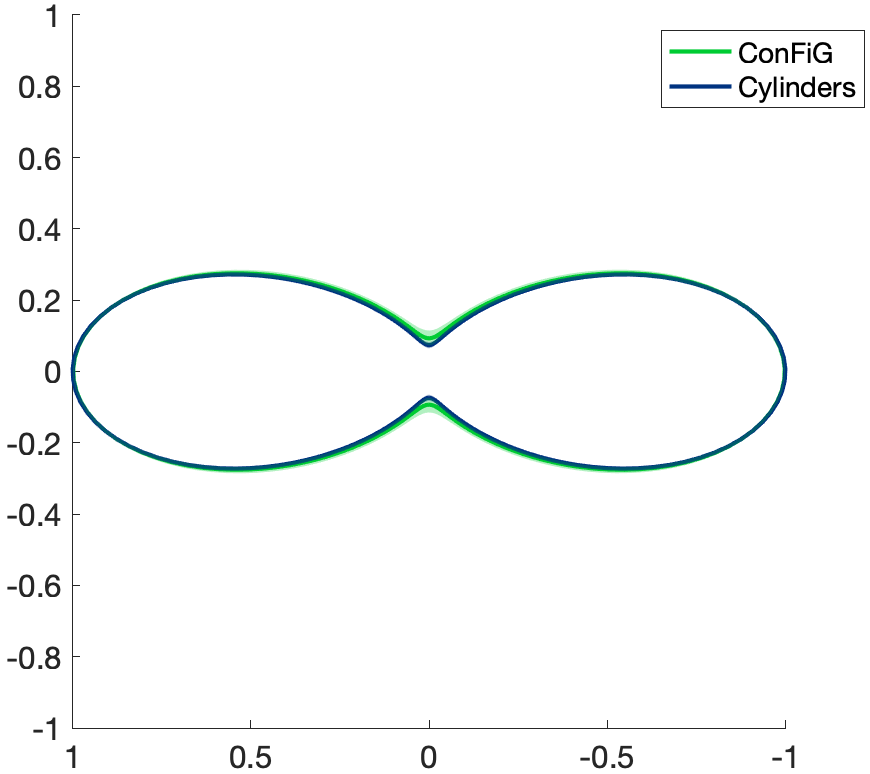
\includegraphics[width=\textwidth]{figures/frf_experiment/fibres_prctiles_kappa_100_b_2000.png}
    \caption{$\kappa = 100$}
  \end{subfigure}
  ~
  \begin{subfigure}[]{0.4\textwidth}
    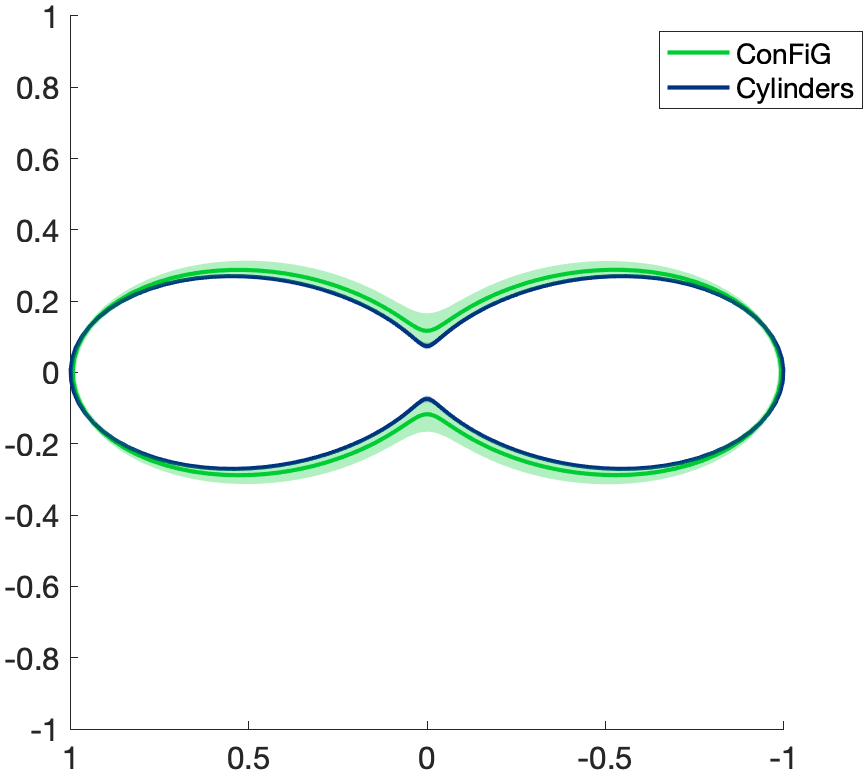
\includegraphics[width=\textwidth]{figures/frf_experiment/fibres_prctiles_kappa_6_b_2000.png}
    \caption{$\kappa = 6$}
  \end{subfigure}

  \begin{subfigure}[]{0.4\textwidth}
    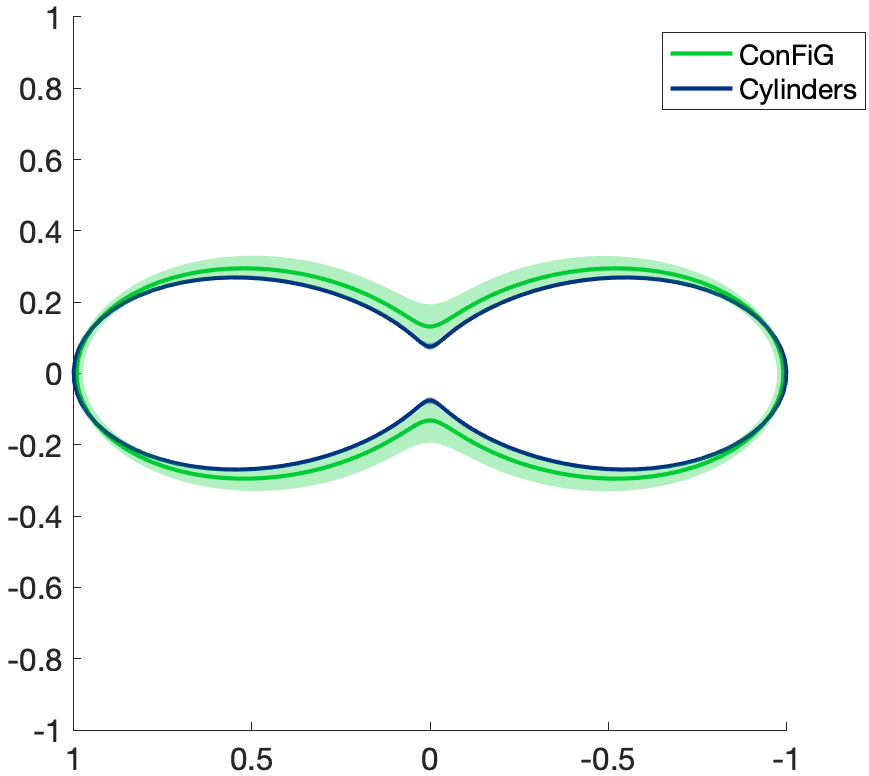
\includegraphics[width=\textwidth]{figures/frf_experiment/fibres_prctiles_kappa_2_b_2000.png}
    \caption{$\kappa = 2$}
  \end{subfigure}
  ~
  \begin{subfigure}[]{0.4\textwidth}
    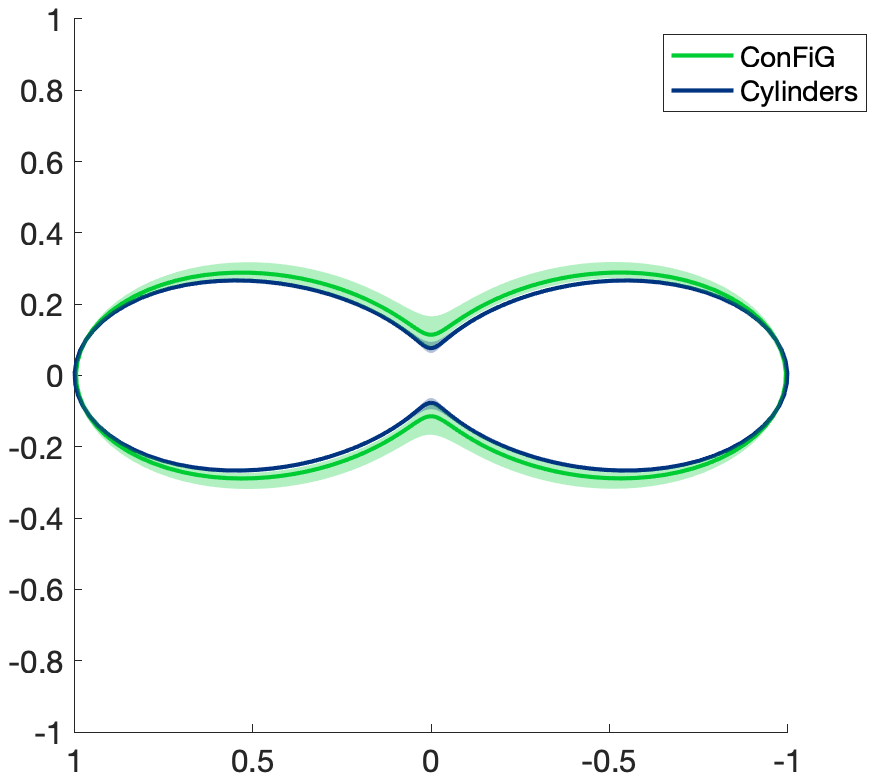
\includegraphics[width=\textwidth]{figures/frf_experiment/twoperp_prctiles_b_2000.png}
    \caption{Two crossing}
  \end{subfigure}

  \begin{subfigure}[]{0.4\textwidth}
    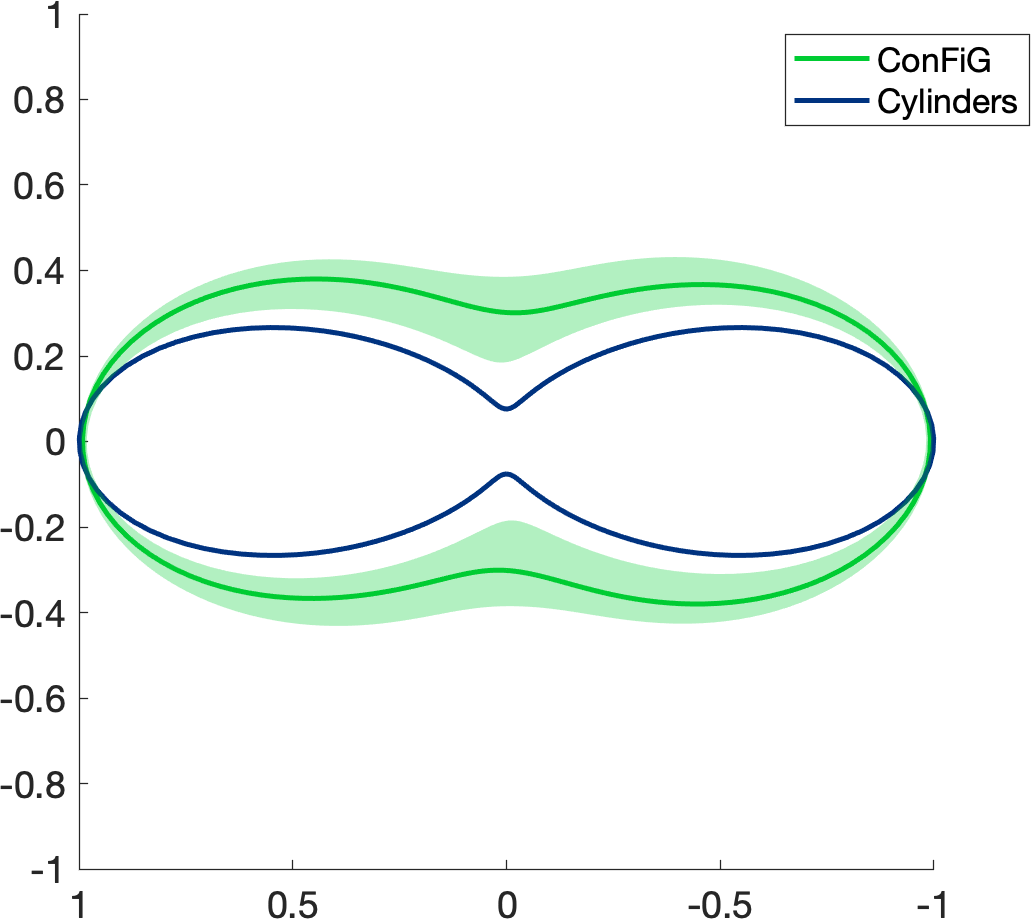
\includegraphics[width=\textwidth]{figures/frf_experiment/threeperp_prctiles_b_2000.png}
    \caption{Three crossing}
  \end{subfigure}
  ~
  \begin{subfigure}[]{0.4\textwidth}
    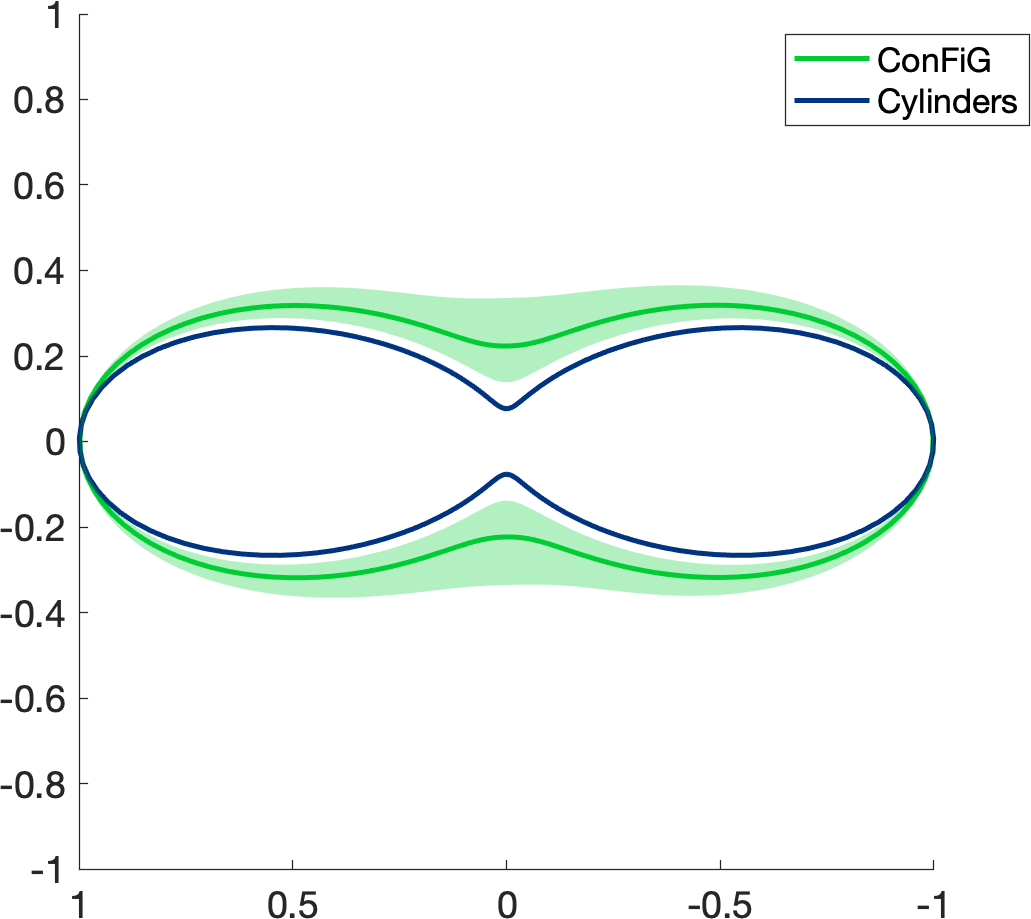
\includegraphics[width=\textwidth]{figures/frf_experiment/EMfibres_prctiles_b_2000.png}
    \caption{\ac{EM} fibres}
  \end{subfigure}

  \caption[Per-fibre FRF at $b=\SI{2000}{\second\per\milli\metre\squared}$]{Per-fibre FRF at $b = \SI{2000}{\second\per\milli\metre\squared}$ for the range of phantoms used in this experiment showing the variability in response function across fibres. Solid line shows mean signal and shaded area shows 5th and 95th percentiles. }
  \label{fig:frf_prctiles_kappa_b2000}
\end{figure}


\begin{figure}
  \centering
  \begin{subfigure}[]{\textwidth}
  \begin{subfigure}[]{0.3\textwidth}
    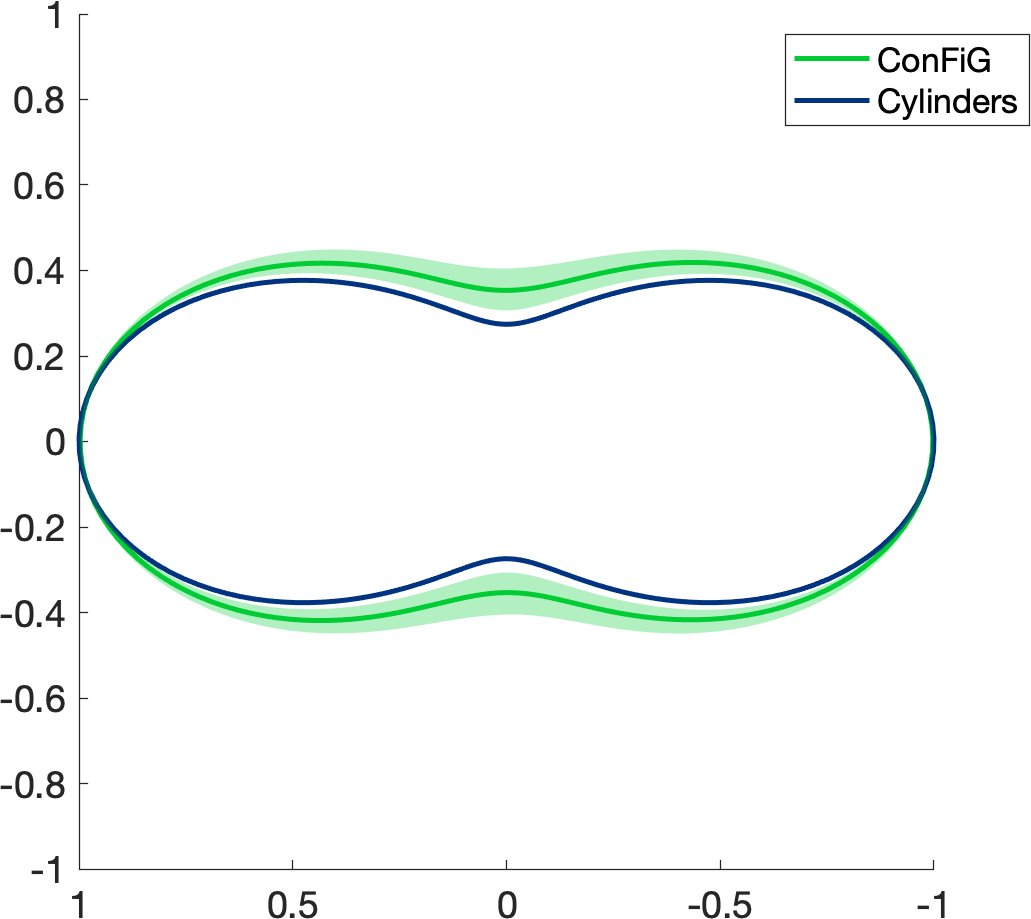
\includegraphics[width=\textwidth]{figures/frf_experiment/fibres_prctiles_kappa_2_b_1000}
  \end{subfigure}
  ~
  \begin{subfigure}[]{0.3\textwidth}
    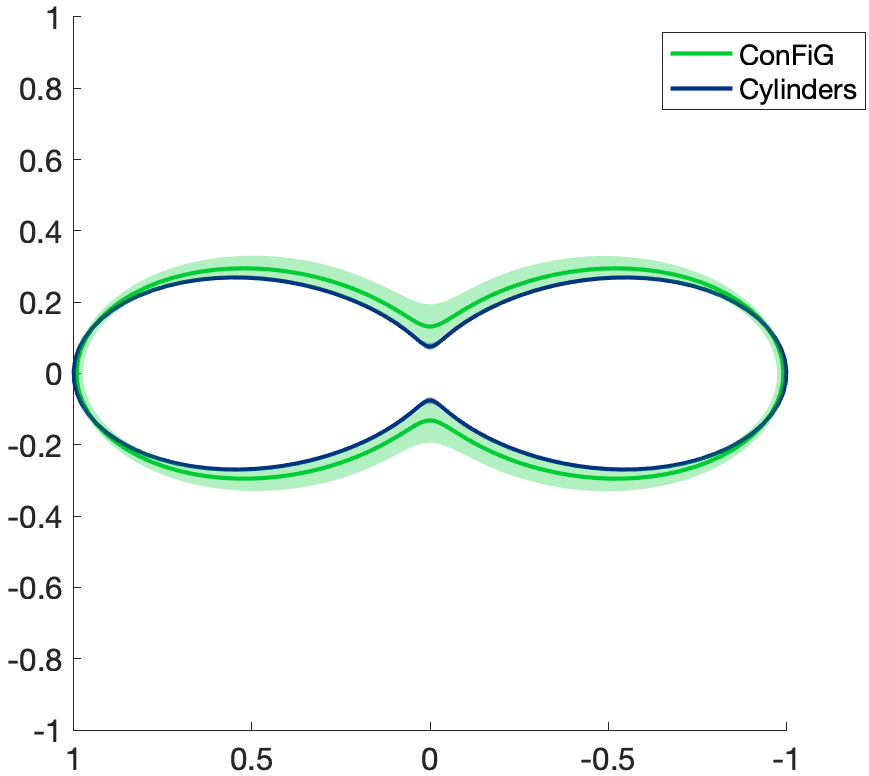
\includegraphics[width=\textwidth]{figures/frf_experiment/fibres_prctiles_kappa_2_b_2000}
  \end{subfigure}
  ~
  \begin{subfigure}[]{0.3\textwidth}
    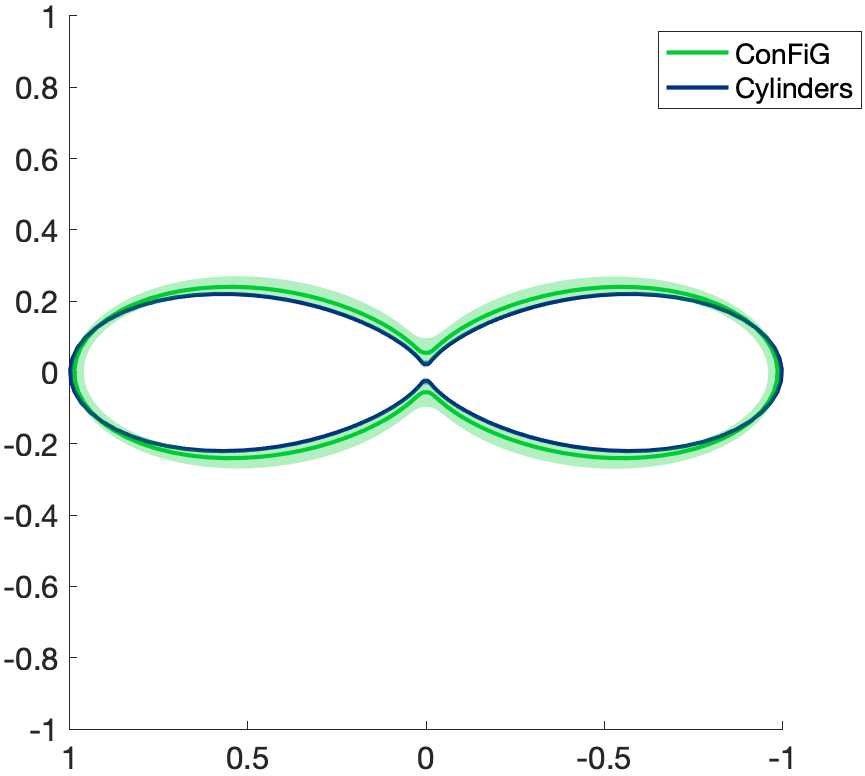
\includegraphics[width=\textwidth]{figures/frf_experiment/fibres_prctiles_kappa_2_b_3000}
  \end{subfigure}
  \caption{$\kappa = 2$}
  \end{subfigure}

  \begin{subfigure}[]{\textwidth}
  \begin{subfigure}[]{0.3\textwidth}
    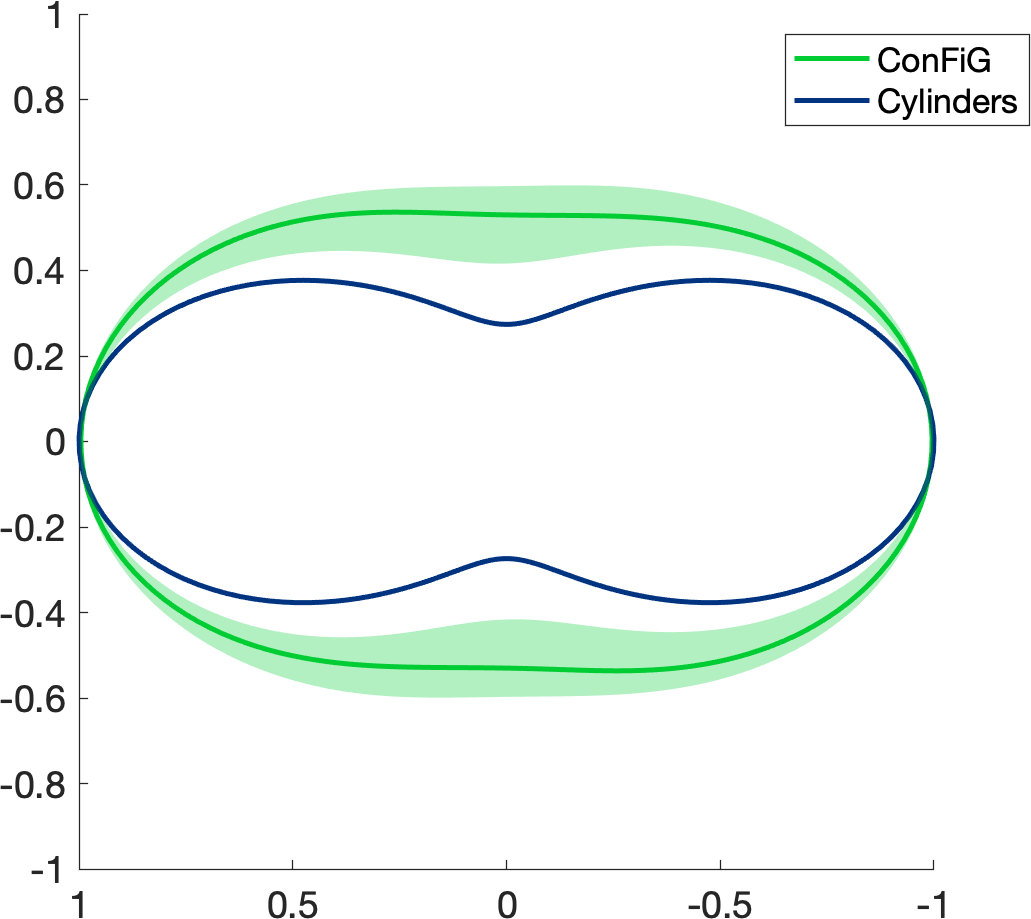
\includegraphics[width=\textwidth]{figures/frf_experiment/threeperp_prctiles_b_1000}
  \end{subfigure}
  ~
  \begin{subfigure}[]{0.3\textwidth}
    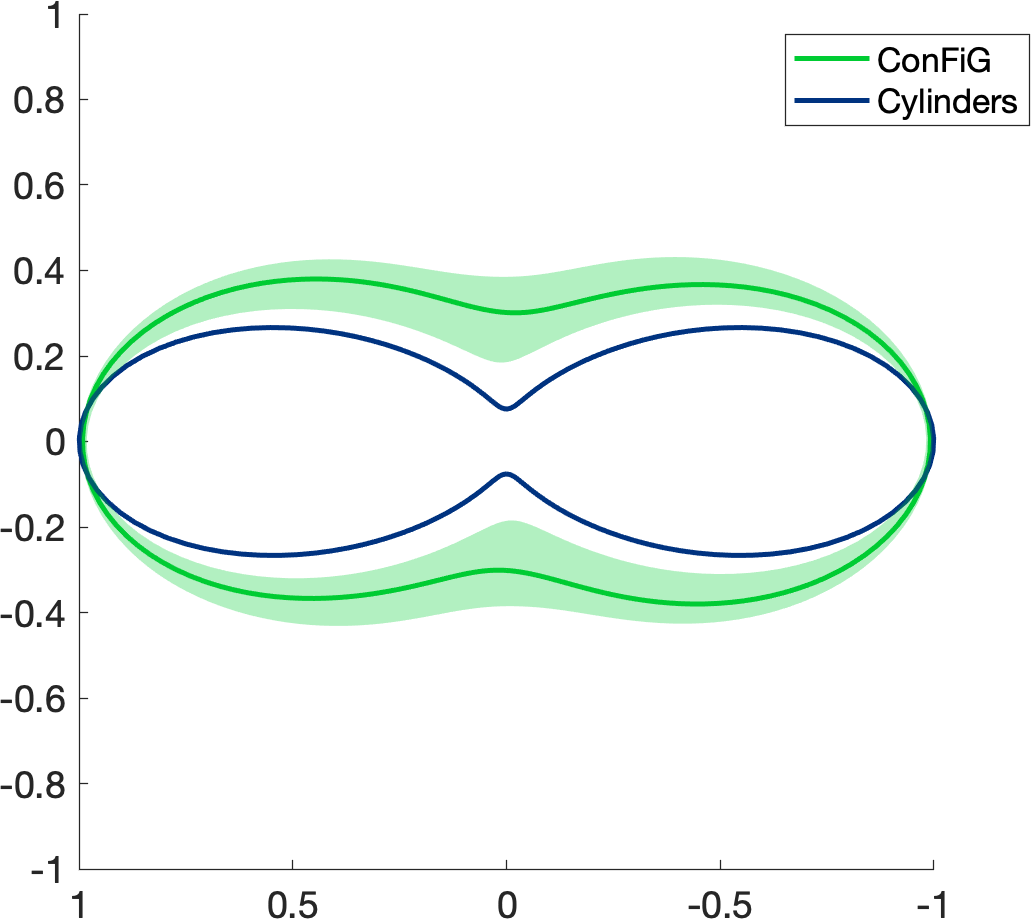
\includegraphics[width=\textwidth]{figures/frf_experiment/threeperp_prctiles_b_2000}
  \end{subfigure}
  ~
  \begin{subfigure}[]{0.3\textwidth}
    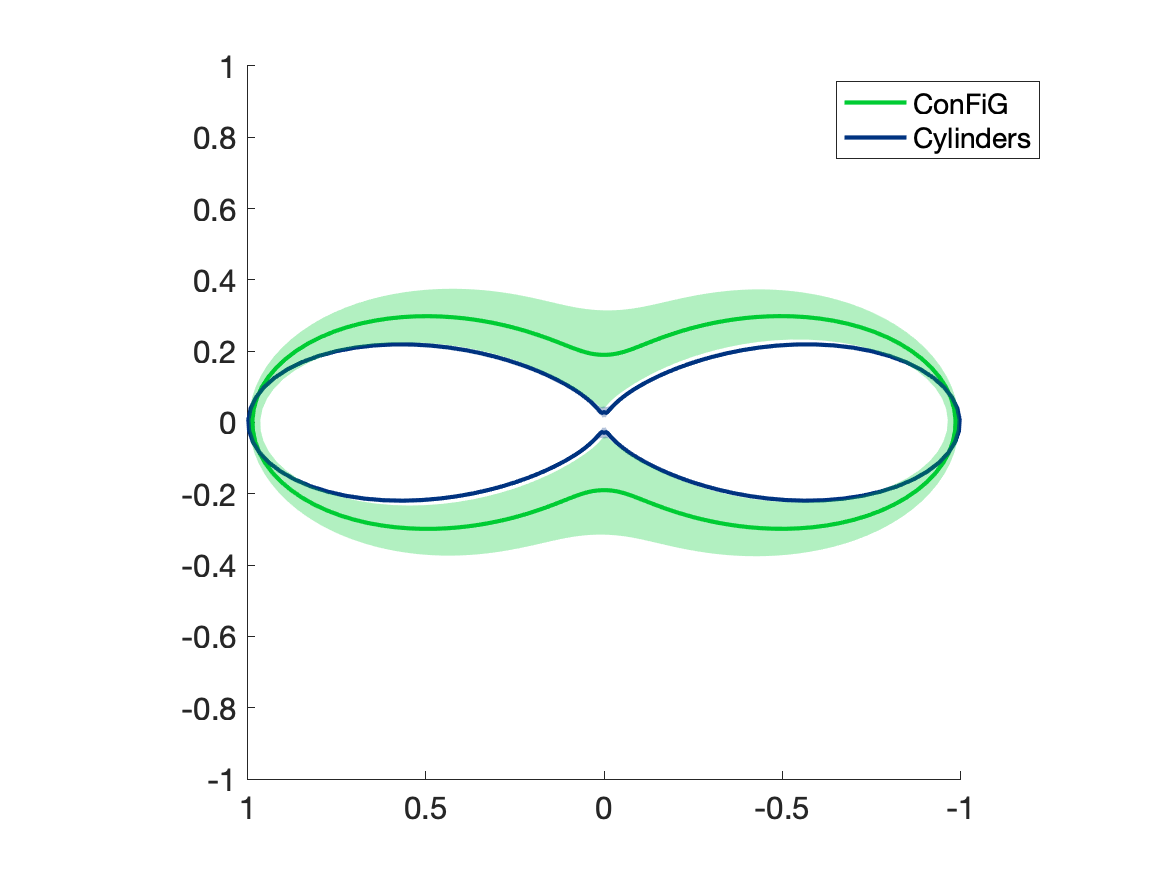
\includegraphics[width=\textwidth]{figures/frf_experiment/threeperp_prctiles_b_3000}
  \end{subfigure}
  \caption{Three crossing}
  \end{subfigure}

  \begin{subfigure}[]{\textwidth}
  \begin{subfigure}[]{0.3\textwidth}
    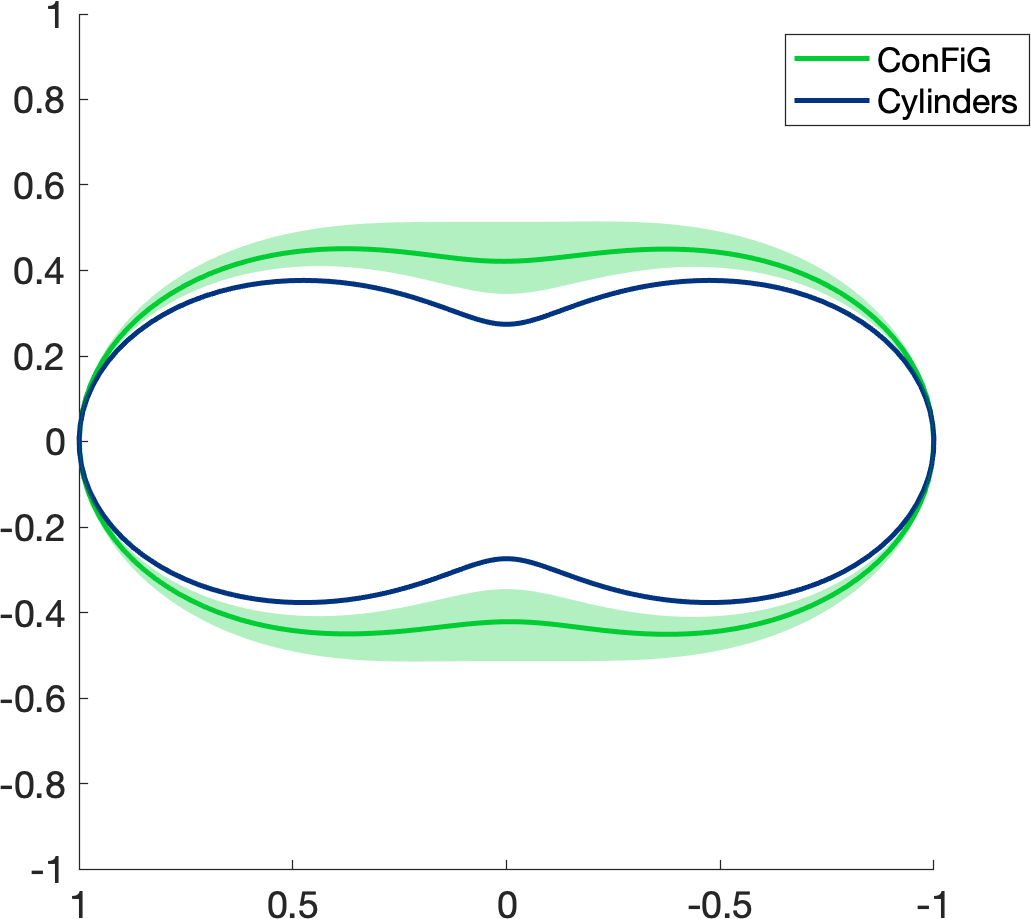
\includegraphics[width=\textwidth]{figures/frf_experiment/EMfibres_prctiles_b_1000}
    \caption*{$b=\SI{1000}{\second\per\milli\metre\squared}$}
  \end{subfigure}
  ~
  \begin{subfigure}[]{0.3\textwidth}
    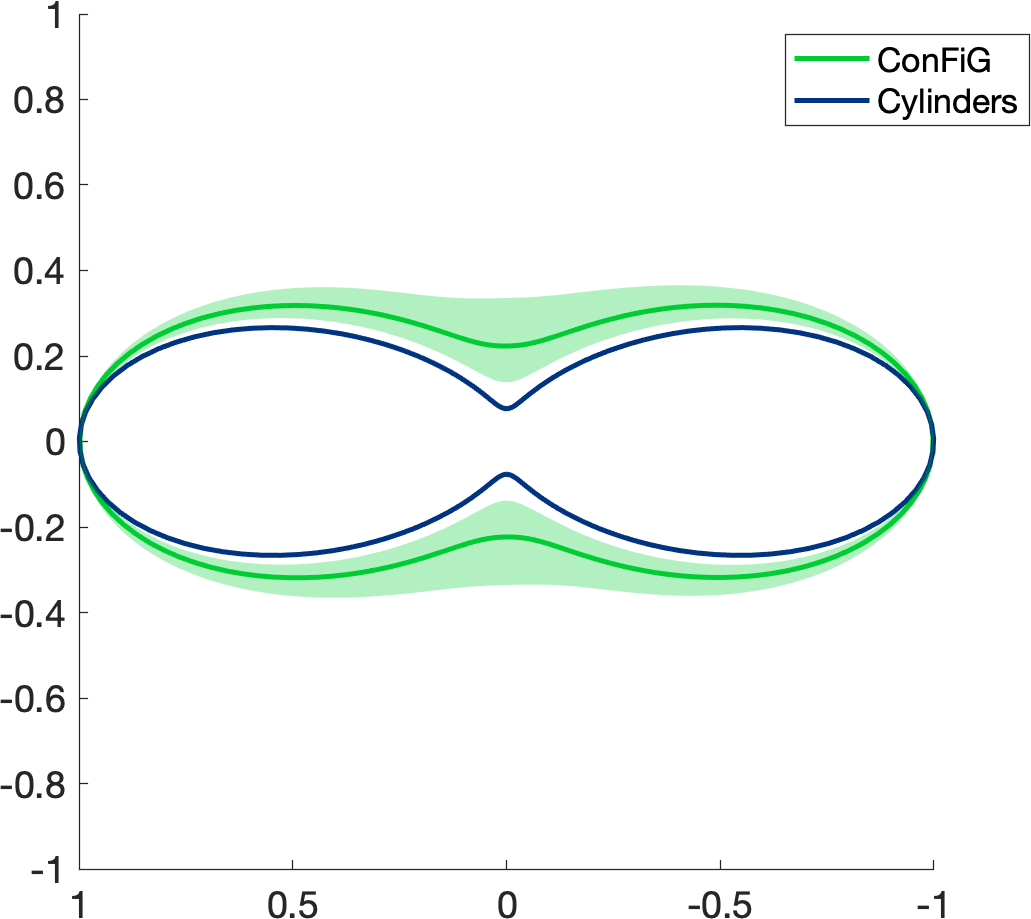
\includegraphics[width=\textwidth]{figures/frf_experiment/EMfibres_prctiles_b_2000}
    \caption*{$b=\SI{2000}{\second\per\milli\metre\squared}$}
  \end{subfigure}
  ~
  \begin{subfigure}[]{0.3\textwidth}
    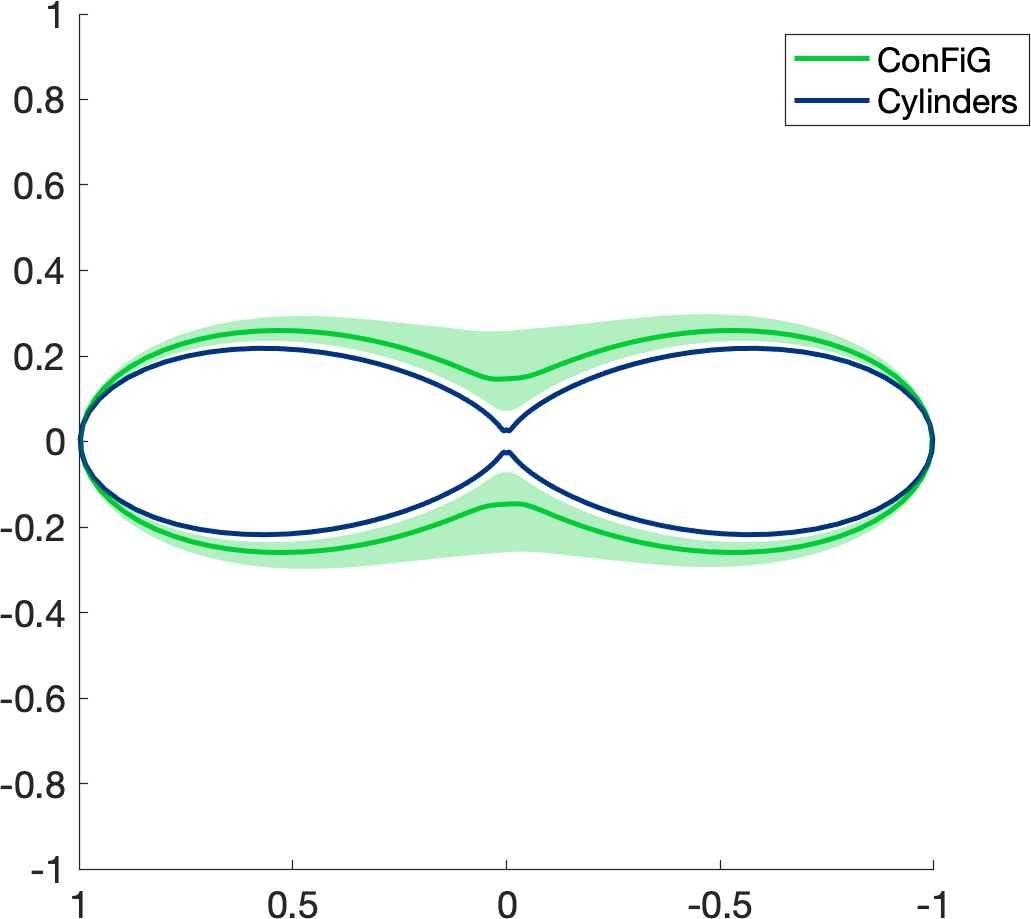
\includegraphics[width=\textwidth]{figures/frf_experiment/EMfibres_prctiles_b_3000}
    \caption*{$b=\SI{3000}{\second\per\milli\metre\squared}$}
  \end{subfigure}
  \caption{EMfibres}
  \end{subfigure}
  \caption[Per-fibre response function at $b = 1000,2000,\SI{3000}{\second\per\milli\metre\squared}$]{Per-fibre response function at $b = 1000,2000,\SI{3000}{\second\per\milli\metre\squared}$ (left-to-right) for (a) the $\kappa=2$ phantom, (b) the three crossing phantom and (c) the EM fibres.}
  \label{fig:frf_prctiles_b123}
\end{figure}

\begin{comment}
\begin{figure}
  \centering
  \begin{subfigure}[]{0.4\textwidth}
    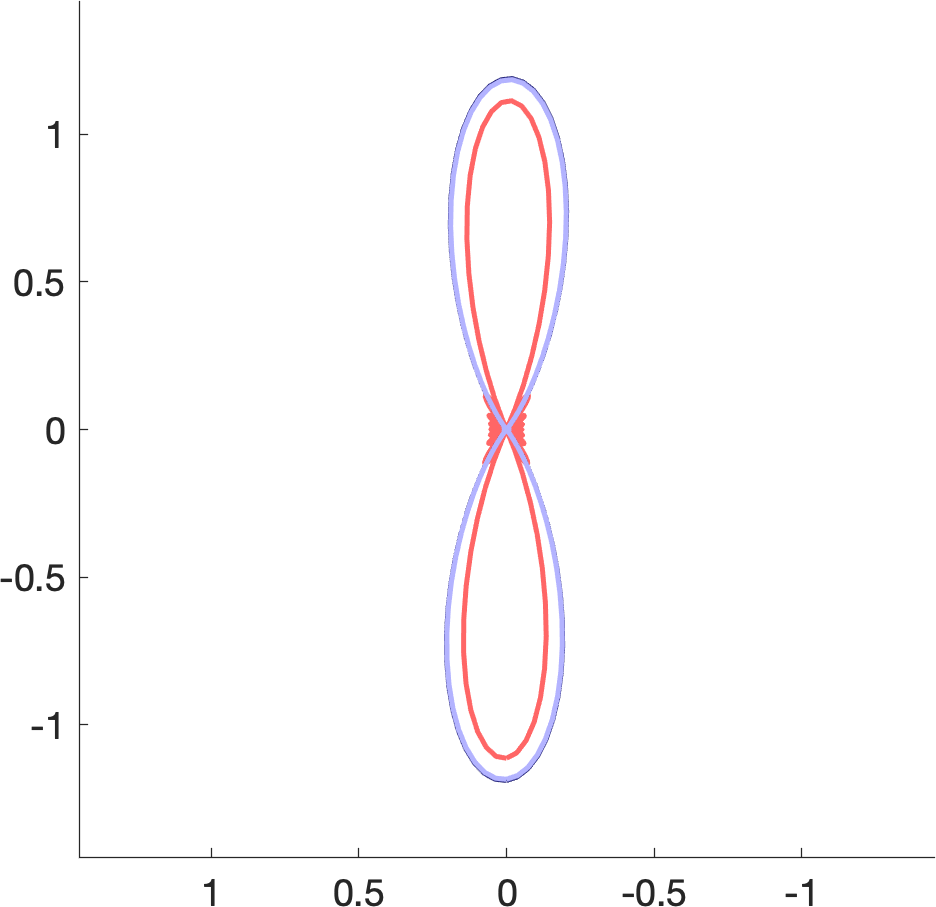
\includegraphics[width=\textwidth]{figures/frf_experiment/fibres_fod_kappa100_b_3000.png}
    \caption{$\kappa = 100$}
  \end{subfigure}
  ~
  \begin{subfigure}[]{0.4\textwidth}
    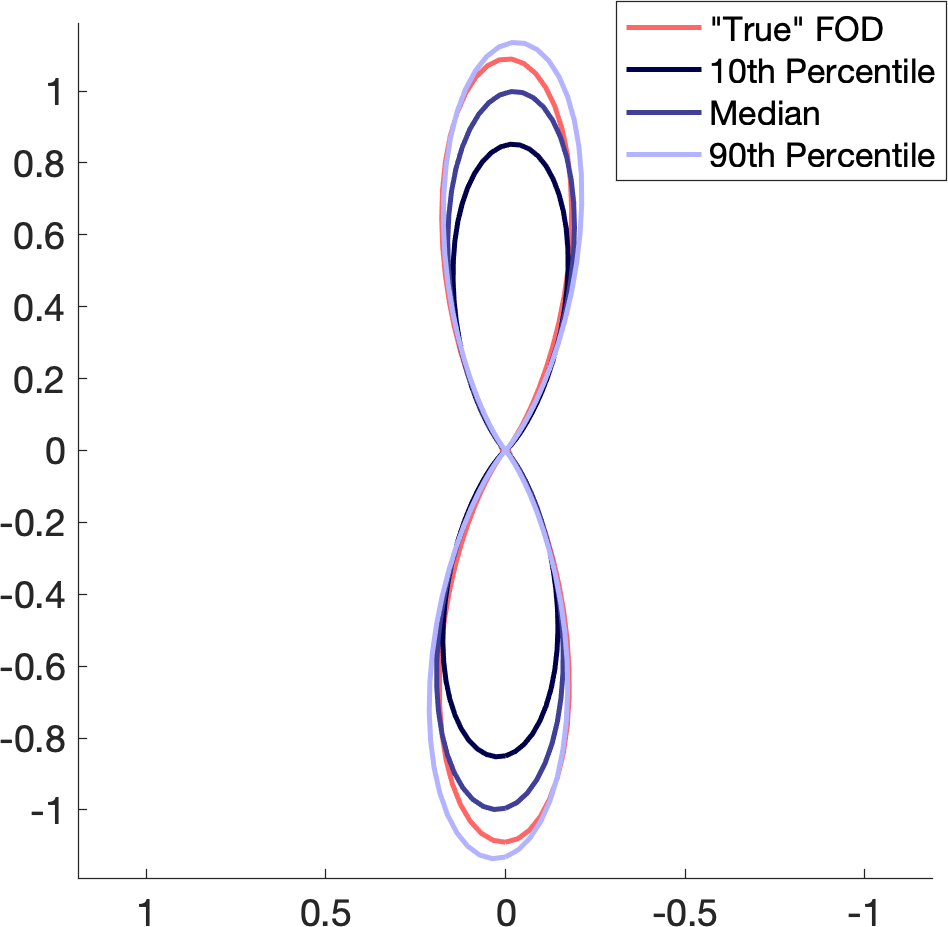
\includegraphics[width=\textwidth]{figures/frf_experiment/fibres_fod_kappa6_b_3000_leg.png}
    \caption{$\kappa = 6$}
  \end{subfigure}

  \begin{subfigure}[]{0.4\textwidth}
    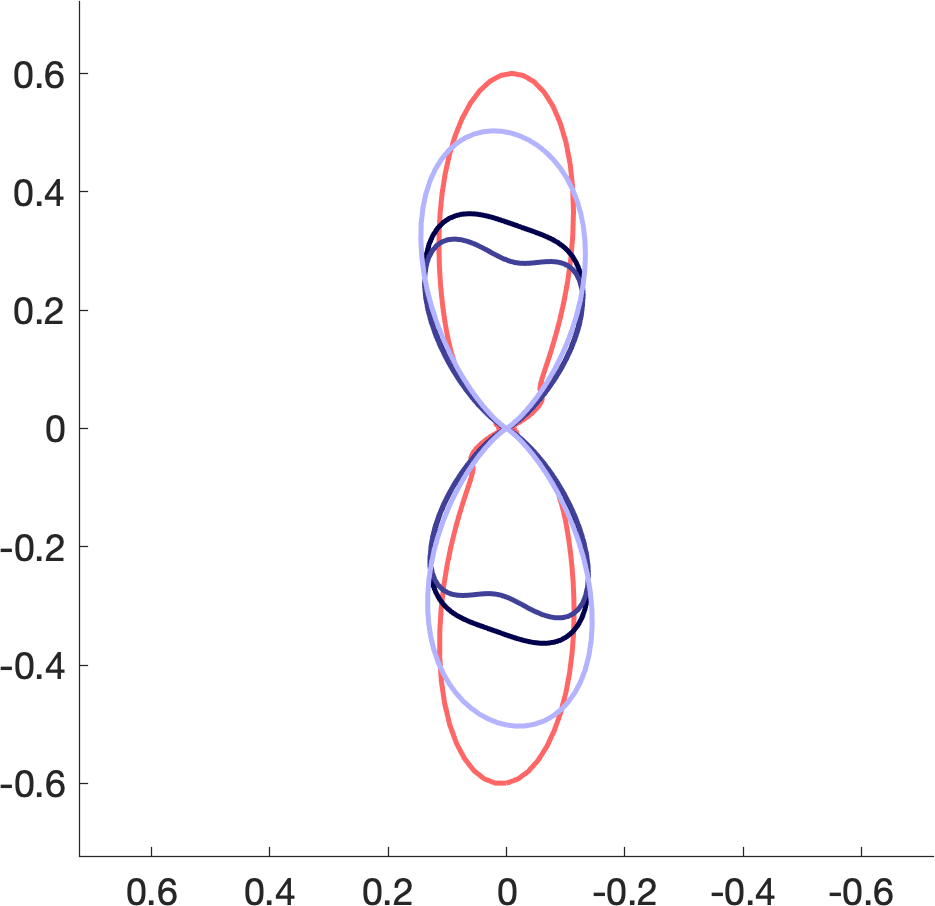
\includegraphics[width=\textwidth]{figures/frf_experiment/fibres_fod_kappa2_b_3000.png}
    \caption{$\kappa = 2$}
  \end{subfigure}
  ~
  \begin{subfigure}[]{0.4\textwidth}
    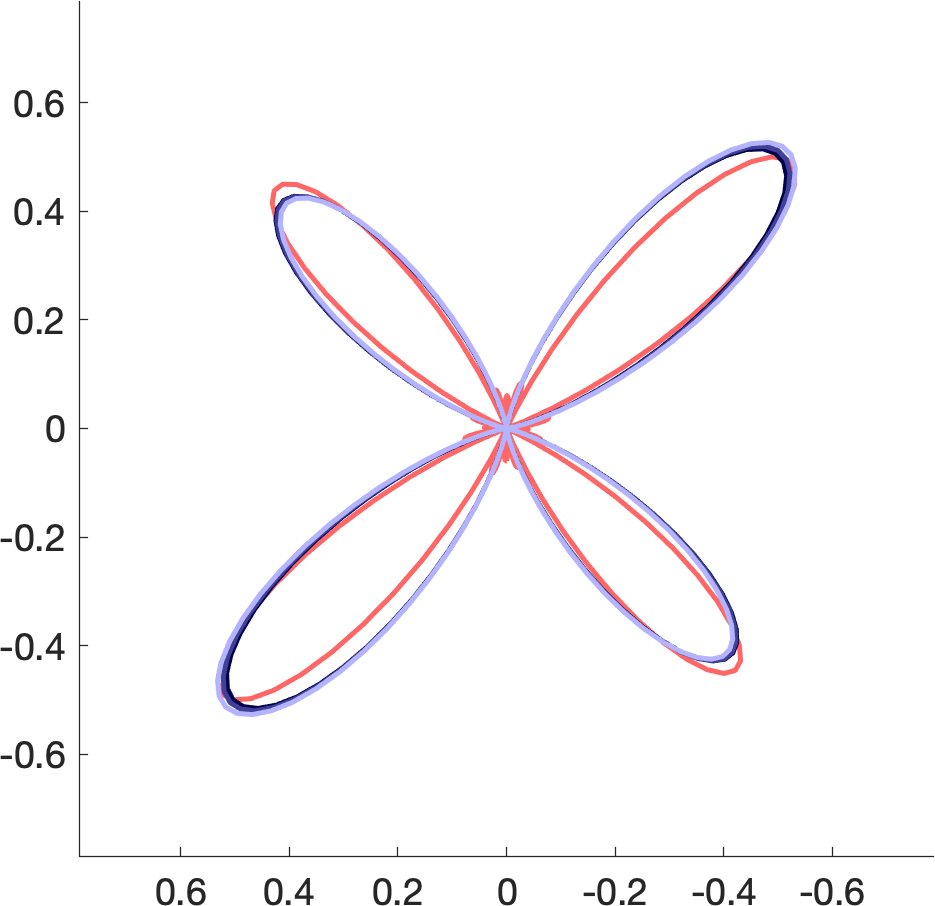
\includegraphics[width=\textwidth]{figures/frf_experiment/twoperp_fod_b_3000.png}
    \caption{Two crossing}
  \end{subfigure}

  \begin{subfigure}[]{0.4\textwidth}
    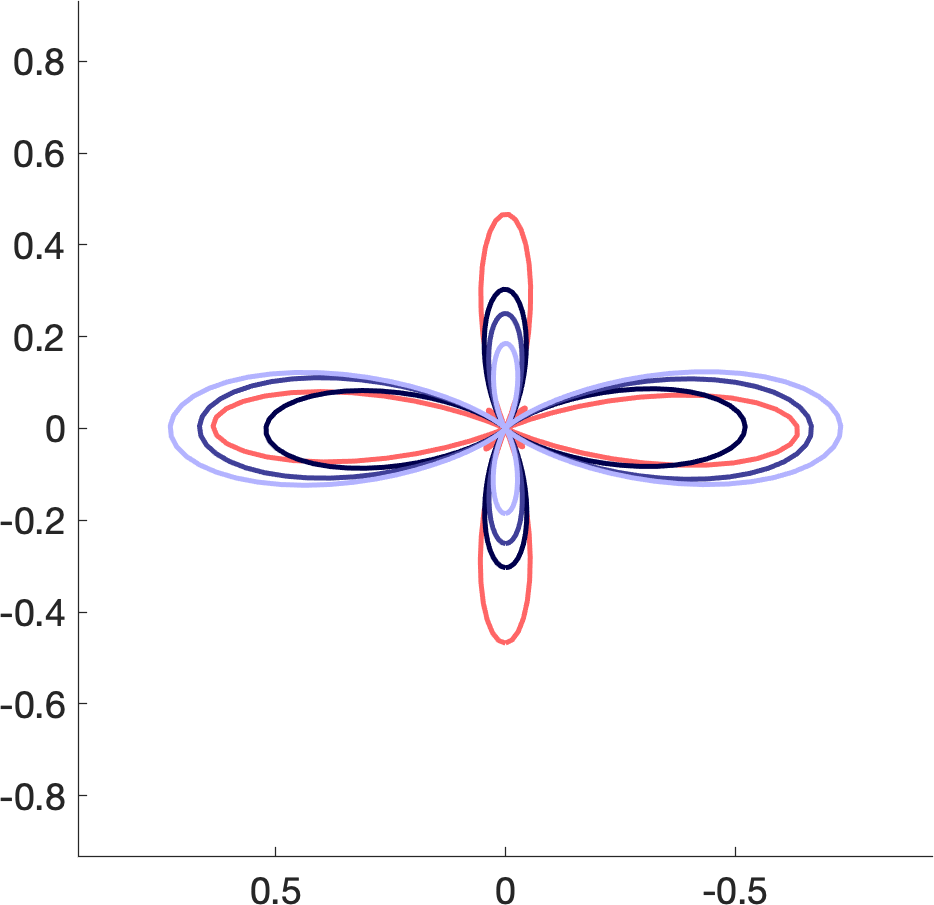
\includegraphics[width=\textwidth]{figures/frf_experiment/threeperp_fod_b_3000.png}
    \caption{Three crossing}
  \end{subfigure}
  ~
  \begin{subfigure}[]{0.4\textwidth}
    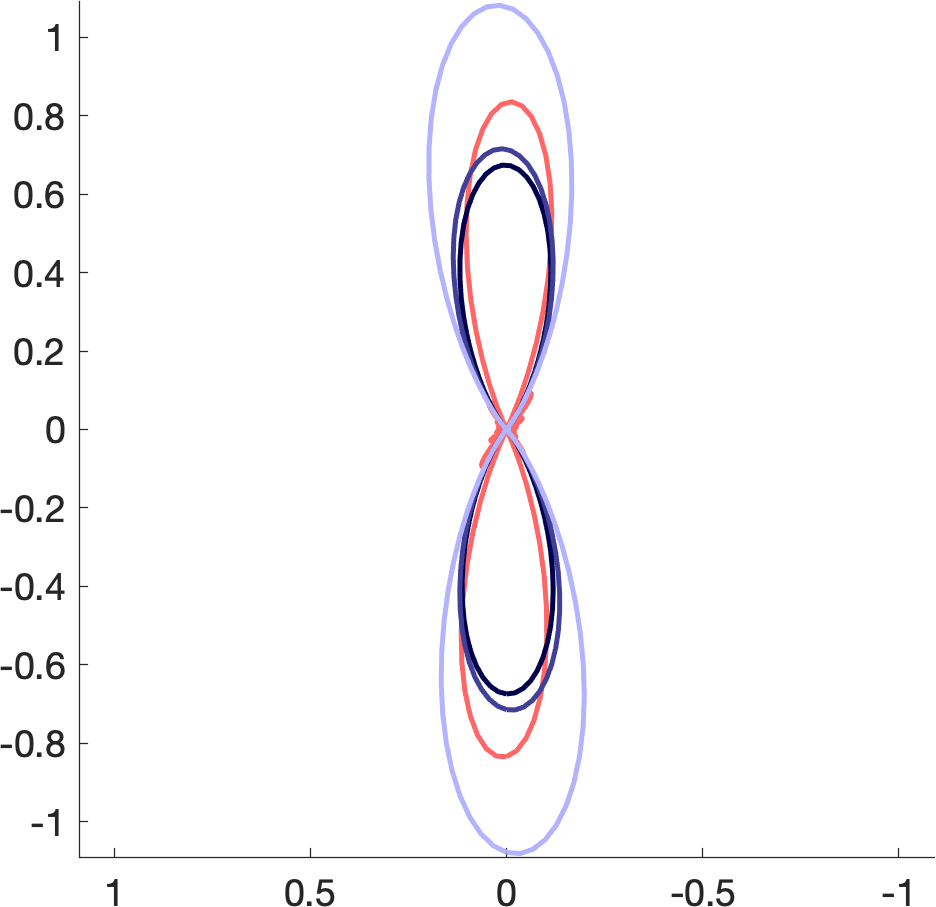
\includegraphics[width=\textwidth]{figures/frf_experiment/EMfibres_fod_b_3000.png}
    \caption{\ac{EM} fibres}
  \end{subfigure}

  \caption[Imapct of the FRF variability on FOD estimation]{Variations in the \ac{FOD} estimated using the 10th percentile, 90th percentile and median signal for the \ac{FRF} for a range of phantoms.}
  \label{fig:frf_fod_kappa_b2000}
\end{figure}
\end{comment}

\begin{figure}
  \centering
  \makebox[\textwidth][c]{
  \begin{minipage}[c]{0.15\textwidth}
    \subcaption{$\kappa = 100$}
  \end{minipage}
  \hfill
  \begin{minipage}[c]{1\textwidth}
  % \begin{subfigure}[]{1\textwidth}
  \begin{subfigure}[]{0.245\textwidth}
    \caption*{Gold standard FOD}
    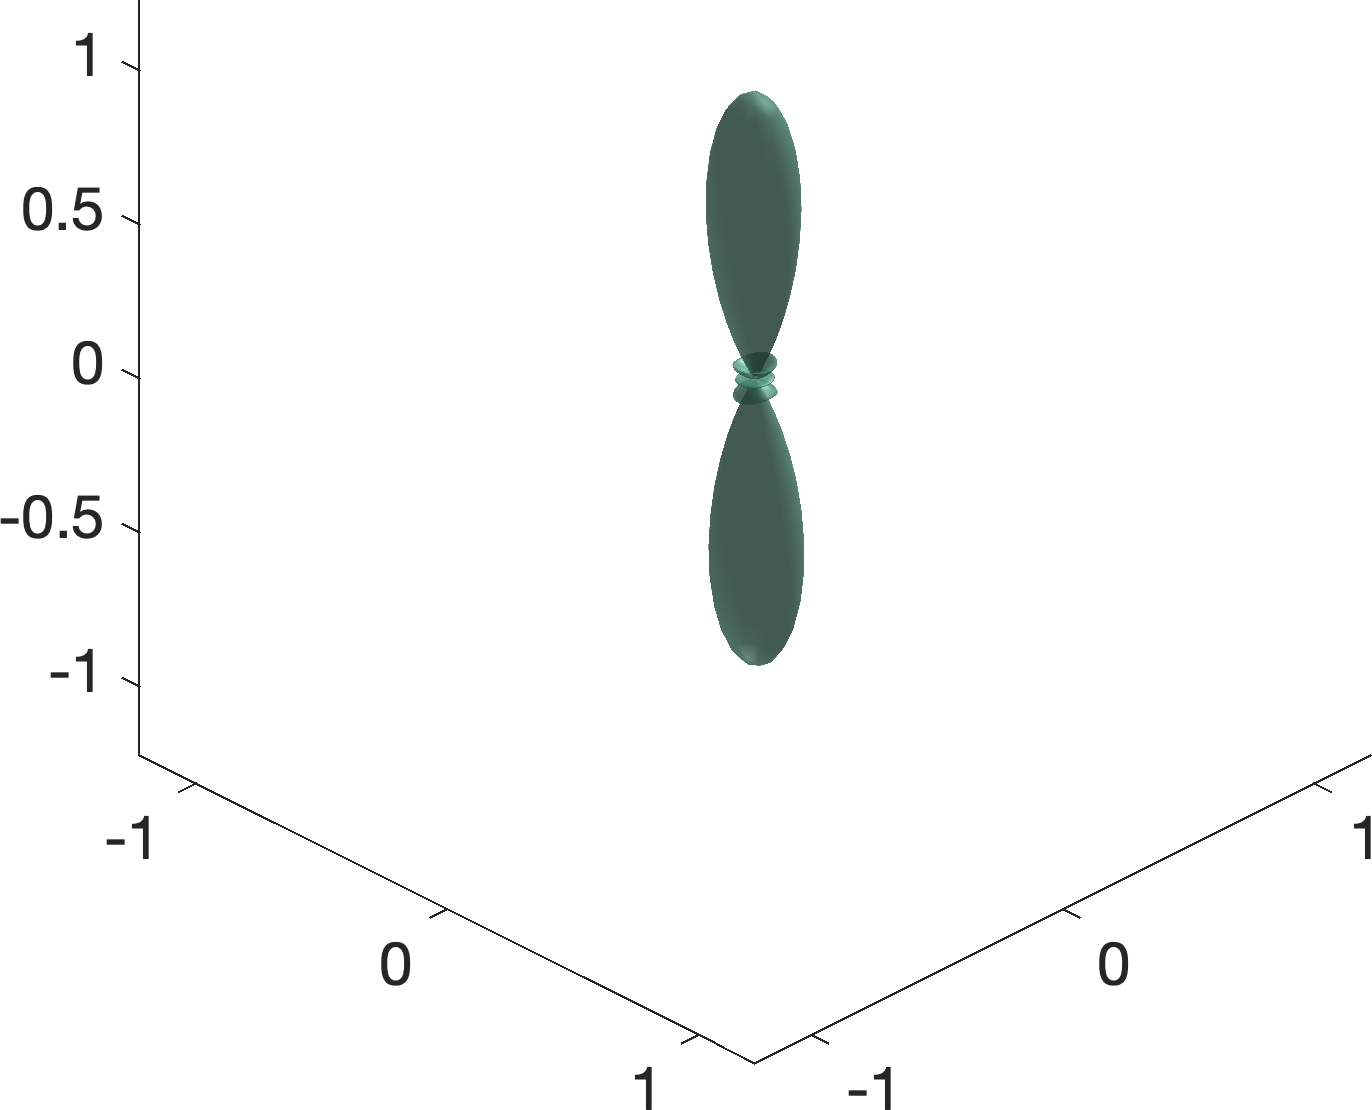
\includegraphics[width=\textwidth]{figures/frf_experiment/fibres_fod_3D_kappa100_b_3000n_1}
  \end{subfigure}
  \begin{subfigure}[]{0.245\textwidth}
    \caption*{10th percentile}
    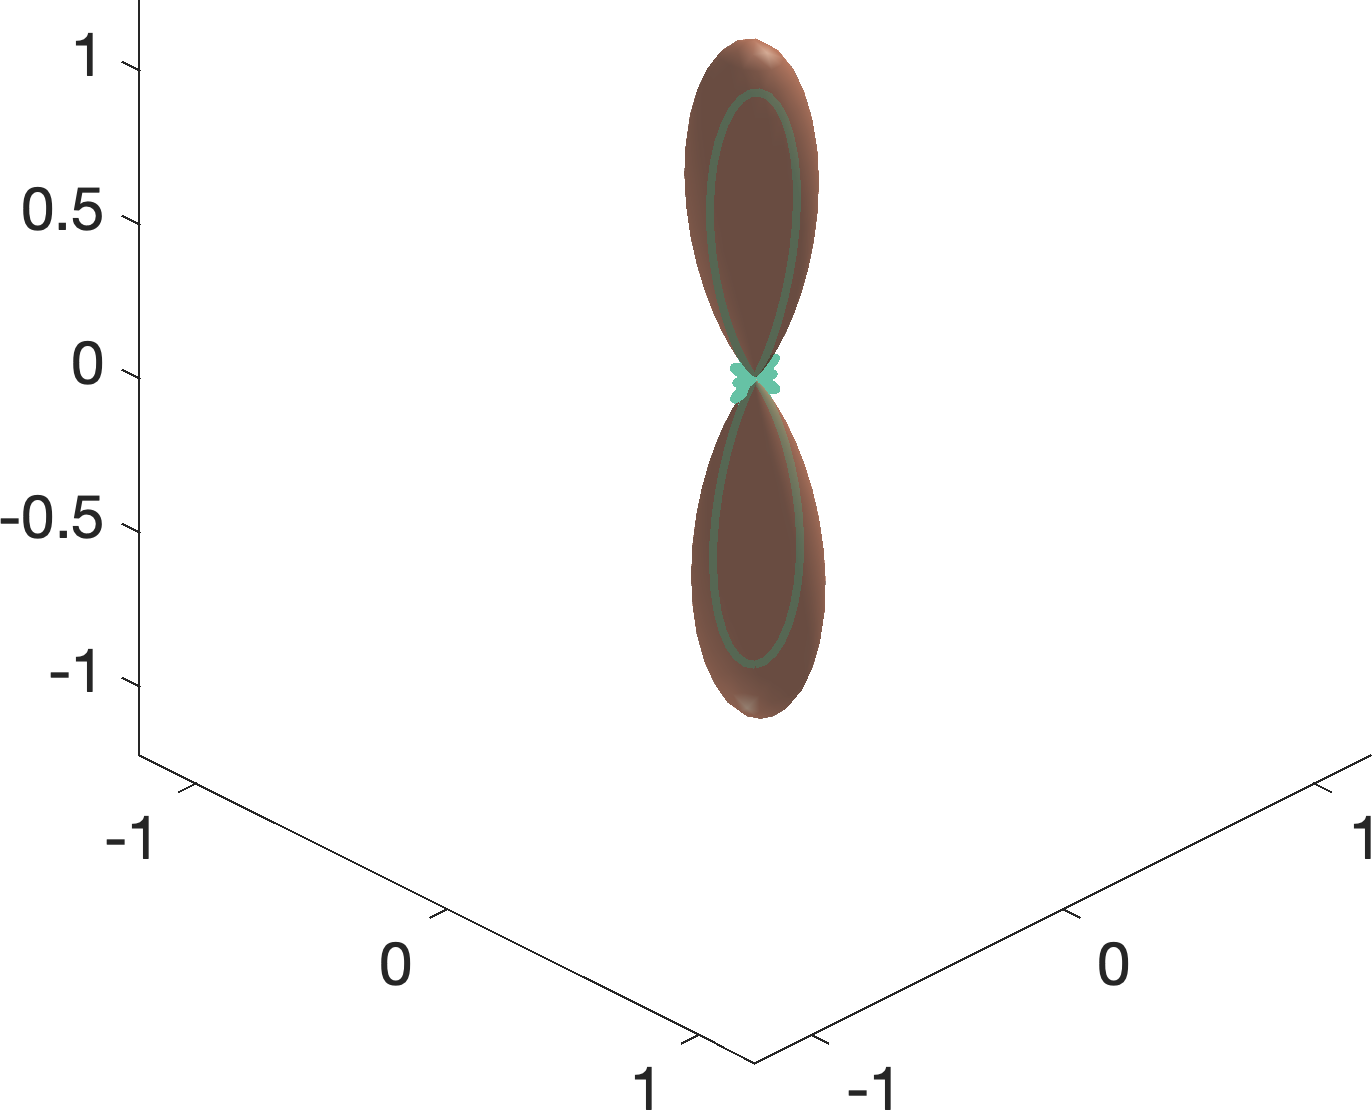
\includegraphics[width=\textwidth]{figures/frf_experiment/fibres_fod_3D_kappa100_b_3000n_2}
  \end{subfigure}
  \begin{subfigure}[]{0.245\textwidth}
    \caption*{Median}
    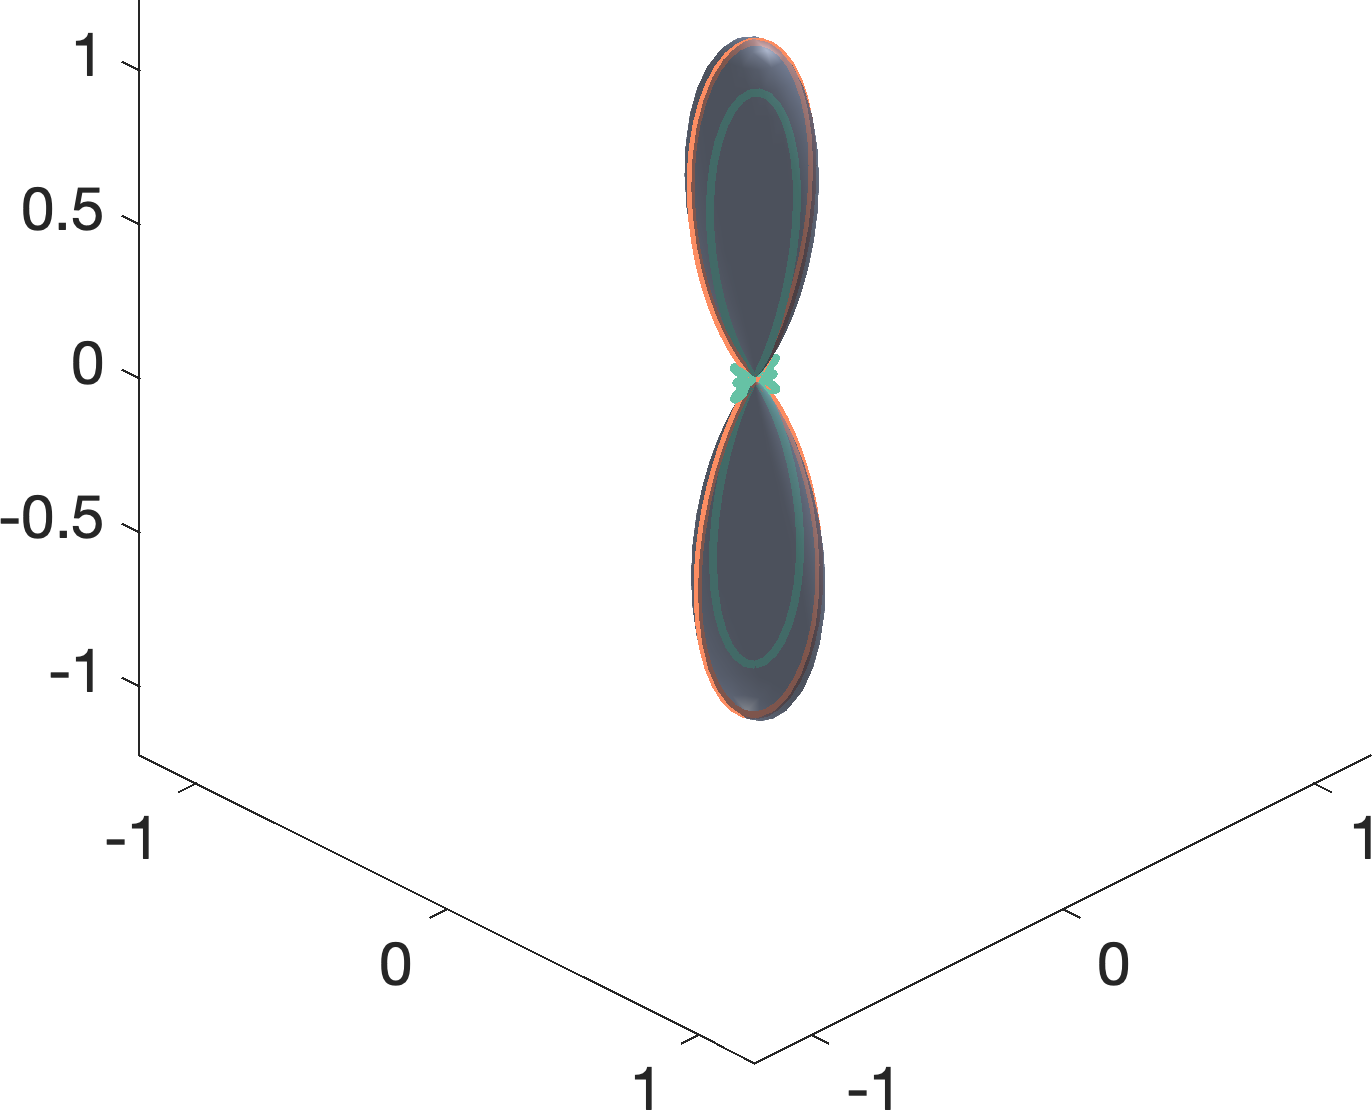
\includegraphics[width=\textwidth]{figures/frf_experiment/fibres_fod_3D_kappa100_b_3000n_3}
  \end{subfigure}
  \begin{subfigure}[]{0.245\textwidth}
    \caption*{90th percentile}
    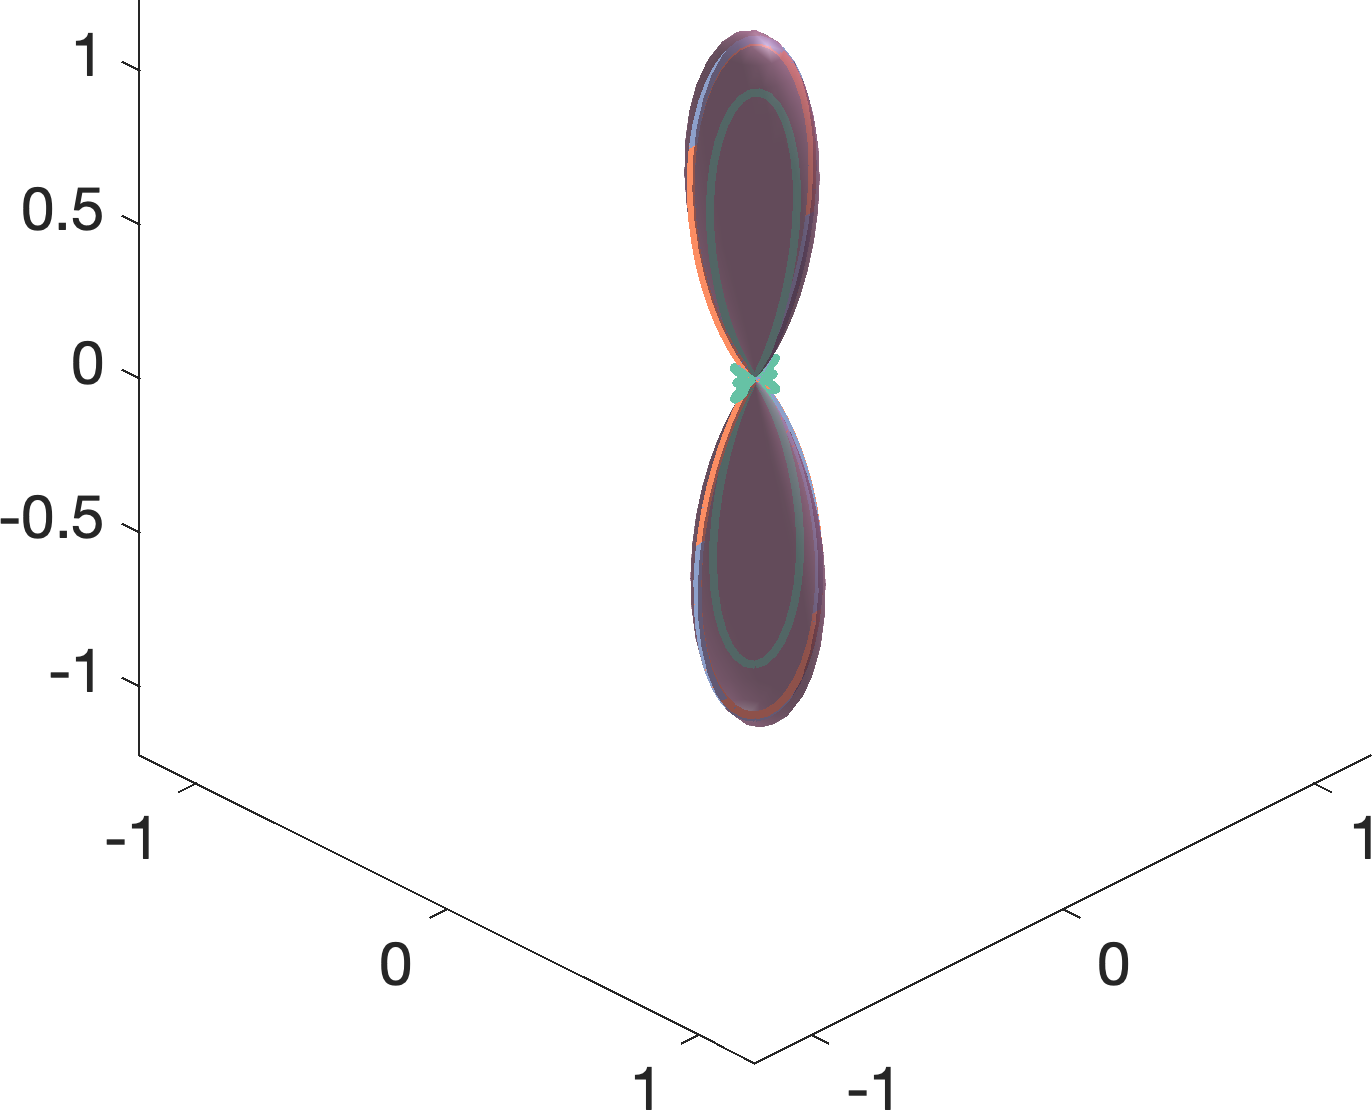
\includegraphics[width=\textwidth]{figures/frf_experiment/fibres_fod_3D_kappa100_b_3000n_4_f1}
  \end{subfigure}
  % \caption{$\kappa = 100$}
  % \end{subfigure}
  \end{minipage}
}

 % \begin{subfigure}[]{\textwidth}
\makebox[\textwidth][c]{
  \begin{minipage}[c]{0.15\textwidth}
    \subcaption{$\kappa = 6$}
  \end{minipage}
  \hfill
  \begin{minipage}[c]{\textwidth}
    \begin{subfigure}[]{0.245\textwidth}
    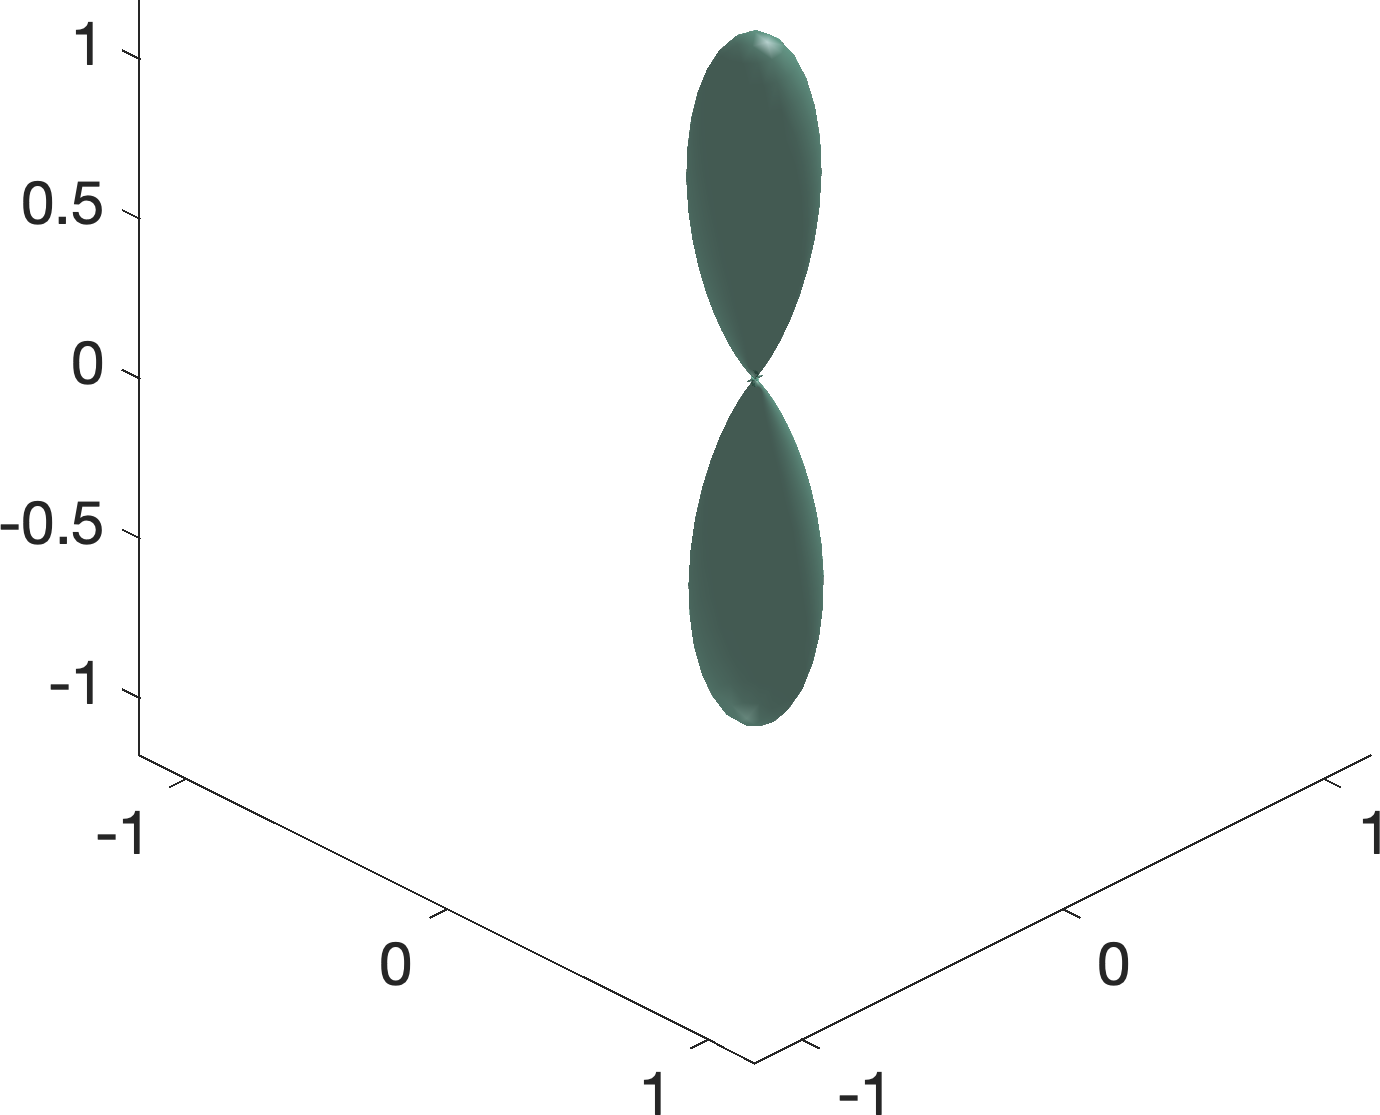
\includegraphics[width=\textwidth]{figures/frf_experiment/fibres_fod_3D_kappa6_b_3000n_1}
  \end{subfigure}
  \begin{subfigure}[]{0.245\textwidth}
    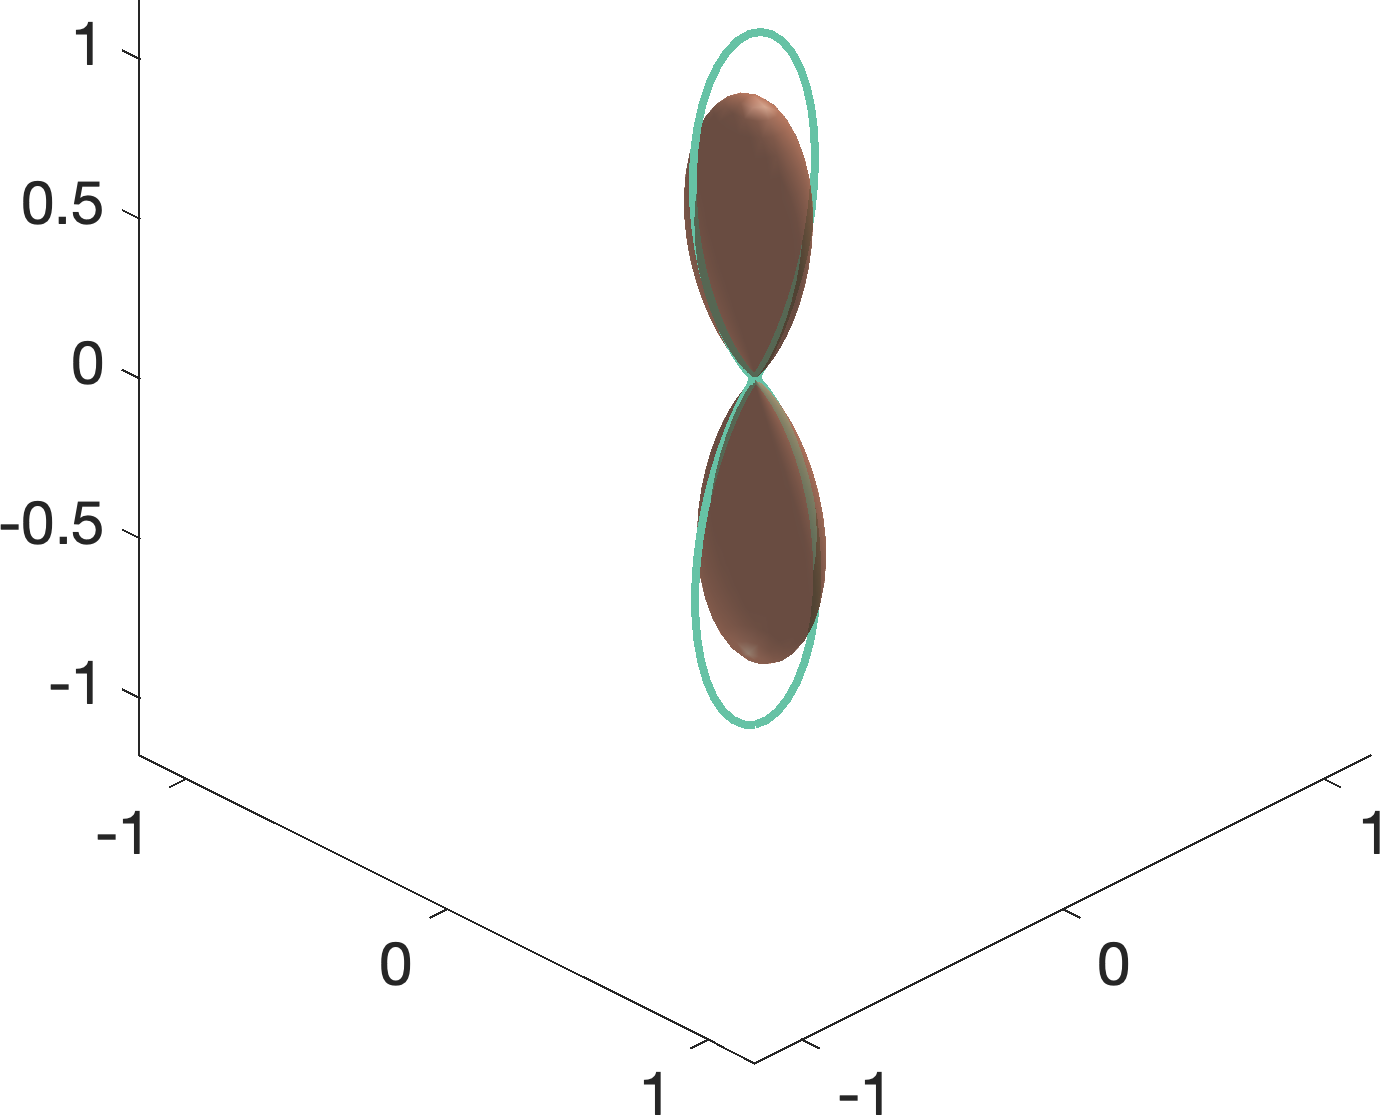
\includegraphics[width=\textwidth]{figures/frf_experiment/fibres_fod_3D_kappa6_b_3000n_2}
  \end{subfigure}
  \begin{subfigure}[]{0.245\textwidth}
    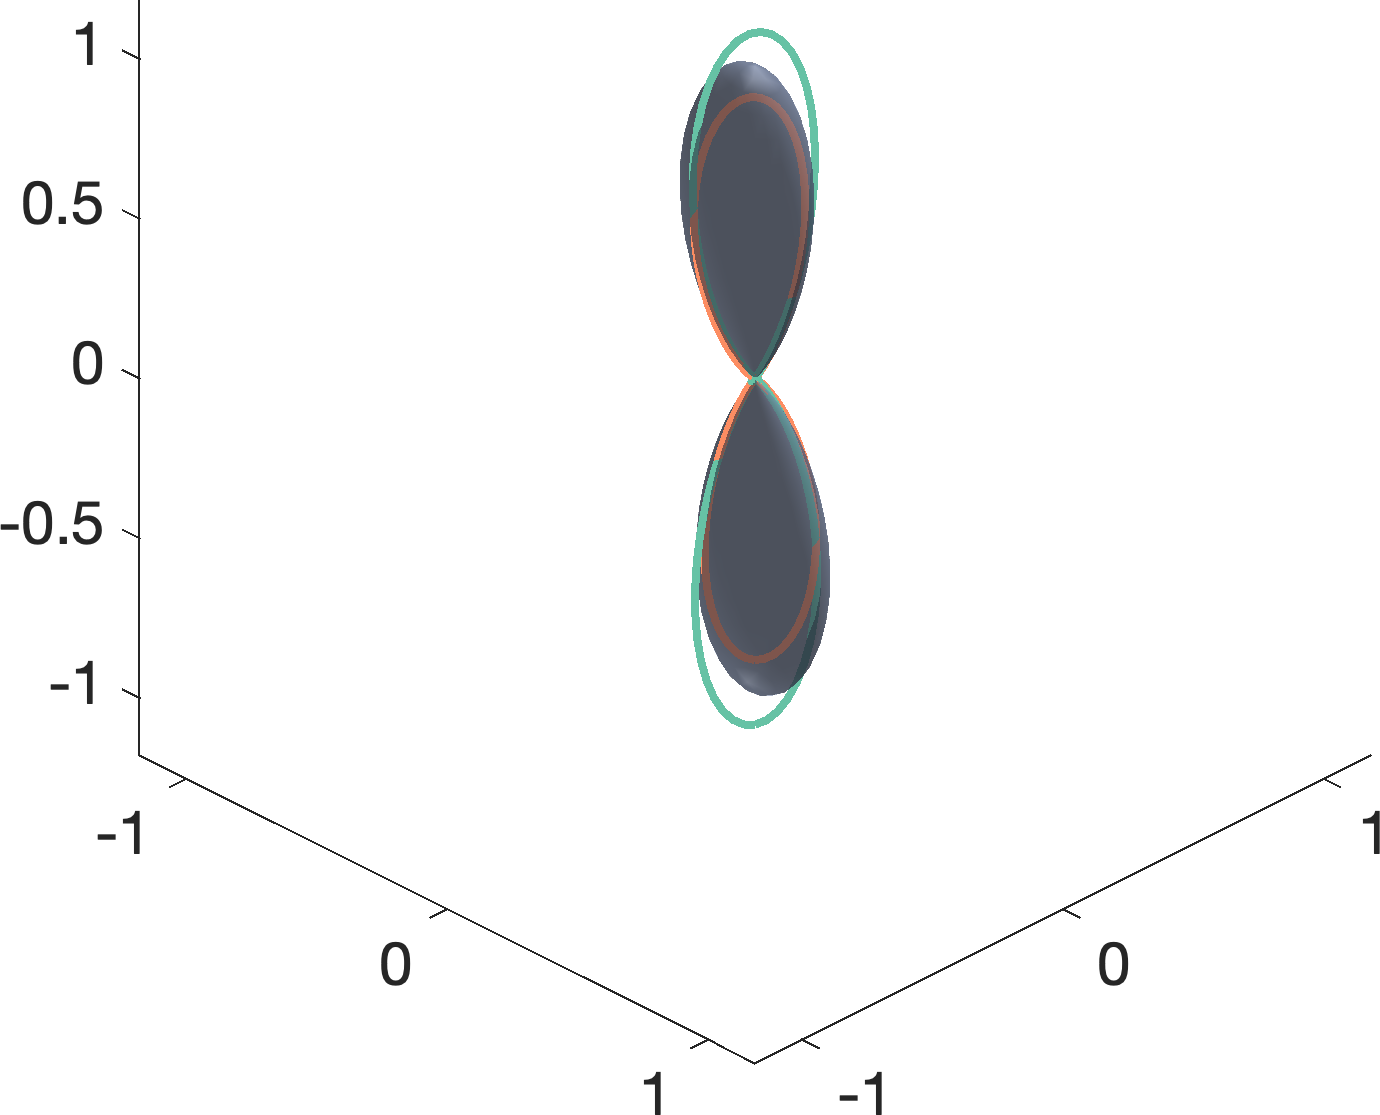
\includegraphics[width=\textwidth]{figures/frf_experiment/fibres_fod_3D_kappa6_b_3000n_3}
  \end{subfigure}
  \begin{subfigure}[]{0.245\textwidth}
    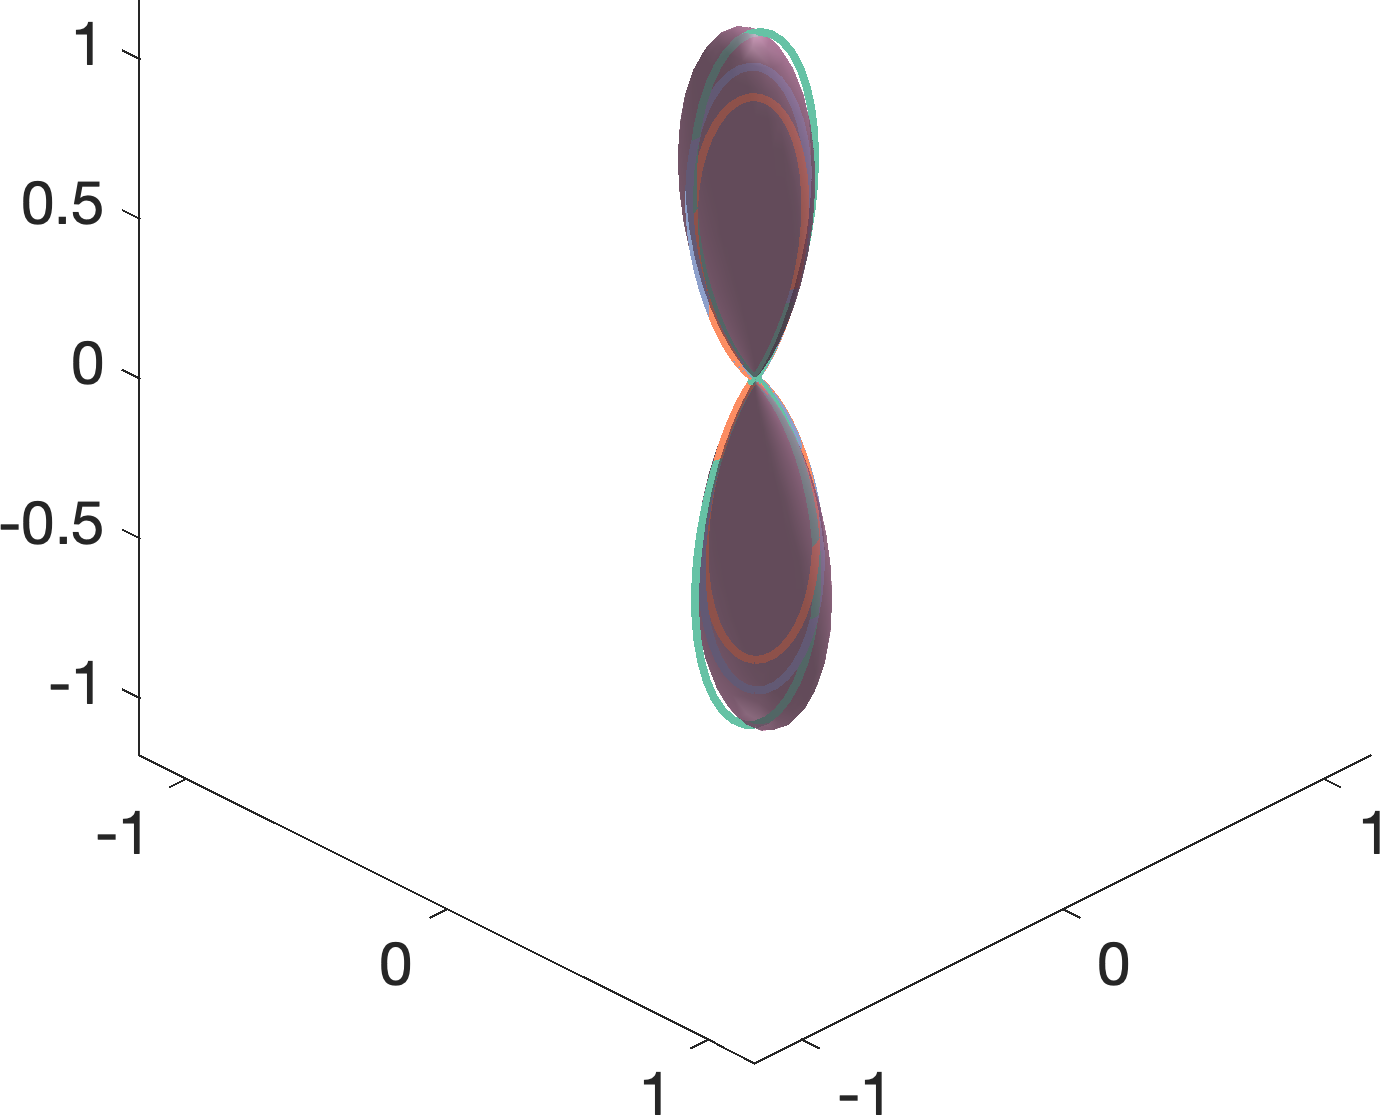
\includegraphics[width=\textwidth]{figures/frf_experiment/fibres_fod_3D_kappa6_b_3000n_4_f1}
  \end{subfigure}
  % \caption{$\kappa = 6$}
  % \end{subfigure}
  \end{minipage}
}
\makebox[\textwidth][c]{
  \begin{minipage}[c]{0.15\textwidth}
    \subcaption{$\kappa = 2$}
  \end{minipage}
  \hfill
  % \begin{subfigure}[]{\textwidth}
  \begin{minipage}[c]{\textwidth}
    \begin{subfigure}[]{0.245\textwidth}
    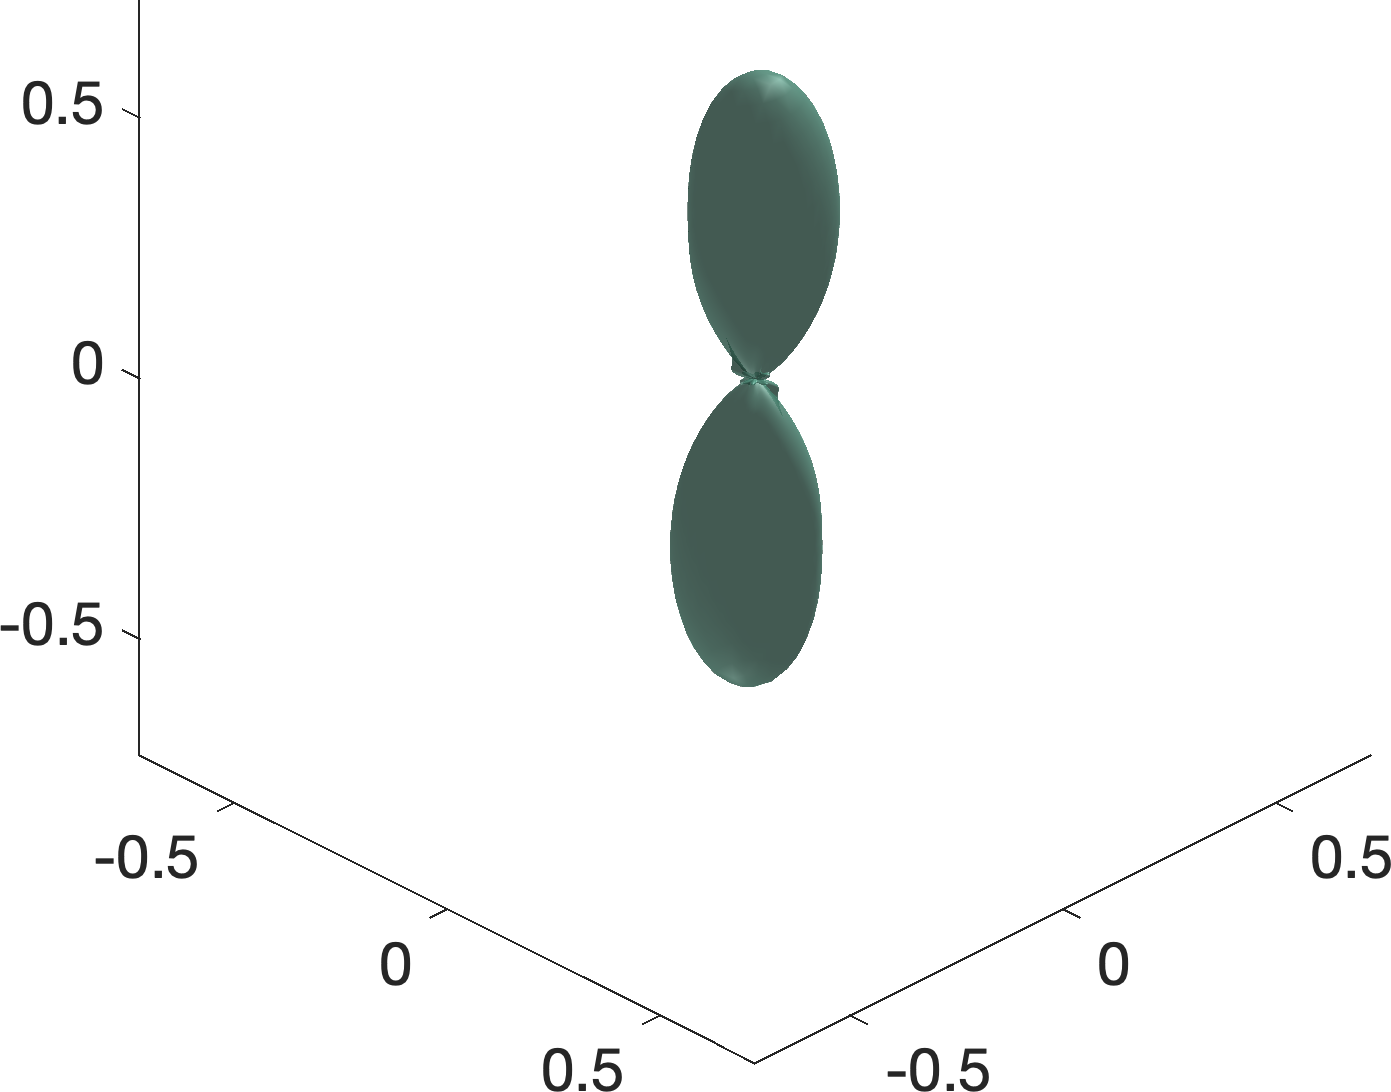
\includegraphics[width=\textwidth]{figures/frf_experiment/fibres_fod_3D_kappa2_b_3000n_1}
  \end{subfigure}
  \begin{subfigure}[]{0.245\textwidth}
    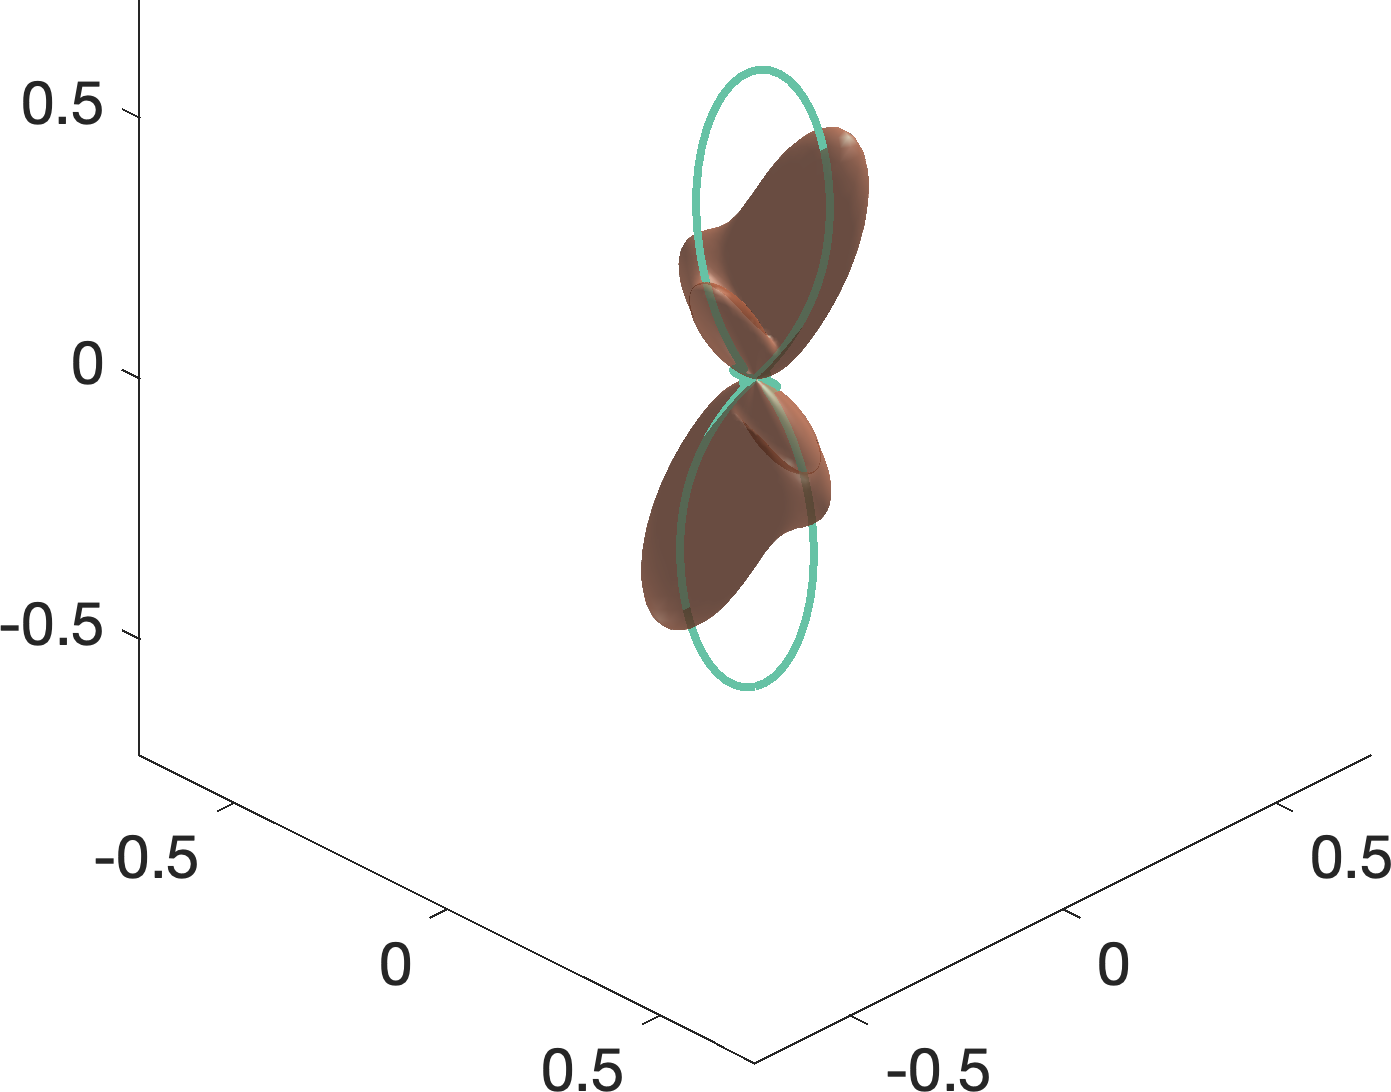
\includegraphics[width=\textwidth]{figures/frf_experiment/fibres_fod_3D_kappa2_b_3000n_2}
  \end{subfigure}
  \begin{subfigure}[]{0.245\textwidth}
    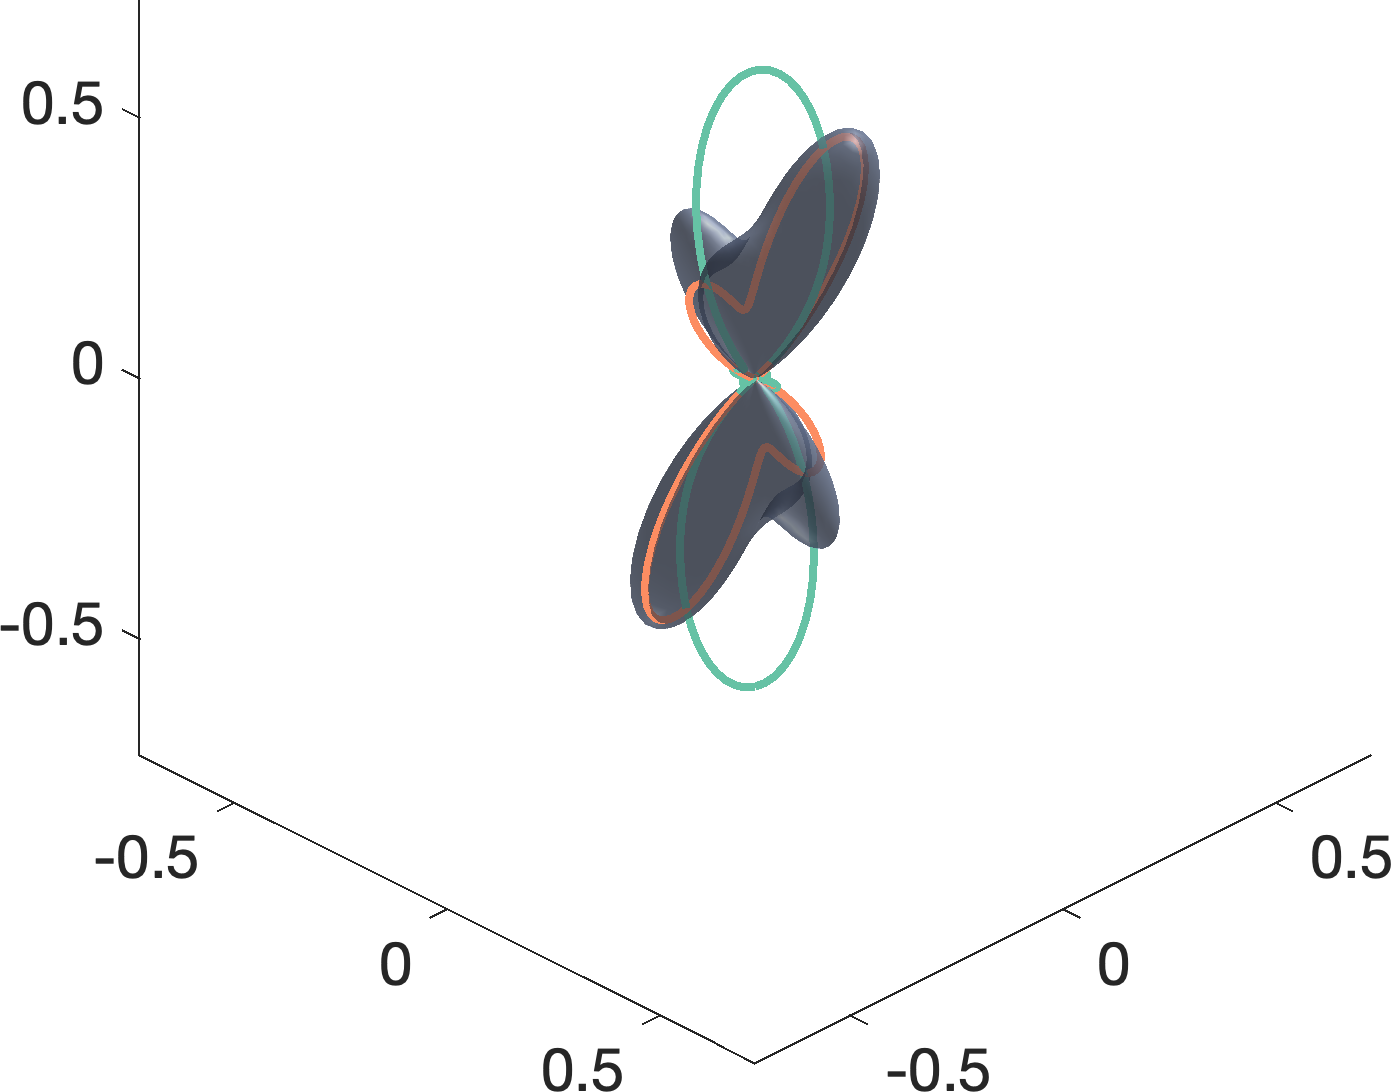
\includegraphics[width=\textwidth]{figures/frf_experiment/fibres_fod_3D_kappa2_b_3000n_3}
  \end{subfigure}
  \begin{subfigure}[]{0.245\textwidth}
    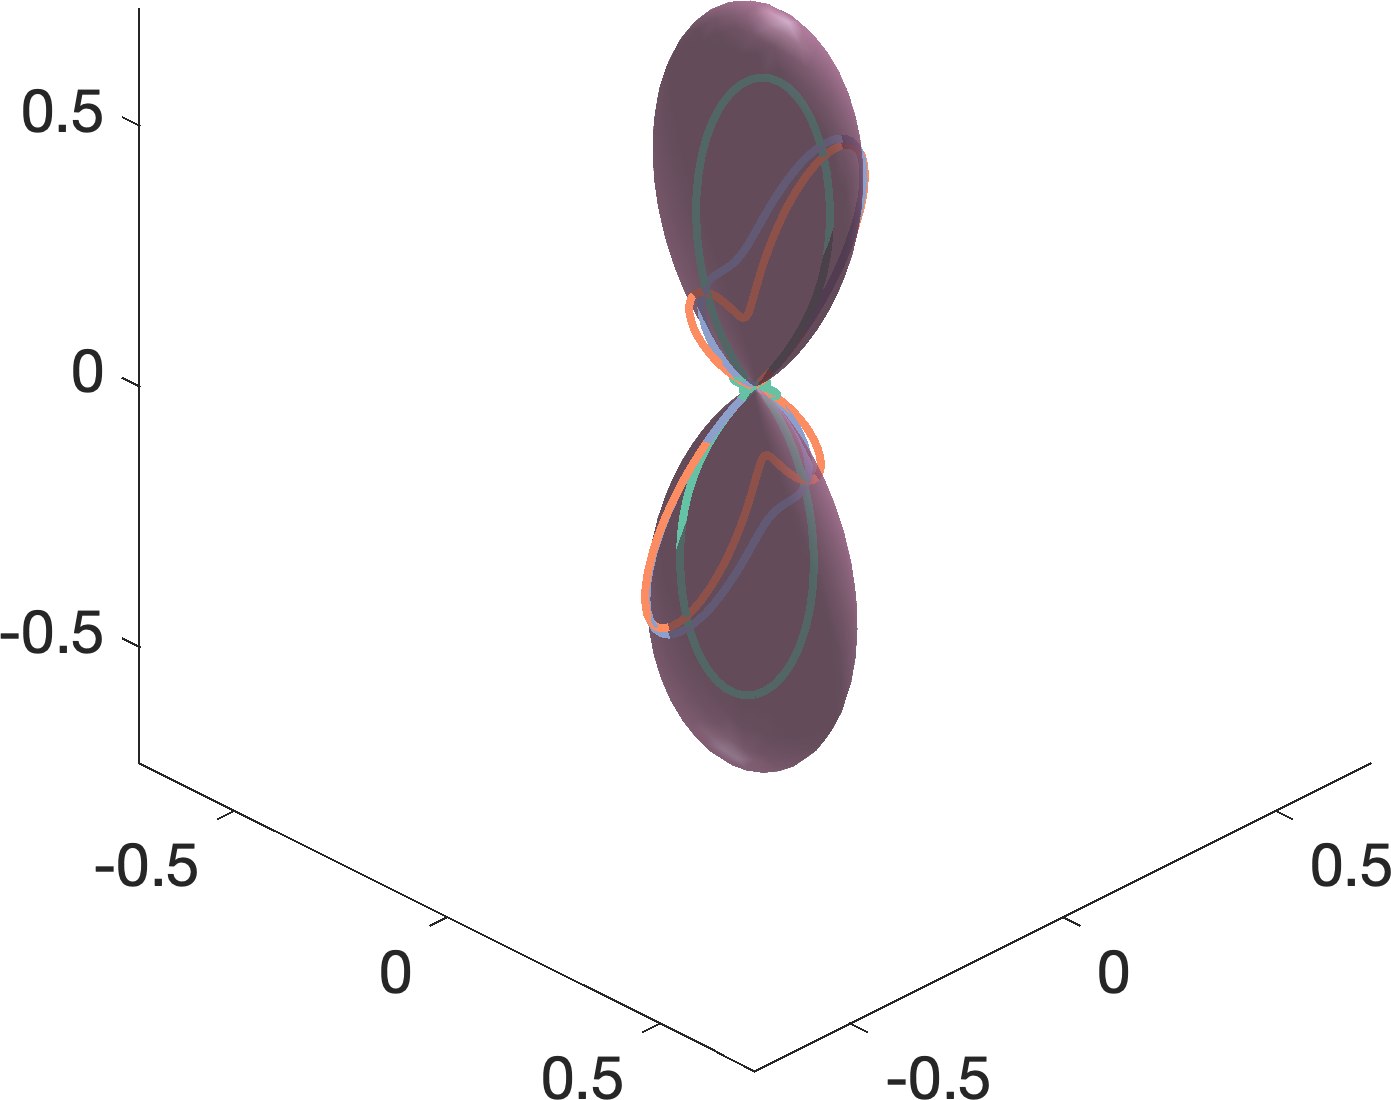
\includegraphics[width=\textwidth]{figures/frf_experiment/fibres_fod_3D_kappa2_b_3000n_4_f1}
  \end{subfigure}
  % \caption{$\kappa = 2$}
  % \end{subfigure}
  \end{minipage}
}
\makebox[\textwidth][c]{
  \begin{minipage}[c]{0.15\textwidth}
    \subcaption{Two crossing}
  \end{minipage}
  \hfill
  \begin{minipage}[c]{\textwidth}
  % \begin{subfigure}[]{\textwidth}
    \begin{subfigure}[]{0.245\textwidth}
    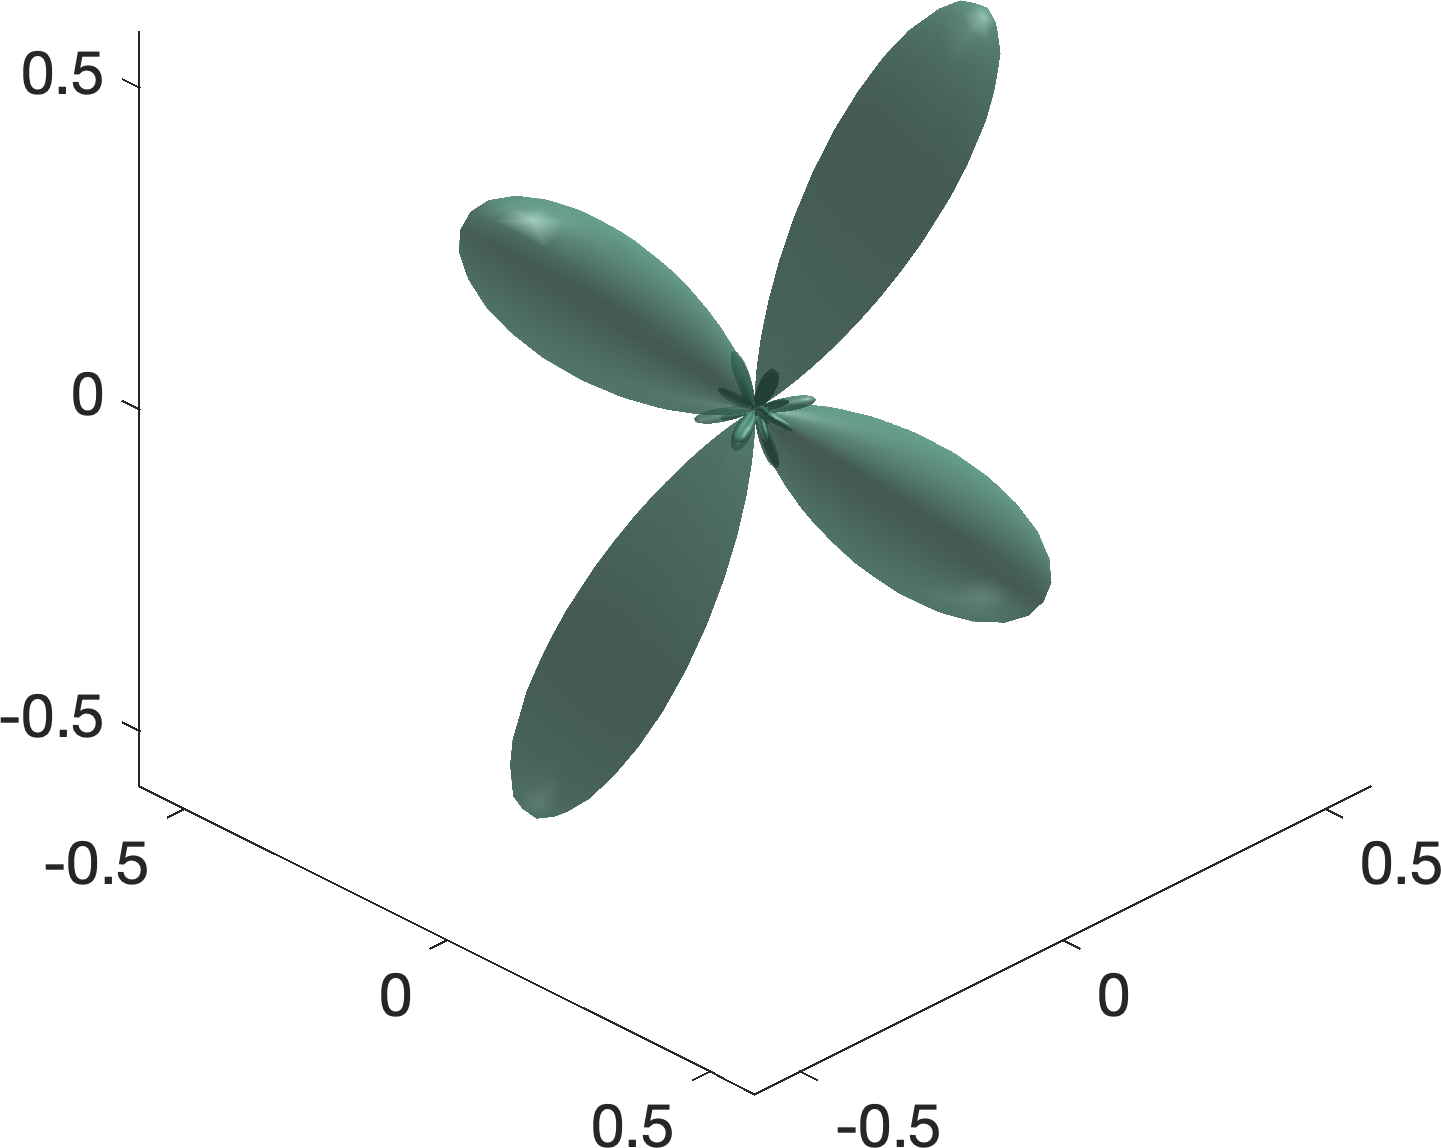
\includegraphics[width=\textwidth]{figures/frf_experiment/twoperp_fod_3D_b_3000n_1}
  \end{subfigure}
  \begin{subfigure}[]{0.245\textwidth}
    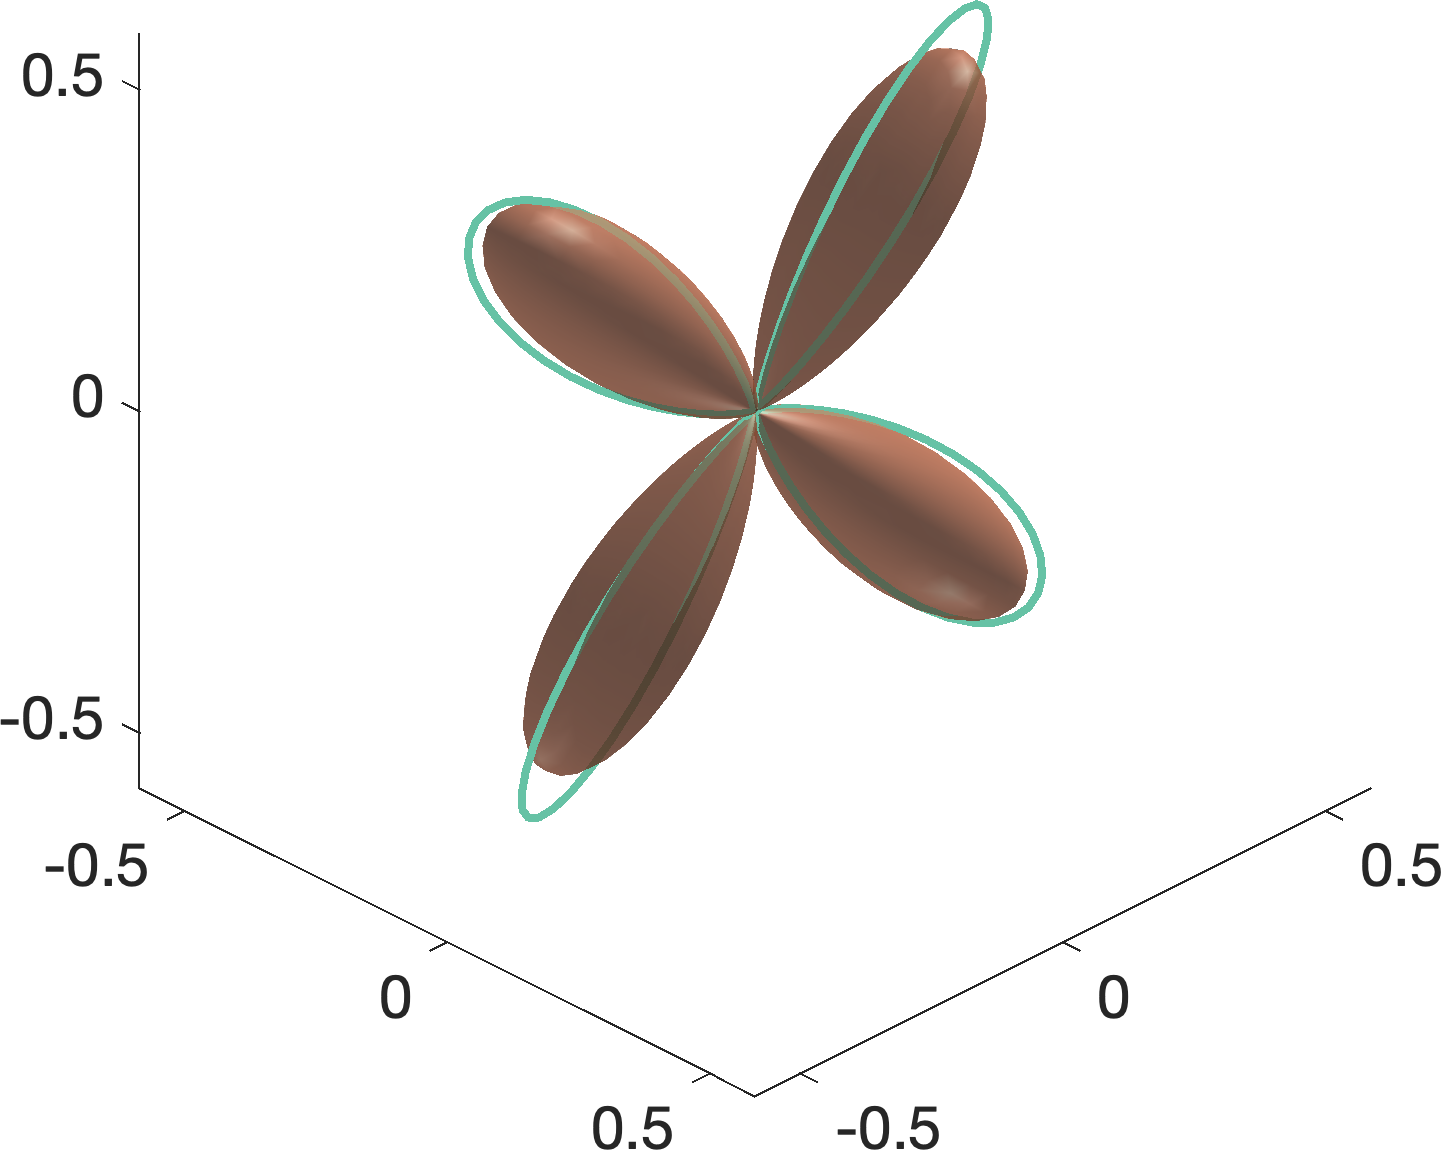
\includegraphics[width=\textwidth]{figures/frf_experiment/twoperp_fod_3D_b_3000n_2}
  \end{subfigure}
  \begin{subfigure}[]{0.245\textwidth}
    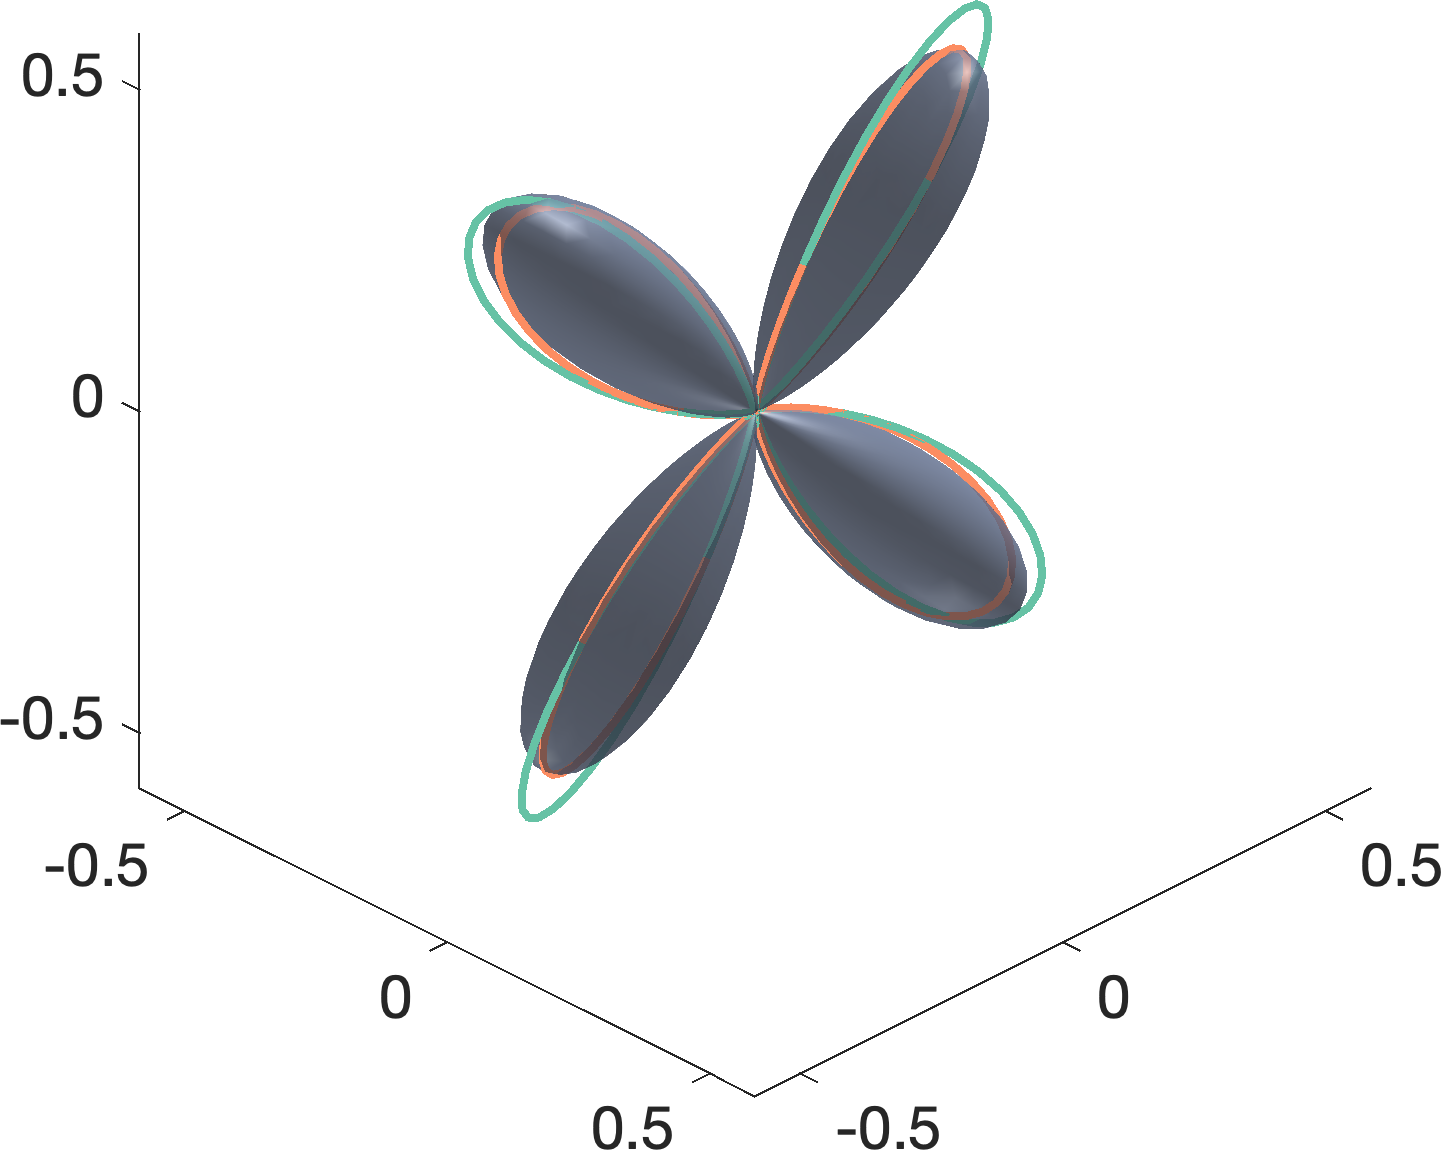
\includegraphics[width=\textwidth]{figures/frf_experiment/twoperp_fod_3D_b_3000n_3}
  \end{subfigure}
  \begin{subfigure}[]{0.245\textwidth}
    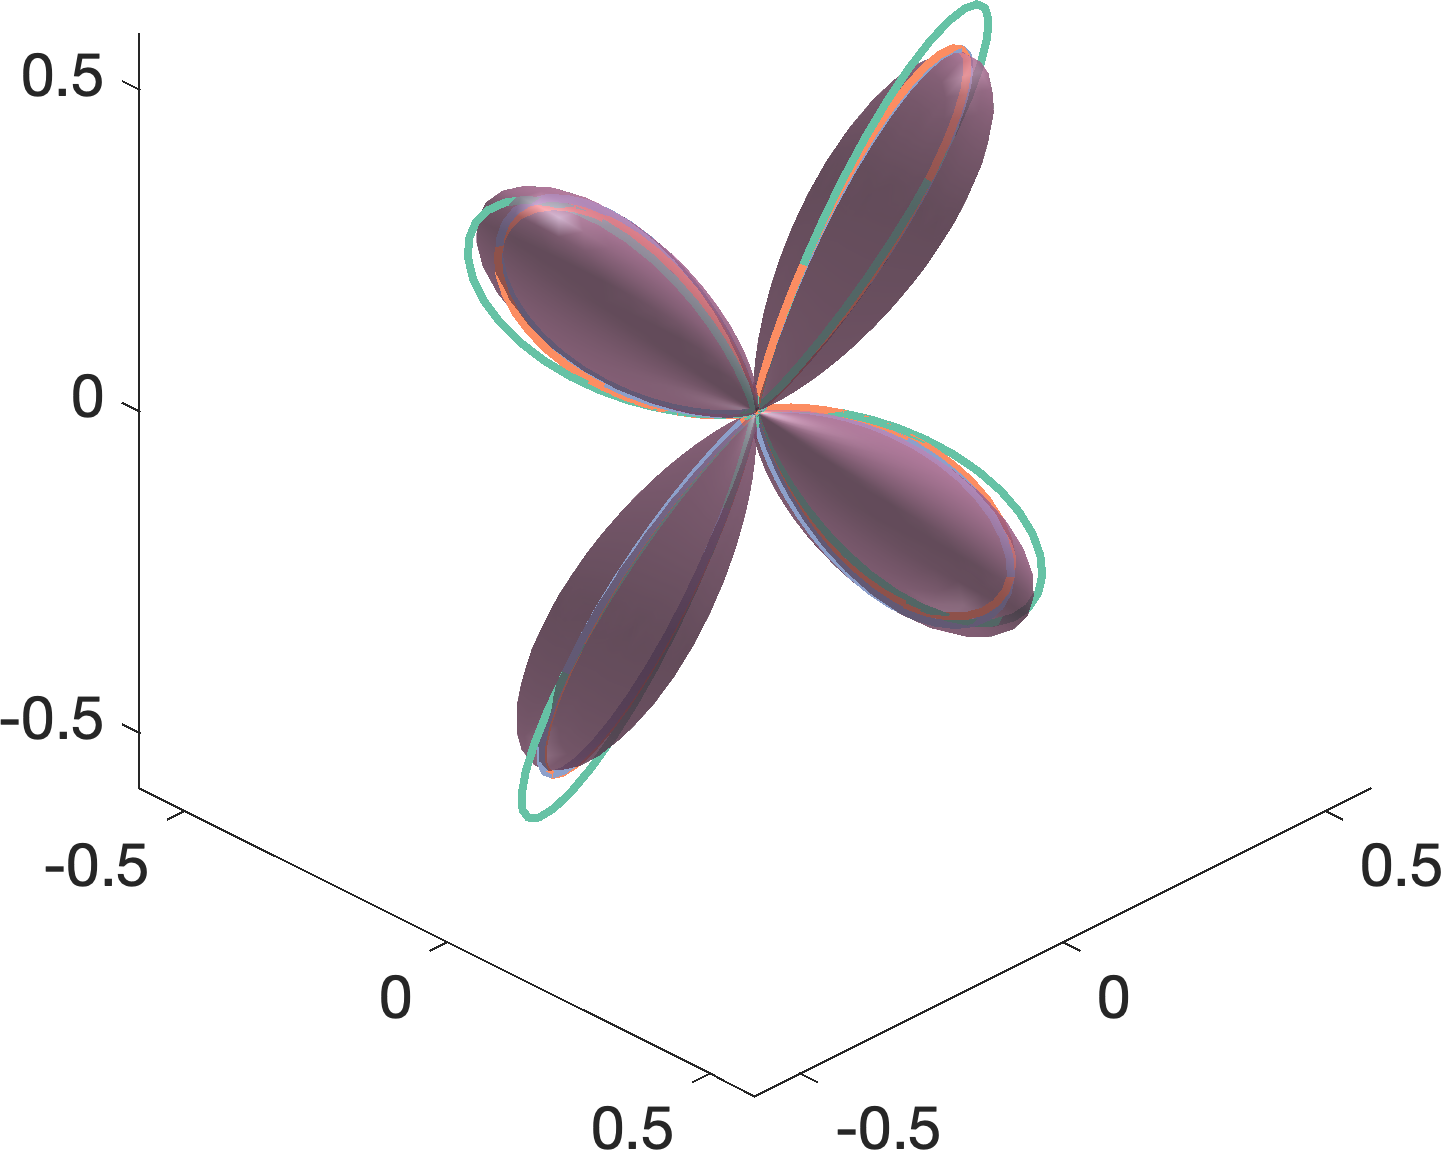
\includegraphics[width=\textwidth]{figures/frf_experiment/twoperp_fod_3D_b_3000n_4_f1}
  \end{subfigure}
  % \caption{Two crossing}
  % \end{subfigure}
  \end{minipage}
}
\makebox[\textwidth][c]{
  \begin{minipage}[c]{0.15\textwidth}
    \subcaption{Three crossing}
  \end{minipage}
  \hfill
  \begin{minipage}[c]{\textwidth}
  % \begin{subfigure}[]{\textwidth}
    \begin{subfigure}[]{0.245\textwidth}
      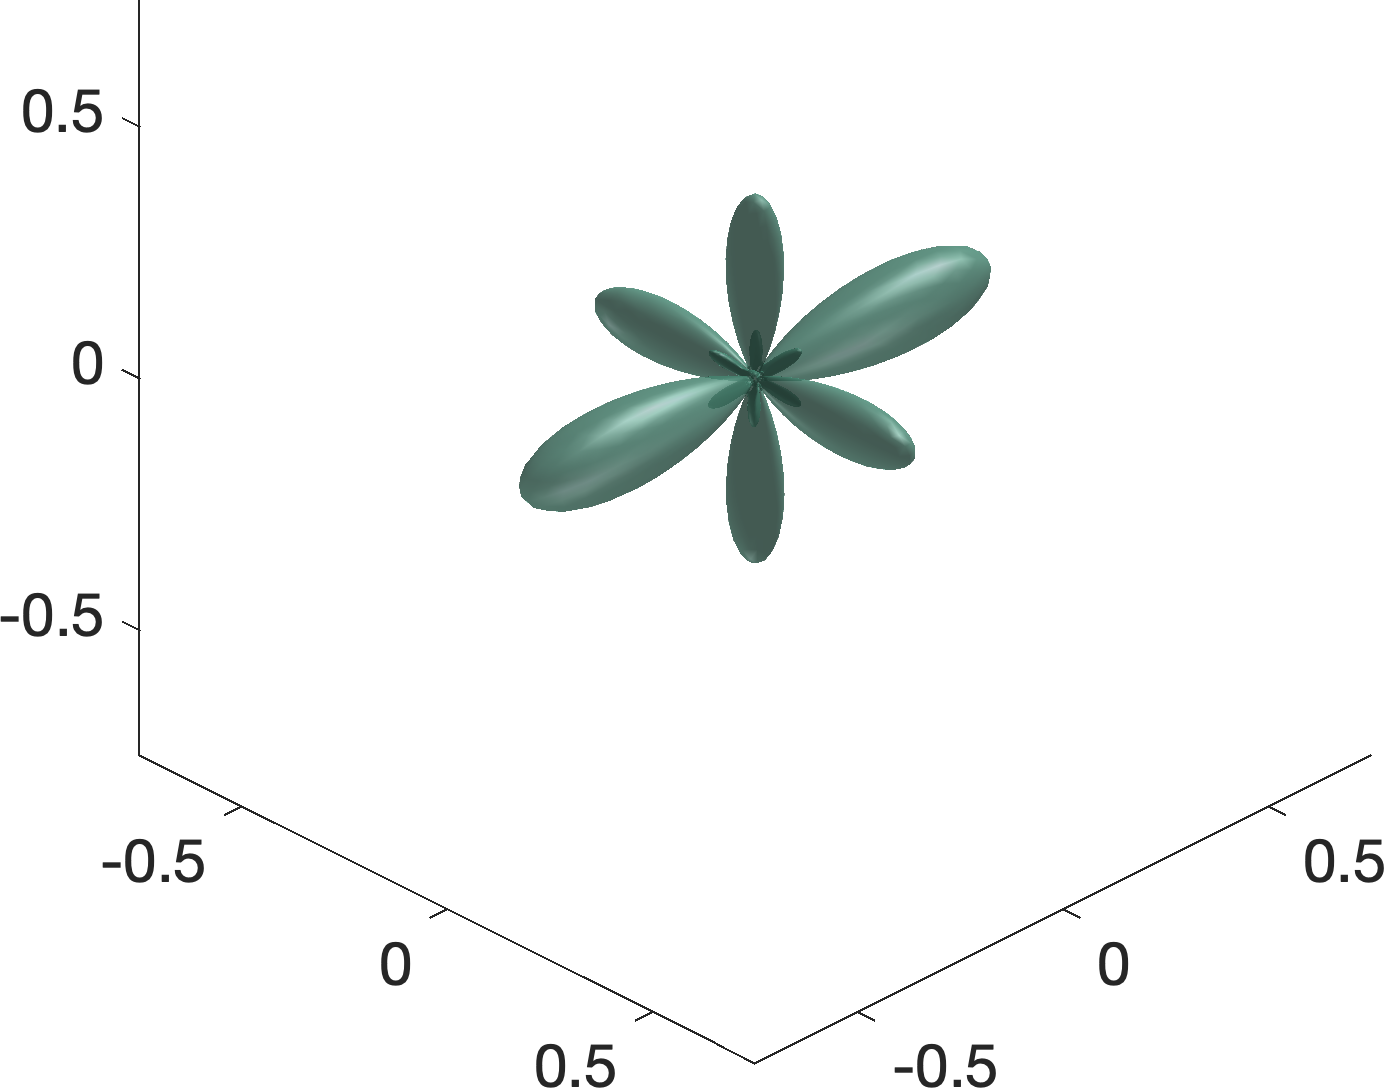
\includegraphics[width=\textwidth]{figures/frf_experiment/threeperp_fod_3D_b_3000n_1}
  \end{subfigure}
  \begin{subfigure}[]{0.245\textwidth}
    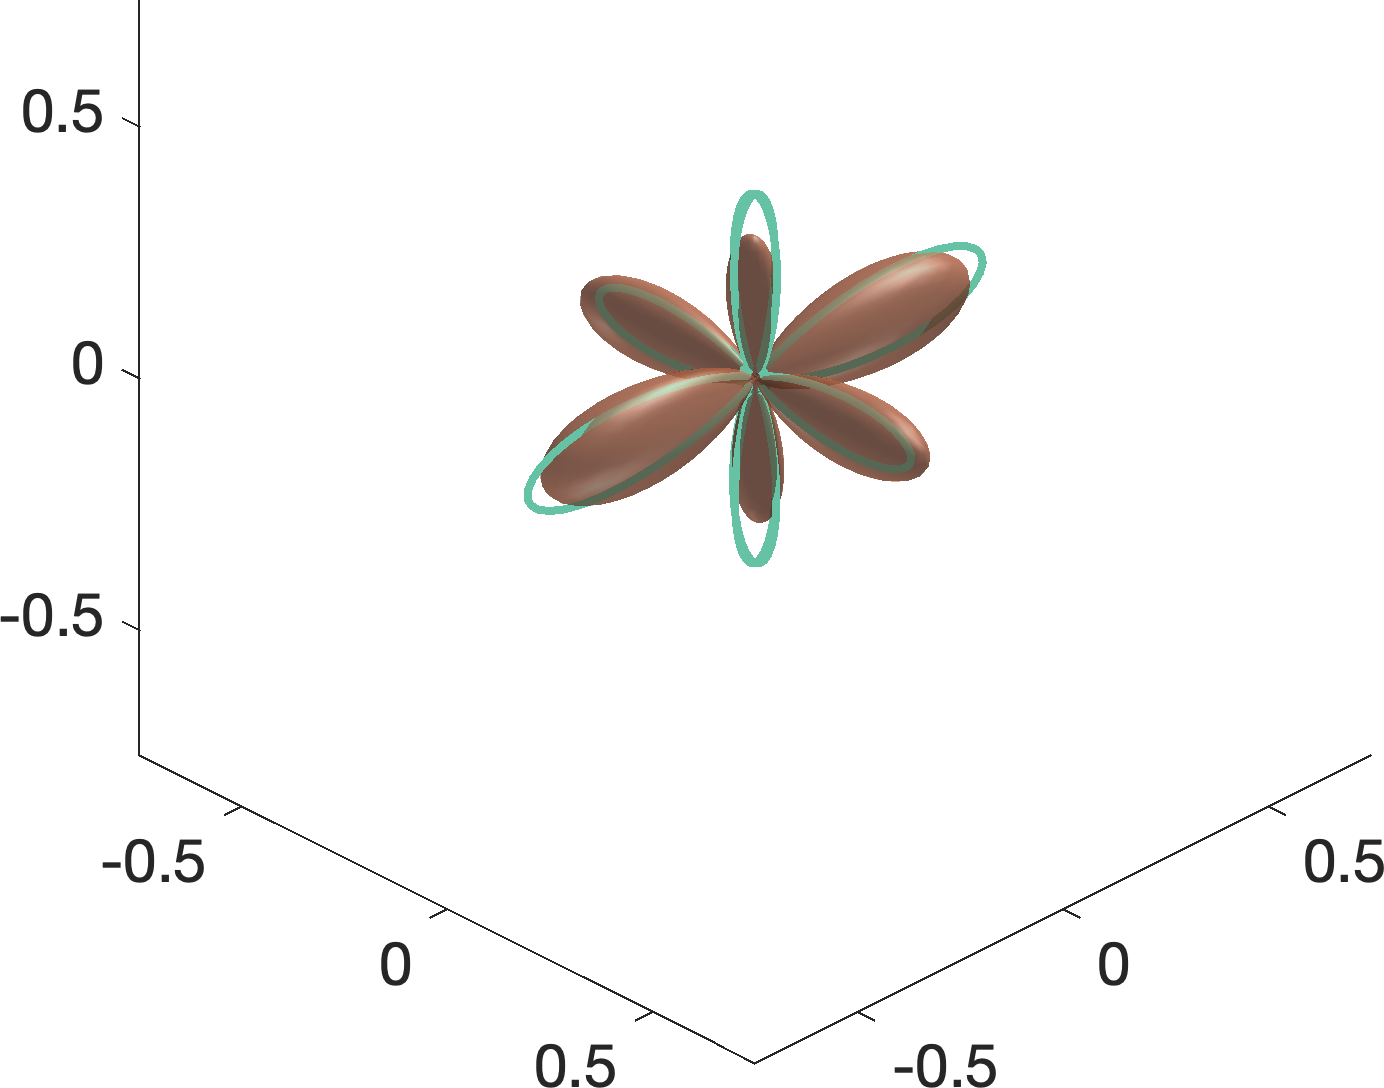
\includegraphics[width=\textwidth]{figures/frf_experiment/threeperp_fod_3D_b_3000n_2}
  \end{subfigure}
  \begin{subfigure}[]{0.245\textwidth}
    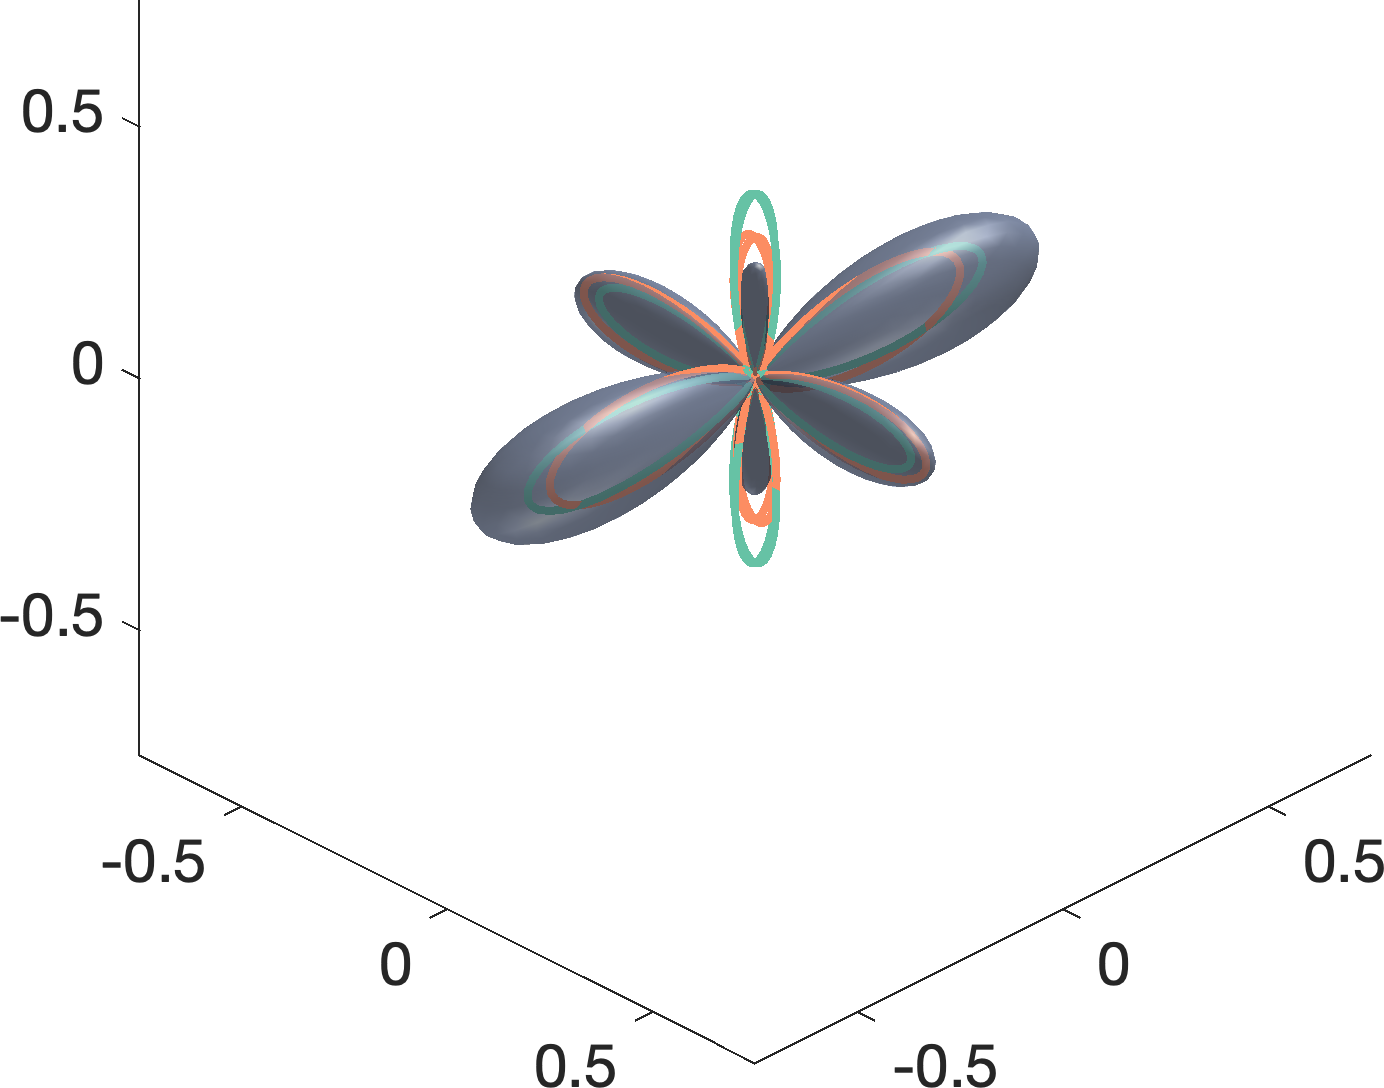
\includegraphics[width=\textwidth]{figures/frf_experiment/threeperp_fod_3D_b_3000n_3}
  \end{subfigure}
  \begin{subfigure}[]{0.245\textwidth}
    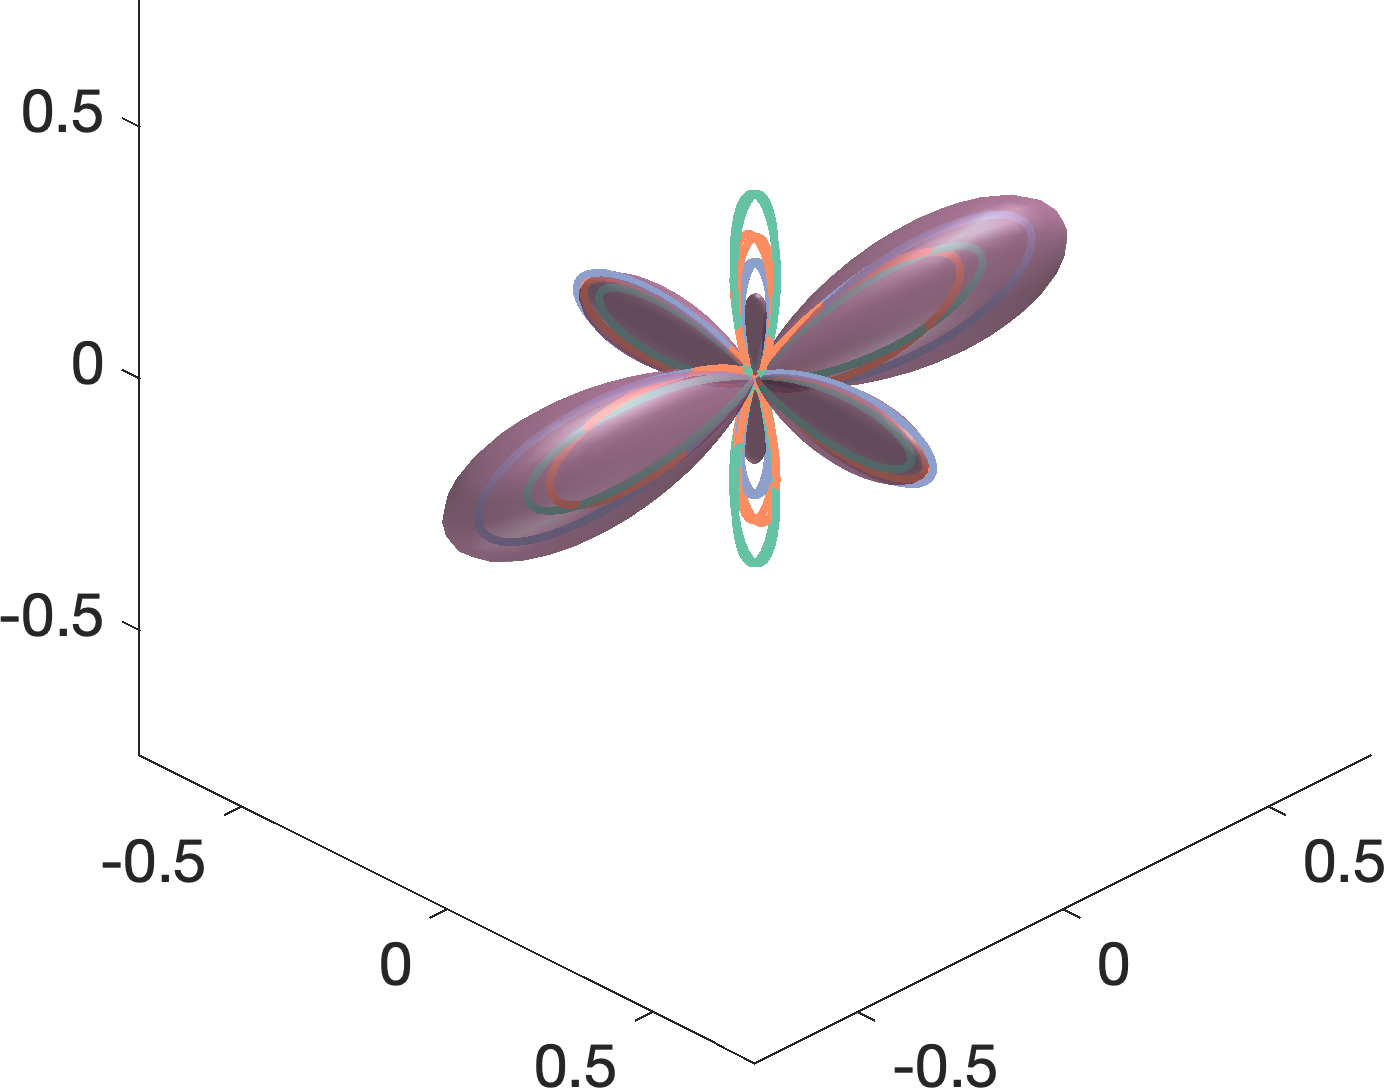
\includegraphics[width=\textwidth]{figures/frf_experiment/threeperp_fod_3D_b_3000n_4_f1}
  \end{subfigure}
  % \caption{Three crossing}
  % \end{subfigure}
  \end{minipage}
}
\makebox[\textwidth][c]{
  \begin{minipage}[c]{0.15\textwidth}
    \subcaption{EM fibres}
  \end{minipage}
  \hfill
  \begin{minipage}[c]{\textwidth}
 % \begin{subfigure}[]{\textwidth}
    \begin{subfigure}[]{0.245\textwidth}
      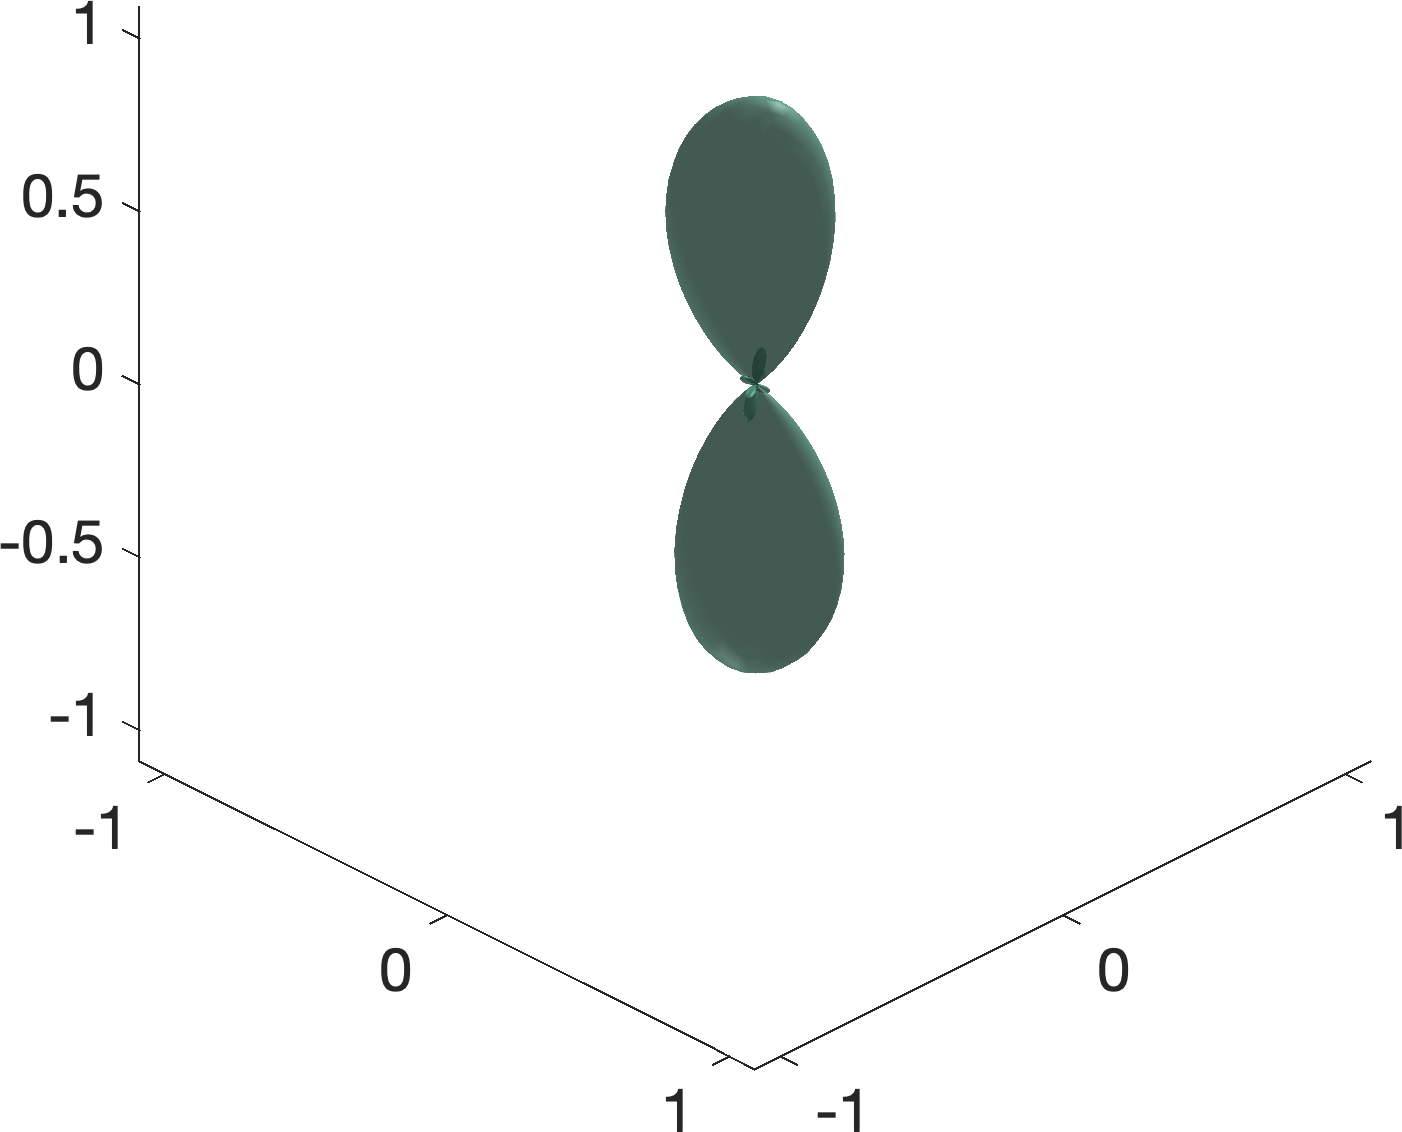
\includegraphics[width=\textwidth]{figures/frf_experiment/EMfibres_fod_3D_b_3000n_1}

  \end{subfigure}
  \begin{subfigure}[]{0.245\textwidth}
    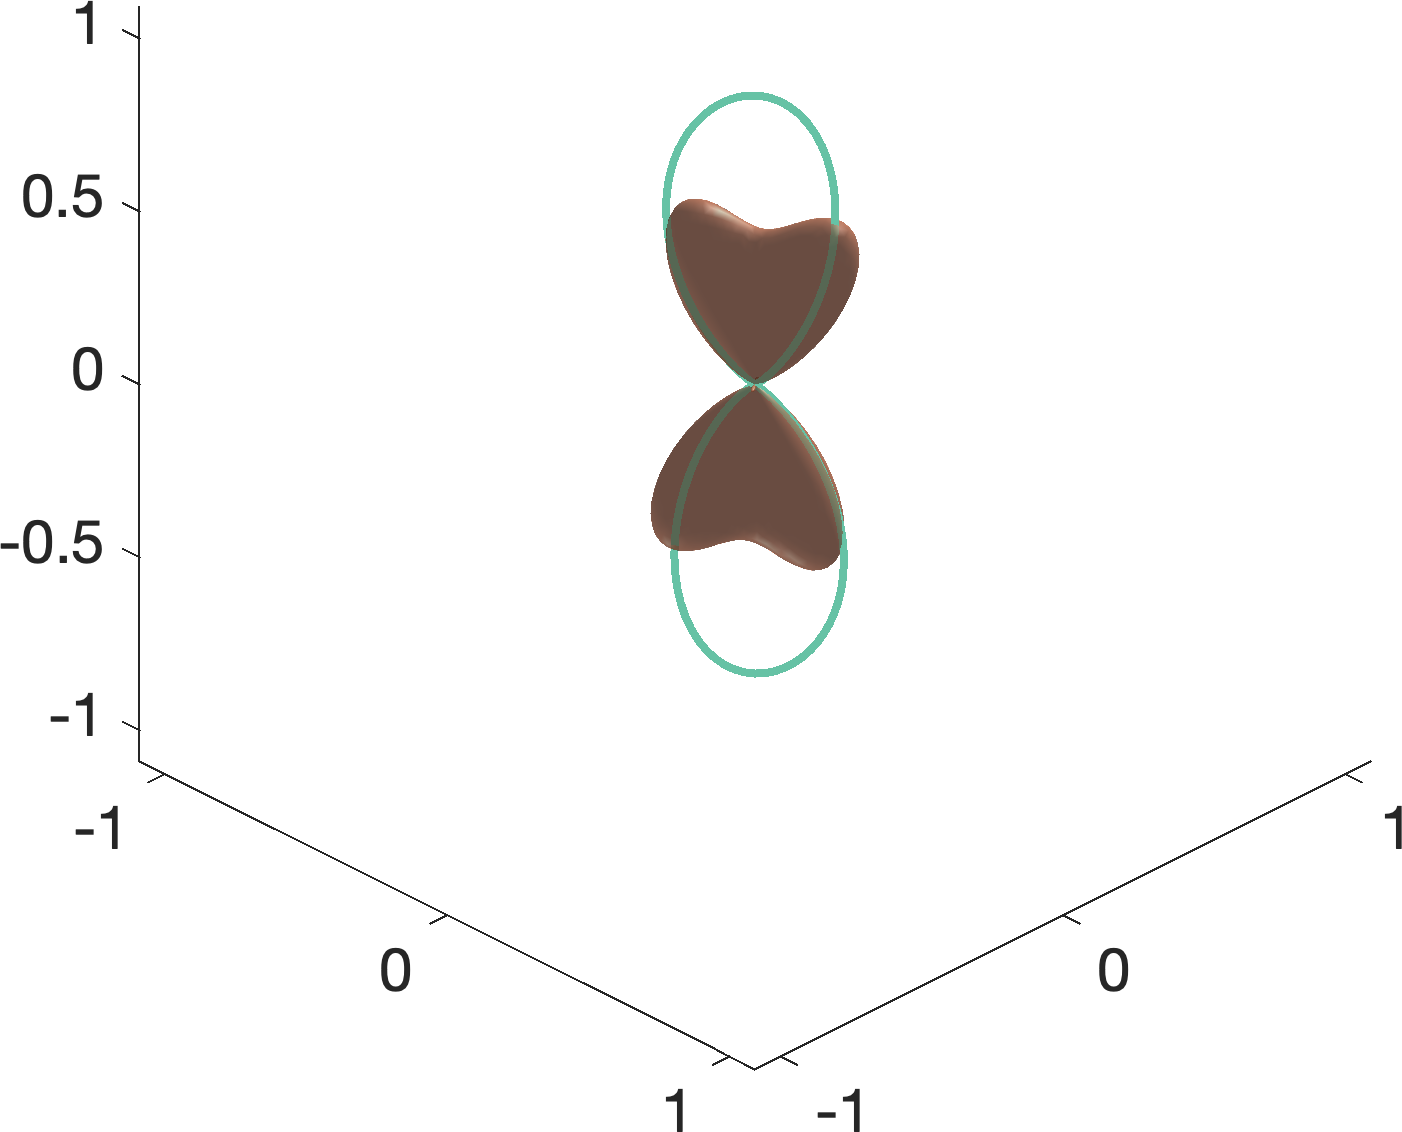
\includegraphics[width=\textwidth]{figures/frf_experiment/EMfibres_fod_3D_b_3000n_2}
    % \caption*{10th percentile}
  \end{subfigure}
  \begin{subfigure}[]{0.245\textwidth}
    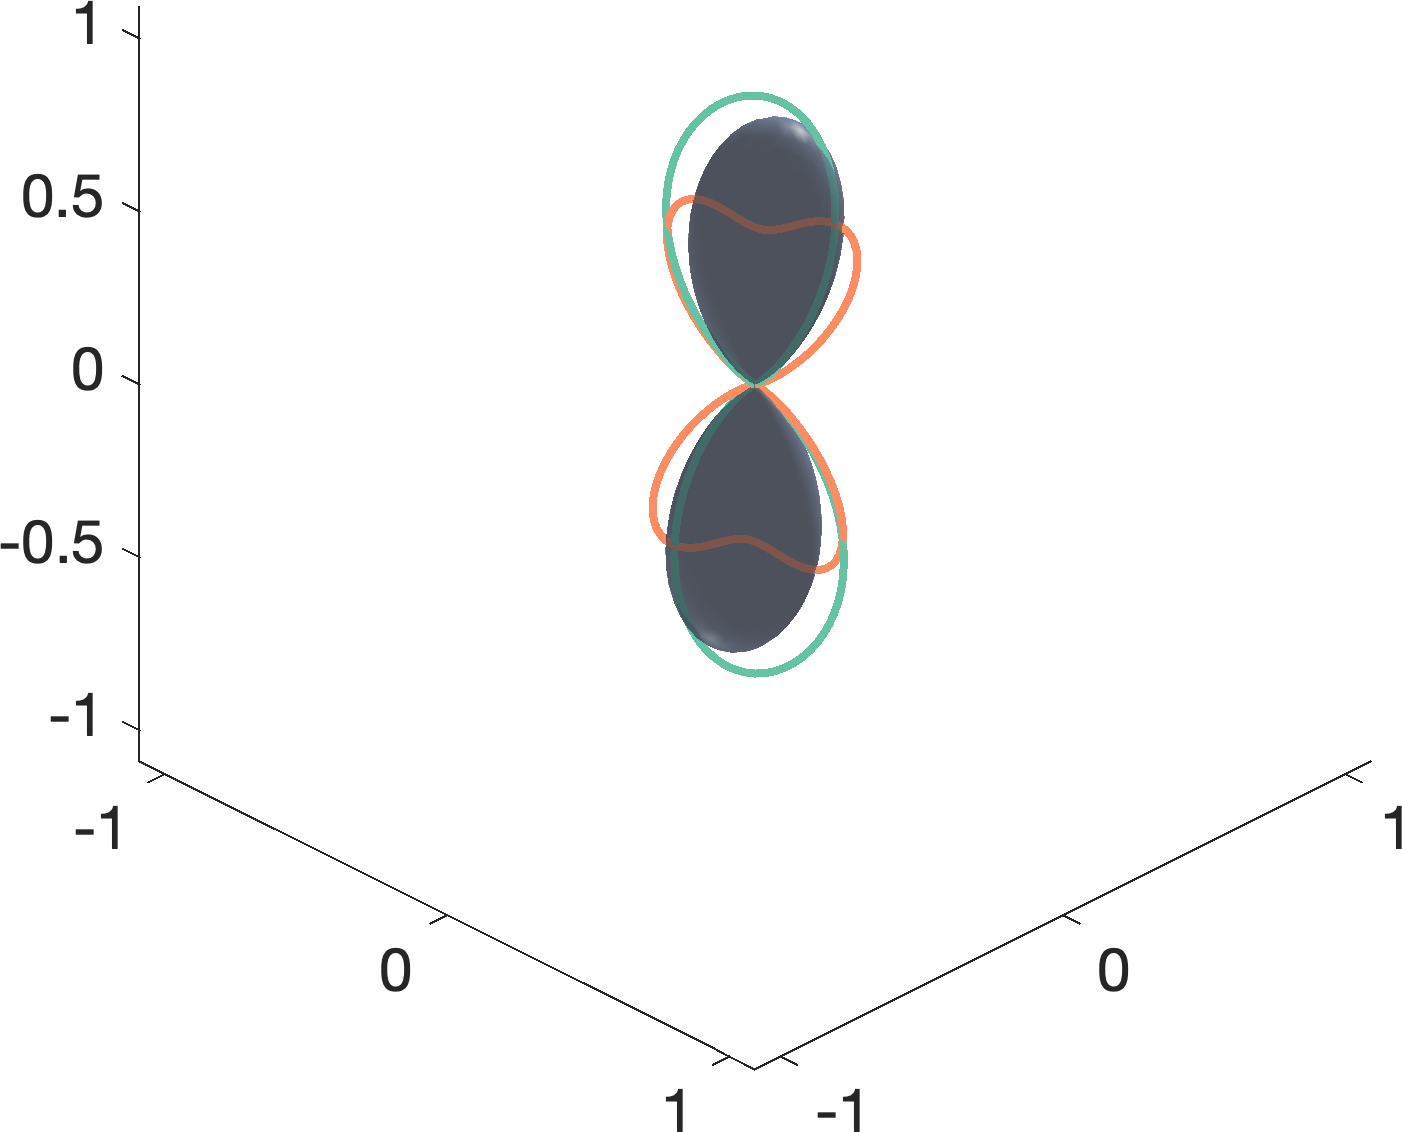
\includegraphics[width=\textwidth]{figures/frf_experiment/EMfibres_fod_3D_b_3000n_3}
    % \caption*{Median}
  \end{subfigure}
  \begin{subfigure}[]{0.245\textwidth}
    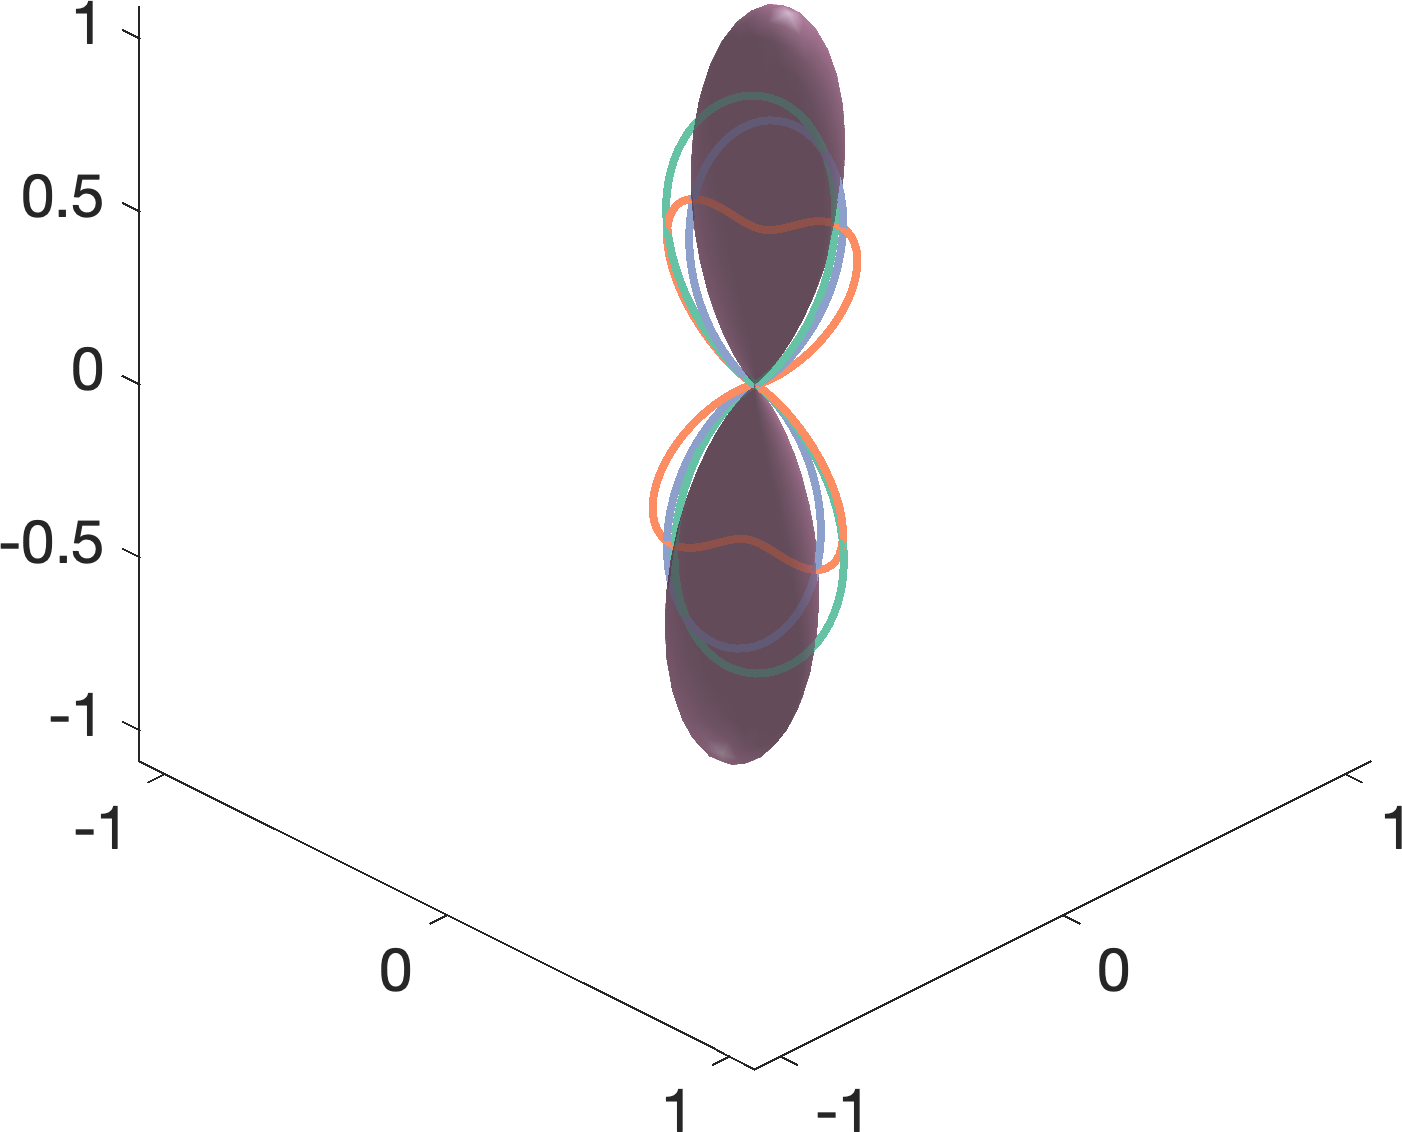
\includegraphics[width=\textwidth]{figures/frf_experiment/EMfibres_fod_3D_b_3000n_4_f1}
    % \caption*{90th percentile}
  \end{subfigure}
j  % \caption{EM fibres}
  % \end{subfigure}
  \end{minipage}
}
  
  \caption[Imapct of the FRF variability on FOD estimation]{Variations in the \ac{FOD} estimated using the 10th percentile, median and 90th percentile signal for the \ac{FRF} for a range of phantoms. Left-to-right: the gold standard \ac{FOD} from microstructure, \ac{FOD} using 10th percentile, \ac{FOD} using median, \ac{FOD} using 90th percentile. 3D glyphs represent the \ac{FOD} for each column and lines show previous \acp{FOD} overlaid. }
  \label{fig:frf_fod_kappa_b2000}
\end{figure}


\begin{figure}
  \centering
  \makebox[\textwidth][c]{
  \begin{minipage}[c]{0.15\textwidth}
    \subcaption{$\kappa = 100$}
  \end{minipage}
  \hfill
  \begin{minipage}[c]{1\textwidth}
  % \begin{subfigure}[]{1\textwidth}
  \begin{subfigure}[]{0.245\textwidth}
    \caption*{Gold standard FOD}
    \includegraphics[width=\textwidth]{figures/frf_experiment/fibres_fod_3D_kappa100_b_3000n_1_snr30}
  \end{subfigure}
  \begin{subfigure}[]{0.245\textwidth}
    \caption*{10th percentile}
    \includegraphics[width=\textwidth]{figures/frf_experiment/fibres_fod_3D_kappa100_b_3000n_2_snr30}
  \end{subfigure}
  \begin{subfigure}[]{0.245\textwidth}
    \caption*{Median}
    \includegraphics[width=\textwidth]{figures/frf_experiment/fibres_fod_3D_kappa100_b_3000n_3_snr30}
  \end{subfigure}
  \begin{subfigure}[]{0.245\textwidth}
    \caption*{90th percentile}
    \includegraphics[width=\textwidth]{figures/frf_experiment/fibres_fod_3D_kappa100_b_3000n_4_snr30}
  \end{subfigure}
  % \caption{$\kappa = 100$}
  % \end{subfigure}
  \end{minipage}
}

 % \begin{subfigure}[]{\textwidth}
\makebox[\textwidth][c]{
  \begin{minipage}[c]{0.15\textwidth}
    \subcaption{$\kappa = 6$}
  \end{minipage}
  \hfill
  \begin{minipage}[c]{\textwidth}
    \begin{subfigure}[]{0.245\textwidth}
    \includegraphics[width=\textwidth]{figures/frf_experiment/fibres_fod_3D_kappa6_b_3000n_1_snr30}
  \end{subfigure}
  \begin{subfigure}[]{0.245\textwidth}
    \includegraphics[width=\textwidth]{figures/frf_experiment/fibres_fod_3D_kappa6_b_3000n_2_snr30}
  \end{subfigure}
  \begin{subfigure}[]{0.245\textwidth}
    \includegraphics[width=\textwidth]{figures/frf_experiment/fibres_fod_3D_kappa6_b_3000n_3_snr30}
  \end{subfigure}
  \begin{subfigure}[]{0.245\textwidth}
    \includegraphics[width=\textwidth]{figures/frf_experiment/fibres_fod_3D_kappa6_b_3000n_4_snr30}
  \end{subfigure}
  % \caption{$\kappa = 6$}
  % \end{subfigure}
  \end{minipage}
}
\makebox[\textwidth][c]{
  \begin{minipage}[c]{0.15\textwidth}
    \subcaption{$\kappa = 2$}
  \end{minipage}
  \hfill
  % \begin{subfigure}[]{\textwidth}
  \begin{minipage}[c]{\textwidth}
    \begin{subfigure}[]{0.245\textwidth}
    \includegraphics[width=\textwidth]{figures/frf_experiment/fibres_fod_3D_kappa2_b_3000n_1_snr30}
  \end{subfigure}
  \begin{subfigure}[]{0.245\textwidth}
    \includegraphics[width=\textwidth]{figures/frf_experiment/fibres_fod_3D_kappa2_b_3000n_2_snr30}
  \end{subfigure}
  \begin{subfigure}[]{0.245\textwidth}
    \includegraphics[width=\textwidth]{figures/frf_experiment/fibres_fod_3D_kappa2_b_3000n_3_snr30}
  \end{subfigure}
  \begin{subfigure}[]{0.245\textwidth}
    \includegraphics[width=\textwidth]{figures/frf_experiment/fibres_fod_3D_kappa2_b_3000n_4_snr30}
  \end{subfigure}
  % \caption{$\kappa = 2$}
  % \end{subfigure}
  \end{minipage}
}
\makebox[\textwidth][c]{
  \begin{minipage}[c]{0.15\textwidth}
    \subcaption{Two crossing}
  \end{minipage}
  \hfill
  \begin{minipage}[c]{\textwidth}
  % \begin{subfigure}[]{\textwidth}
    \begin{subfigure}[]{0.245\textwidth}
    \includegraphics[width=\textwidth]{figures/frf_experiment/twoperp_fod_3D_b_3000n_1_snr30}
  \end{subfigure}
  \begin{subfigure}[]{0.245\textwidth}
    \includegraphics[width=\textwidth]{figures/frf_experiment/twoperp_fod_3D_b_3000n_2_snr30}
  \end{subfigure}
  \begin{subfigure}[]{0.245\textwidth}
    \includegraphics[width=\textwidth]{figures/frf_experiment/twoperp_fod_3D_b_3000n_3_snr30}
  \end{subfigure}
  \begin{subfigure}[]{0.245\textwidth}
    \includegraphics[width=\textwidth]{figures/frf_experiment/twoperp_fod_3D_b_3000n_4_snr30}
  \end{subfigure}
  % \caption{Two crossing}
  % \end{subfigure}
  \end{minipage}
}
\makebox[\textwidth][c]{
  \begin{minipage}[c]{0.15\textwidth}
    \subcaption{Three crossing}
  \end{minipage}
  \hfill
  \begin{minipage}[c]{\textwidth}
  % \begin{subfigure}[]{\textwidth}
    \begin{subfigure}[]{0.245\textwidth}
      \includegraphics[width=\textwidth]{figures/frf_experiment/threeperp_fod_3D_b_3000n_1_snr30}
  \end{subfigure}
  \begin{subfigure}[]{0.245\textwidth}
    \includegraphics[width=\textwidth]{figures/frf_experiment/threeperp_fod_3D_b_3000n_2_snr30}
  \end{subfigure}
  \begin{subfigure}[]{0.245\textwidth}
    \includegraphics[width=\textwidth]{figures/frf_experiment/threeperp_fod_3D_b_3000n_3_snr30}
  \end{subfigure}
  \begin{subfigure}[]{0.245\textwidth}
    \includegraphics[width=\textwidth]{figures/frf_experiment/threeperp_fod_3D_b_3000n_4_snr30}
  \end{subfigure}
  % \caption{Three crossing}
  % \end{subfigure}
  \end{minipage}
}
\makebox[\textwidth][c]{
  \begin{minipage}[c]{0.15\textwidth}
    \subcaption{EM fibres}
  \end{minipage}
  \hfill
  \begin{minipage}[c]{\textwidth}
 % \begin{subfigure}[]{\textwidth}
    \begin{subfigure}[]{0.245\textwidth}
      \includegraphics[width=\textwidth]{figures/frf_experiment/EMfibres_fod_3D_b_3000n_1_snr30}

  \end{subfigure}
  \begin{subfigure}[]{0.245\textwidth}
    \includegraphics[width=\textwidth]{figures/frf_experiment/EMfibres_fod_3D_b_3000n_2_snr30}
    % \caption*{10th percentile}
  \end{subfigure}
  \begin{subfigure}[]{0.245\textwidth}
    \includegraphics[width=\textwidth]{figures/frf_experiment/EMfibres_fod_3D_b_3000n_3_snr30}
    % \caption*{Median}
  \end{subfigure}
  \begin{subfigure}[]{0.245\textwidth}
    \includegraphics[width=\textwidth]{figures/frf_experiment/EMfibres_fod_3D_b_3000n_4_snr30}
    % \caption*{90th percentile}
  \end{subfigure}
  % \caption{EM fibres}
  % \end{subfigure}
  \end{minipage}
}
\end{figure}




\begin{figure}
  \centering
  \begin{subfigure}[]{\textwidth}
  \begin{subfigure}[]{0.32\textwidth}
    \includegraphics[width=\textwidth]{figures/frf_experiment/fibres_fod_3D_kappa2_b_1000n_4}
  \end{subfigure}
  ~
  \begin{subfigure}[]{0.32\textwidth}
    \includegraphics[width=\textwidth]{figures/frf_experiment/fibres_fod_3D_kappa2_b_2000n_4}
  \end{subfigure}
  ~
  \begin{subfigure}[]{0.32\textwidth}
    \includegraphics[width=\textwidth]{figures/frf_experiment/fibres_fod_3D_kappa2_b_3000n_4}
  \end{subfigure}
  \caption{$\kappa = 2$}
  \end{subfigure}

  \begin{subfigure}[]{\textwidth}
  \begin{subfigure}[]{0.32\textwidth}
    \includegraphics[width=\textwidth]{figures/frf_experiment/twoperp_fod_3D_b_1000n_4}
  \end{subfigure}
  ~
  \begin{subfigure}[]{0.32\textwidth}
    \includegraphics[width=\textwidth]{figures/frf_experiment/twoperp_fod_3D_b_2000n_4}
  \end{subfigure}
  ~
  \begin{subfigure}[]{0.32\textwidth}
    \includegraphics[width=\textwidth]{figures/frf_experiment/twoperp_fod_3D_b_3000n_4}
  \end{subfigure}
  \caption{Two crossing}
  \end{subfigure}

  \begin{subfigure}[]{\textwidth}
  \begin{subfigure}[]{0.32\textwidth}
    \includegraphics[width=\textwidth]{figures/frf_experiment/threeperp_fod_3D_b_1000n_4}
  \end{subfigure}
  ~
  \begin{subfigure}[]{0.32\textwidth}
    \includegraphics[width=\textwidth]{figures/frf_experiment/threeperp_fod_3D_b_2000n_4}
  \end{subfigure}
  ~
  \begin{subfigure}[]{0.32\textwidth}
    \includegraphics[width=\textwidth]{figures/frf_experiment/threeperp_fod_3D_b_3000n_4}
  \end{subfigure}
  \caption{Three crossing}
  \end{subfigure}
  \begin{subfigure}[]{\textwidth}
  \begin{subfigure}[]{0.32\textwidth}
    \includegraphics[width=\textwidth]{figures/frf_experiment/EMfibres_fod_3D_b_1000n_4}
    \caption*{$b=\SI{1000}{\second\per\milli\metre\squared}$}
  \end{subfigure}
  ~
  \begin{subfigure}[]{0.32\textwidth}
    \includegraphics[width=\textwidth]{figures/frf_experiment/EMfibres_fod_3D_b_2000n_4}
    \caption*{$b=\SI{2000}{\second\per\milli\metre\squared}$}
  \end{subfigure}
  ~
  \begin{subfigure}[]{0.32\textwidth}
    \includegraphics[width=\textwidth]{figures/frf_experiment/EMfibres_fod_3D_b_3000n_4}
    \caption*{$b=\SI{3000}{\second\per\milli\metre\squared}$}
  \end{subfigure}
  \caption{EM fibres}
  \end{subfigure}
  \caption[Variation in \acs{FOD} estimated at $b = 1000,2000,\SI{3000}{\second\per\milli\metre\squared}$]{Variation in \ac{FOD} estimated using 10th percentile, median and 90th percentile \ac{FRF} at $b = 1000,2000,\SI{3000}{\second\per\milli\metre\squared}$ (left-to-right) for (a) the $\kappa=2$ phantom, (b) the two crossing bundles phantoms  (c) the three crossing bundles phantom and (d) the EM fibres. Green 3D surface is gold standard \ac{FOD} from microstructure and lines outline the \ac{FOD} using the 10th percentile, median and 190th percentile signals. }
  \label{fig:frf_fod_b123}
\end{figure}

The variation in the \ac{FRF} for each fibre leads to a variation in the estimated \ac{FOD} as seen in \Cref{fig:frf_fod_kappa_b2000}.
Again, the magnitude of differences in \ac{FOD} tends to depend on the complexity of the fibre arrangements since the more complex arrangements have more variation in the \ac{FRF}.
The resultant \ac{FOD} is dependent on the $b$-value as demonstrated by \Cref{fig:frf_fod_b123}. While the direction of peaks in the \ac{FOD} does not differ greatly at different $b$-values, the overall shape can change. 
Generally, the \ac{FOD} calculated from \ac{SD} picks out the correct main peak direction that is seen in the gold standard \ac{FOD} from the microstructure, with differences in the overall peak amplitude and shape.
A notable exception to this is the $\kappa=2$ phantom which at low $b$-value identifies two peaks with some \acp{FRF} which are not present in the gold standard \ac{FOD}.

\subsection{Extracellular contribution}
\label{sec:frf_res_extracellular}


\begin{figure}
  \centering
  \begin{subfigure}[]{0.4\textwidth}
    \includegraphics[width=\textwidth]{figures/frf_experiment/in_ex_tot_Kappa_2.png}
    \caption{}
  \end{subfigure}
  ~
  \begin{subfigure}[]{0.4\textwidth}
    \includegraphics[width=\textwidth]{figures/frf_experiment/in_ex_tot_Kappa_6.png}
    \caption{}
  \end{subfigure}

  \begin{subfigure}[]{0.4\textwidth}
    \includegraphics[width=\textwidth]{figures/frf_experiment/in_ex_tot_Kappa_100}
    \caption{}
  \end{subfigure}
  ~
  \begin{subfigure}[]{0.4\textwidth}
    \includegraphics[width=\textwidth]{figures/frf_experiment/in_ex_tot_Gamma_Cylinders}
    \caption{}
  \end{subfigure}

  \caption[Intra, extra and overall signal as a function of b-value]{Intra, extra and overall radial signal as a function of b-value for (a) $\kappa=2$, (b) $\kappa=6$, (c) $\kappa=100$, (d) Cylinders.}
  \label{fig:frf_intra_ex_rad}
\end{figure}

\begin{figure}
  \centering
  \includegraphics[width=0.85\textwidth]{figures/frf_experiment/sig_sh_b2000}
  \caption[Extracellular signal fraction as a function of b-value]{Total, intracellular and extracellular signal for $b = \SI{2000}{\second\per\milli\metre\squared}$ for a $\kappa = 2, 6$ and $100$ and straight parallel cylinders. }
  \label{fig:frf_extra_sh}
\end{figure}

\begin{figure}
  \centering
  \begin{subfigure}[]{0.4\textwidth}
    \includegraphics[width=\textwidth]{figures/frf_experiment/fod_inex_b3000_kappa2}
    \caption{}
  \end{subfigure}
  ~
  \begin{subfigure}[]{0.4\textwidth}
    \includegraphics[width=\textwidth]{figures/frf_experiment/fod_inex_b3000_kappa6}
    \caption{}
  \end{subfigure}

  \begin{subfigure}[]{0.4\textwidth}
    \includegraphics[width=\textwidth]{figures/frf_experiment/fod_inex_b3000_kappa100}
    \caption{}
  \end{subfigure}
  ~
  \begin{subfigure}[]{0.4\textwidth}
    \includegraphics[width=\textwidth]{figures/frf_experiment/fod_inex_b3000_GamCyl}
    \caption{}
  \end{subfigure}

  \caption[Impact of the extracellular space on FOD estimate]{Impact of the extracellular space on FOD estimation for (a) $\kappa=2$, (b) $\kappa=6$, (c) $\kappa=100$, (d) Cylinders. When using the `ideal' \ac{FRF} from the intracellular signal, the \ac{FOD} estimated varies quite significantly compared to when using the `practical' \ac{FRF} using the total signal.}
  \label{fig:frf_intra_ex_fod}
\end{figure}

The radial \ac{dMRI} signal from the extracellular space decays rapidly with b-value when compared to the intracellular space as seen in \Cref{fig:frf_intra_ex_rad}.
In the case of parallel (or close to parallel) fibres in \Cref{fig:frf_intra_ex_rad}c\&d, the intracellular signal is constant with b-value as the fibres act like completely restricting compartments in the radial direction while in the case of dispersion (\Cref{fig:frf_intra_ex_rad}a\&b), the intracellular signal decays, though at a slower rate than the extracellular signal.

The extracellular signal does not entirely decay, even at very high b-values and straight, parallel cylinders, contrary to the findings of Raffelt et al. \cite{Raffelt2012}.

In addition to the non-zero contribution of the extracellular space, the shape of the extracellular signal is different to the intracellular space, particularly in complex fibre arrangements as seen in \Cref{fig:frf_extra_sh}.
In the phantoms with higher orientation dispersion, the extracellular signal is more isotropic while for parallel fibres, the extracellular signal is much closer to the shape of the intracellular signal.

\section{Discussion}
\label{sec:frf_discussion}

\subsection{Per-fibre response function}
\label{sec:frf_discussion_perfibre}
The microscopic variations in fibre morphology challenge the assumption in \acl{SD} techniques that there exists a unique and shared \acl{FRF} even within a single voxel.
Here we used \ac{dMRI} simulations to demonstrate that variations in individual axonal morphology do indeed lead to different response functions per-fibre which in turn can have a knock-on effect on \ac{SD} techniques to estimate the \acl{FOD}.

As demonstrated in \Cref{fig:frf_prctiles_kappa_b2000,fig:frf_prctiles_b123}, the response function can vary quite a lot across different fibres, particularly in complex fibre arrangements such as the three crossing bundles scenario (\Cref{fig:frf_prctiles_kappa_b2000}e).
Indeed, the variation in responses in fibres reconstructed from real \ac{EM} images of \acl{WM} is large, similar to that of the ConFiG three crossing simulations, and much larger than \ac{ConFiG} phantoms containing a single fibre bundle.
This suggests that there is in fact more variation in real axons than in the axons generated by \ac{ConFiG}, even in simple arrangements of a single bundle of fibres. This is something that may be used to inform future versions of \ac{ConFiG} to generate more realistic phantoms.

In the main, the largest variation in the per-fibre response, as well as the largest difference between cylinders and realistic axons happens in the axial direction which is to be expected. Even with diameter variations and undulation, the radial diffusion is still strongly restricted under the assumption of no axonal permeability, while recent studies have shown that real axonal morphology causes time-dependent deviations from Gaussian diffusivity along the axial direction \cite{Lee2019a}.

Variations in the \ac{FRF} have an impact on the estimated \ac{FOD} as demonstrated in \Cref{fig:frf_fod_kappa_b2000,fig:frf_fod_b123}. In the simplest fibre arrangements with the lowest dispersion (\Cref{fig:frf_fod_kappa_b2000}a\&b), the \ac{FRF} variation is relatively small and so the \ac{FOD} variation is small and the \ac{FOD} peak directions match the gold standard \ac{FOD} well, however in the $\kappa=2$ case, the \ac{FOD} varies greatly when using different \ac{FRF}s (\Cref{fig:frf_fod_kappa_b2000}c and \Cref{fig:frf_prctiles_b123}a).

Interestingly, when using the 10th percentile and median \ac{FRF}, the \ac{FOD} seems to pick out two crossing bundles which are not present in the gold standard \ac{FOD}, while the 90th percentile \ac{FRF} picks up one dispersed bundle much closer to the gold standard \ac{FOD}. On top of this, the relative amplitudes of the \ac{FOD} change with $b$-value as seen in \Cref{fig:frf_prctiles_b123}a in which the median and the 10th percentile \ac{FOD} changes from two distinct peaks at $b=\SI{1000}{\second\per\milli\metre\squared}$ to one wider merged peak at $b=\SI{3000}{\second\per\milli\metre\squared}$.
These kinds of effects could have significant impacts on tractography techniques which use the \ac{FOD} to trace fibre bundles through the brain.

In the case of crossing fibres, the \ac{FOD} varies depending on the \ac{FRF} used too. In the case of two crossing bundles of fibres (\Cref{fig:frf_fod_kappa_b2000}d), each bundle responds in a similar way, with peak directions and amplitudes largely unaffected by the \ac{FRF} used and matching the gold standard \ac{FOD} well.
In the three perpendicular bundle case, however, peak amplitudes are affected by the \ac{FRF} used as seen in \Cref{fig:frf_fod_kappa_b2000}e and \Cref{fig:frf_prctiles_b123}c, in which different \acp{FRF} create \acp{FOD} with different relative peak amplitudes. The 90th percentile \ac{FRF} selects the largest peak very strongly, creating smaller perpendicular peaks while the 10th percentile (and, in fact gold standard) \ac{FRF} pick out more even lobes.
This is significant because as shown by Schilling et al.\cite{Schilling2019}, even changes in \ac{FOD} peak amplitudes without peak direction changes can have an impact on tractography results.
%with the \ac{SD} based \ac{FOD} picking out one large and small peak in \Cref{fig:frf_fod_b123}b with the small peak much smaller than the gold standard \ac{FOD}.This is significant because as shown by Schilling et al.\cite{Schilling2019}, even changes in \ac{FOD} peak amplitudes without peak direction changes can have an impact on tractography results.
%Further, the orientation of the vertical lobes in \Cref{fig:frf_fod_b123} changes from $b=1000$ to $b=\SI{3000}{\second\per\milli\metre\squared}$ which again could have a significant impact on tractography results.

In the real \ac{EM} fibres, the large differences in \ac{FRF} lead to large differences in the \ac{FOD} as seen in \Cref{fig:frf_fod_kappa_b2000}f and \Cref{fig:frf_fod_b123}d. Similarly to the $\kappa=2$ case, the 10th percentile \ac{FRF} seems to pick out two crossing peaks, while the others pick out a single peak, closer to the gold standard \ac{FOD}. This effect is dependent on $b$-value, with the two peaks at $b = \SI{1000}{\second\per\milli\metre\squared}$ merging into one at $b=\SI{3000}{\second\per\milli\metre\squared}$.
One possible explanation for this finding two peaks where there in fact is only one be that the number of fibres in the phantom is lower than you'd expect in a full \ac{dMRI} phantom (typically ~300 fibres per phantom) so the sampling of the orientation distribution may appear to be two peaks. Another possible explanation is that the Tikhonov regularisation in \ac{CSD} \cite{Tournier2007} encourages directions in which there is little diffusion to zero and it may be over-regularising in the $\kappa=2$ and \ac{EM} fibres cases.
%As above, even though the \ac{FOD} is relatively simple and varies only in amplitude, this could have an impact on tractography results.


Additionally, these simulations lend further support to challenge the assumption that \ac{FRF} is constant across the brain as differences in the median \ac{FRF} per phantom demonstrate that the overall \ac{FRF} from different fibre arrangements will be different as a result of the different axonal morphology in each environment. Further, as demonstrated by the \ac{FOD} experiments, small changes in the \ac{FRF} can lead to significant changes in the estimated \ac{FOD}, meaning that using the wrong \ac{FRF} in different brain regions could have large impacts on \ac{FOD} based techniques such as tractography. 


\subsection{Extracellular contribution}
\label{sec:frf_discussion_extra_contribution}
As seen in \Cref{fig:frf_intra_ex_rad,fig:frf_extra_sh}, the contribution of the extracellular space to the overall signal is small but non-zero.
The radial extracellular signal decays more quickly than the intracellular signal, even in highly dispersed fibres, but does not completely decay even at relatively high $b$-values (around $15\%$ extracellular signal fraction at \SI{3000}{\second\per\milli\metre\squared} and $10\%$ at \SI{5000}{\second\per\milli\metre\squared}).
This brings into question the assumption inherent in some \ac{SD} techniques such as \ac{AFD} that the extracellular space is negligible and is also contrary to the simulation experiment performed by Raffelt et al. \cite{Raffelt2012} who show the extracellular signal decaying to negligible levels by $b=\SI{3000}{\second\per\milli\metre\squared}$. The exact cause of this difference requires further investigation, especially for the cylinder phantom which should be comparable.

The signals from the intracellular and extracellular space also do not always have the same shape, with highly dispersed fibres showing a more isotropic signal in the extracellular space than the intracellular space (\Cref{fig:frf_extra_sh}).
This again can question the assumption that the impact of the extracellular space is negligible on \ac{SD} techniques, particularly as the shape of the extracellular signal varies in different fibre arrangements. This may lead to \ac{FRF}s estimated in one environment misestimating the \ac{FOD} in an environment with a different underlying geometry.

\begin{comment}
As an example of this, \Cref{fig:frf_different_FRF} shows the \ac{FOD} estimated using the \ac{FRF} from the total signal from both the $\kappa=100$ and $\kappa=2$ phantoms on the signal from the $\kappa=2$ phantom. 
\begin{figure}
  \centering
  \includegraphics[width=0.6\textwidth]{figures/frf_experiment/fod_b3000_frf_kappa100_sig_kappa2}
  \caption[FOD using FRF from $\kappa=100$ and signal from $\kappa=2$]{FOD estimated using the FRF from both $\kappa=100$ and $\kappa=2$ signal from $\kappa=2$}
  \label{fig:frf_different_FRF}
\end{figure}
\end{comment}

This contribution of the extracellular space additionally impacts \ac{FOD} estimation with \acl{SD} as shown in \Cref{fig:frf_intra_ex_fod}.
When using the `ideal' \ac{FRF} from the intracellular signal only compared to the `practical' \ac{FRF} from the total signal, the estimated \ac{FOD} varies and although the variation is largely in the \ac{FOD} amplitude, this will have an impact on tractography techniques. Additionally, in the $\kappa=2$ case, the \ac{FOD}s have slightly different primary directions, which will also affect tractography techniques.

\subsection{Limitations and future work }
\label{sec:frf_limitations}
In this work we investigated how complex fibre morphology affects \acl{SD} techniques using a \ac{dMRI} scheme chosen to use clinically feasible gradient strength and duration, though it may be possible that other measurement schemes exhibit greater or lesser sensitivity to these effects. For instance Yeh et al. \cite{Yeh2010} have shown that the gradient pulse duration can impact fibre orientation estimation.
Another factor to investigate is the impact of the diffusion time on the observed effects, since longer diffusion times can `smooth out' these microscopic morphological variations as spins are able to diffuse further.

The simulations presented here are performed with no noise added, representing an ideal case of infinite \ac{SNR}. In reality, \ac{dMRI} measurements would be expected to have an \ac{SNR} between 15 and 100. The impact of noise on the effects presented here will be the subject of future work to investigate whether realistic noise levels may mask these differences.

Throughout this work we have referred to the \ac{FOD} generated from the phantom microstructure as the gold standard \ac{FOD} in inverted commas. This is deliberate since, as mentioned in \Cref{sec:frf_true_frf_extraction,sec:micro_limitations}, the definition of the \ac{FOD} from microstructure does not entirely correspond to that from \ac{dMRI}.
Efforts have been made to make the two \acp{FOD} comparable in this work by defining the gold standard \ac{FOD} using a single direction per fibre and normalising all \acp{FOD} to one, however future work will investigate the best way to represent these \acp{FOD}.

The variability that is demonstrated in the per-fibre response in this experiment is suggested to arise due to the complexity of fibre morphology introduced due to complex fibre arrangements.
This seems to be case, as shown in \Cref{fig:frf_prctiles_kappa_b2000}, though the exact nature of the link is not known for certain since there are many sources of morphological complexity (undulation, beading, non-circular cross-sections, etc.) which could all contribute to these variations.
Future work will aim to isolate each of these effects to probe which morphological features have the largest impact on the \ac{FRF}/\ac{FOD}. Should these effects be understood, it may be possible to estimate them from the \ac{dMRI} signal to improve the accuracy of \ac{SD} techniques.

Another important consideration is that in this work we use \acl{CSD} as in MRtrix3 \cite{Tournier2019}, however there are wide range of \ac{SD} techniques for \ac{FOD} estimation, each with slightly different derivations and assumptions.
While this will affect the \acp{FOD} presented in this work, though the per-fibre signals and compartmental signals presented in \Cref{fig:frf_prctiles_kappa_b2000,fig:frf_extra_sh} do not rely on any \ac{SD} model, so the \ac{FRF} variations will impact any models which use the \ac{FRF}.

It is worth pointing out that here we merely demonstrate that the response varies on a per-fibre basis, meaning that the concept of a fibre response function needs to be treated carefully. Most \ac{SD} techniques estimate their \ac{FRF} from averaging across a number of voxels, meaning that the \ac{FRF} is an average single bundle response (including many fibres, extracellular space, other cells etc.) rather than purely a \emph{fibre} response function.
The variability in the per-fibre response may contribute less to the variable overall \ac{FRF} seen across the brain in previous studies \cite{Schilling2019,Christiaens2020} than other factors such as the extracellular space but it should be considered. 

It is also worth noting that this effect will impact other \ac{dMRI} modelling techniques which model the signal as a combination of a diffusion response with an orientation distribution. For instance, \ac{NODDI} \cite{Zhang2012} models the intracellular signal with a Watson distribution as the orientation component and diffusion in sticks as the MR response, assuming that all the fibres can be treated as sticks.
As shown here, microscopic variations in fibre morphology mean that the signals from each fibre are not identical and this could affect results of \ac{NODDI} and other similar models.
Future work will aim to investigate this effect and investigate whether it is possible for it to be accounted for.

\section{Conclusion}
\label{sec:frf_conclusion}
The complex axonal morphology introduced by axons packing together in complex arrangements leads to differences in the \ac{dMRI} response across different fibres.
These variations in per-fibre response functions lead to differences in the \ac{FOD} estimated using \acl{CSD}, suggesting that the assumption of a single \ac{FRF} across all fibres and all voxels may need to be considered carefully.
Further, the extracellular space contributes to the overall signal, even at high b-values ($>$\SI{3000}{\second\per\milli\metre\squared}) obscuring the `ideal' \ac{FRF} from the intracellular space which leads to a `practical' \ac{FRF} which leads to differences in the \ac{FOD}.

All of this means that the interpretation of the \ac{FRF} and \ac{FOD} in \acl{SD} needs to be carefully considered and future models may seek to disentangle some of these effects for more accurate \ac{FRF} and \ac{FOD} estimation. 


%%% Local Variables:
%%% mode: latex
%%% TeX-master: "../main"
%%% End:
